\subsection{High and low mBB control region}
\label{app:boosted_mbbcontrolregion_highlow}

Figure~\ref{fig:boosted_mbbcrHighLow_mainplots}, \ref{fig:boosted_mbbcrHighLow_largerjet}, \ref{fig:boosted_mbbcrHighLow_wwsystem},
\ref{fig:boosted_mbbcrHighLow_whad}, \ref{fig:boosted_mbbcrHighLow_wlep}, \ref{fig:boosted_mbbcrHighLow_lepton}, \ref{fig:boosted_mbbcrHighLow_whad_leadjet}
and \ref{fig:boosted_mbbcrHighLow_whad_subleadjets} shows the kinematic distribution of events 
in the high ($m_\text{Large-R jet} > 140~\GeV $) and low ($m_\text{Large-R jet} < 90~\GeV $) mBB control region.

\begin{figure}[!h]
\begin{center}
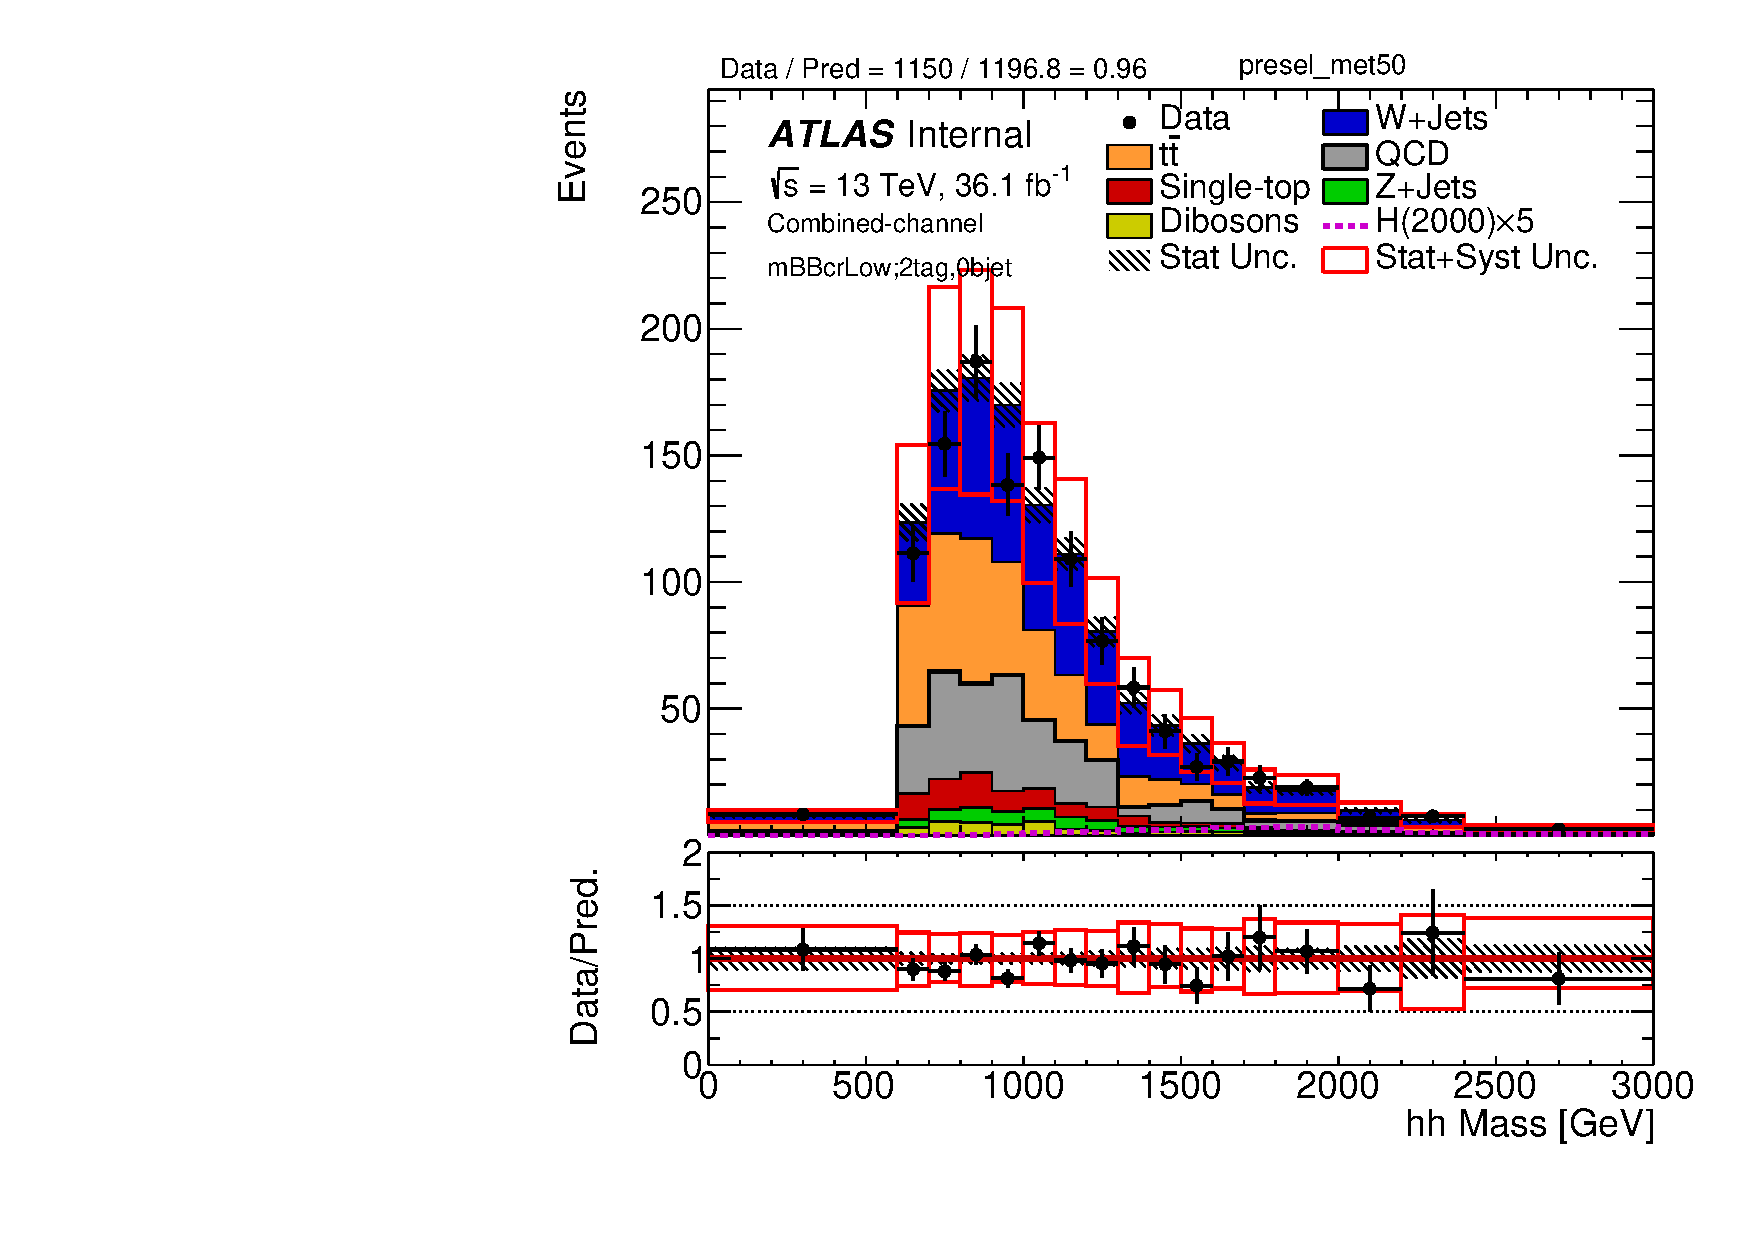
\includegraphics[scale=0.33]{./figures/boosted/PlotByMbbRegions/DataMC_2tag_0bjet_mbbcrLow_lepton_presel_met50_hhMassRebin1}                                                                        
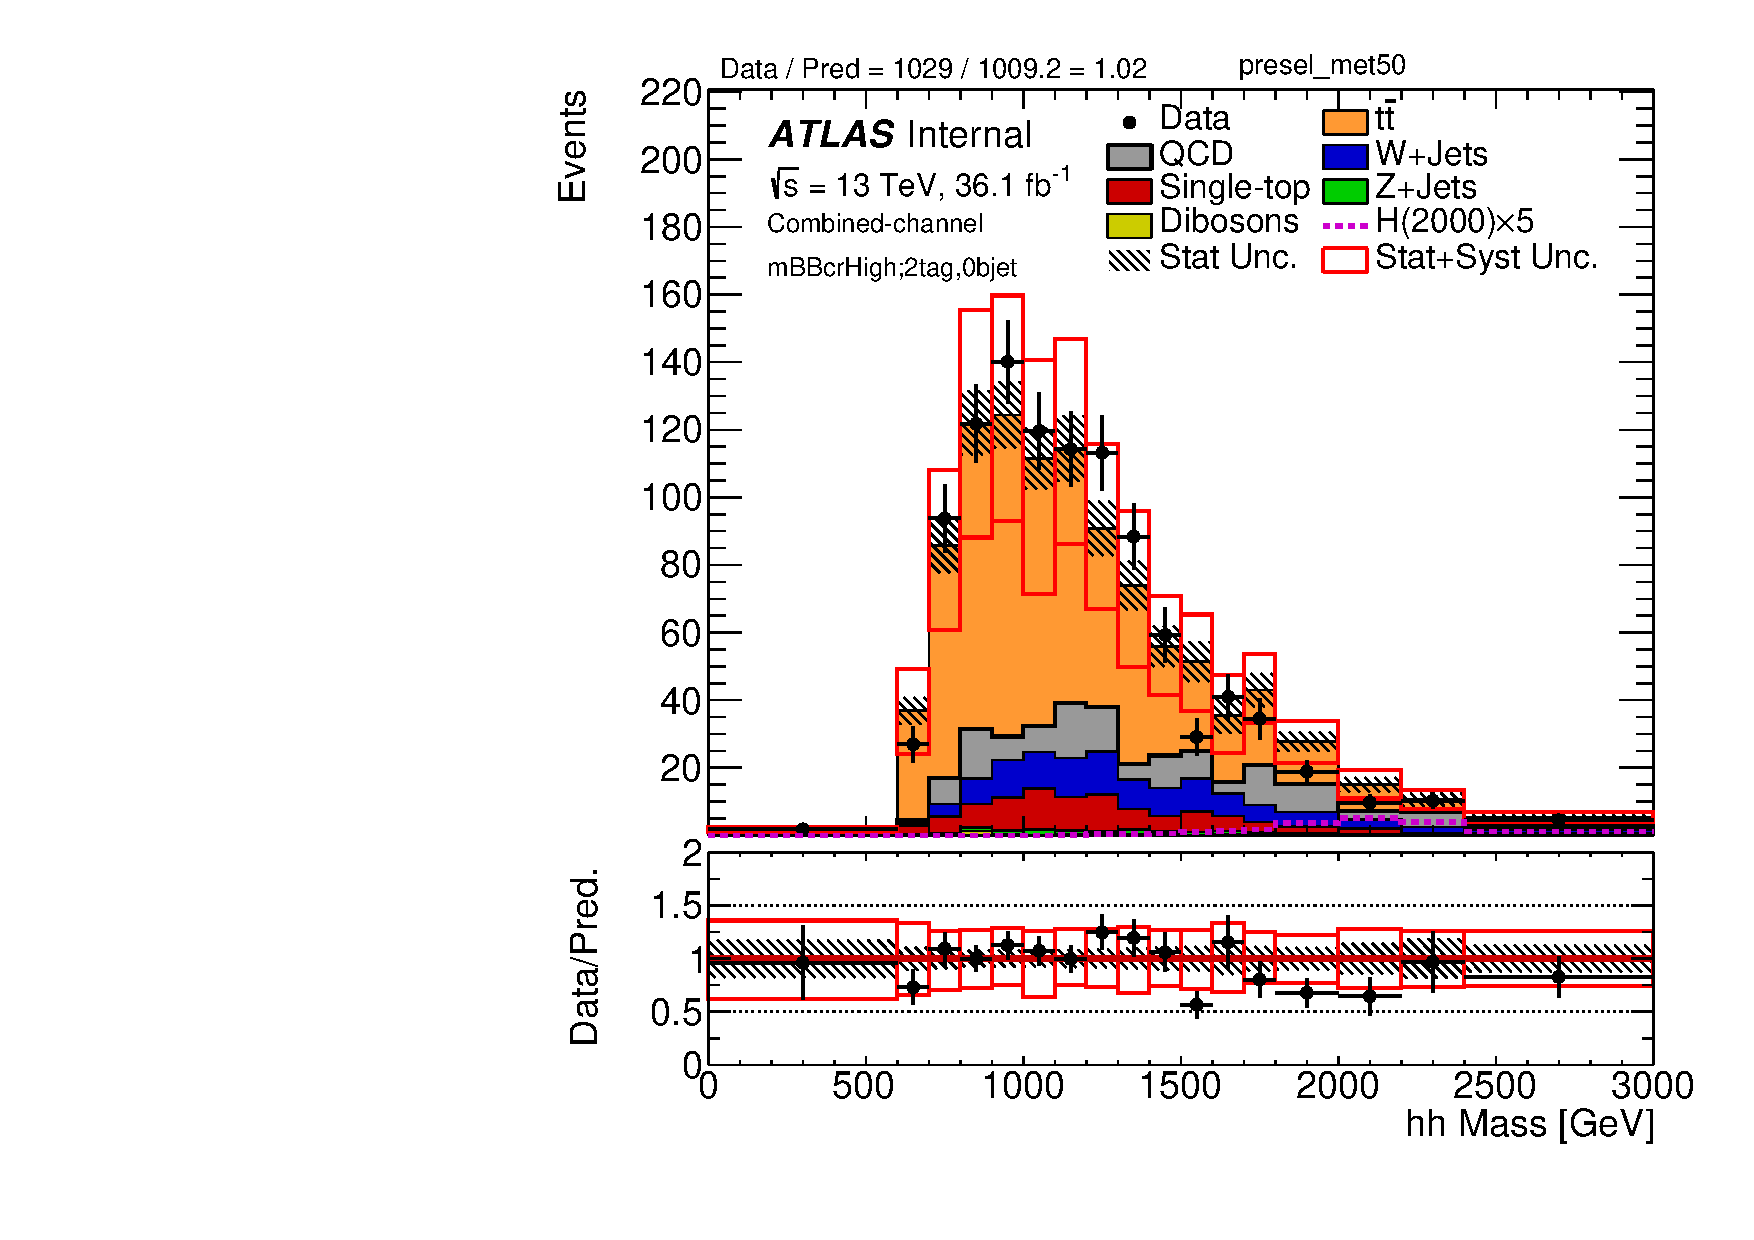
\includegraphics[scale=0.33]{./figures/boosted/PlotByMbbRegions/DataMC_2tag_0bjet_mbbcrHigh_lepton_presel_met50_hhMassRebin1}                                                                       
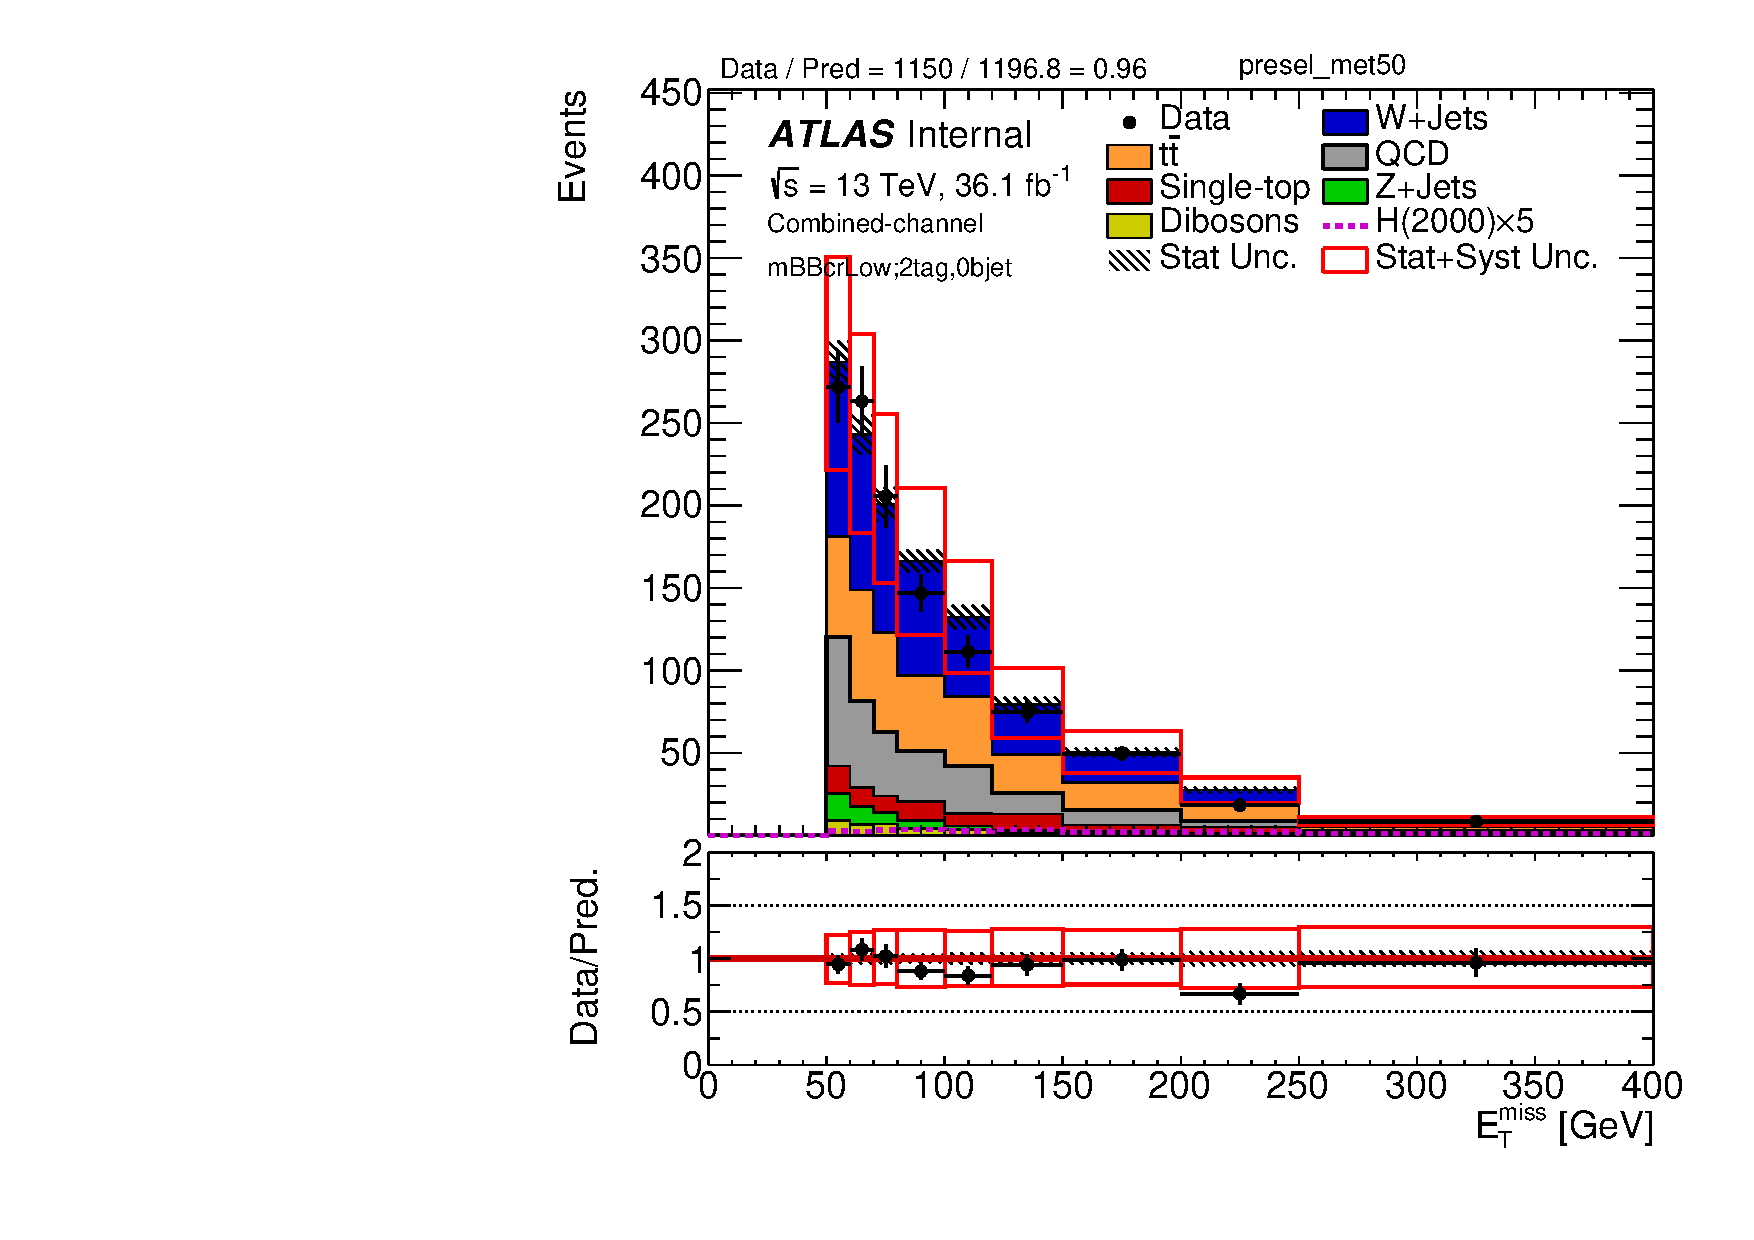
\includegraphics[scale=0.33]{./figures/boosted/PlotByMbbRegions/DataMC_2tag_0bjet_mbbcrLow_lepton_presel_met50_MET}                                                                                 
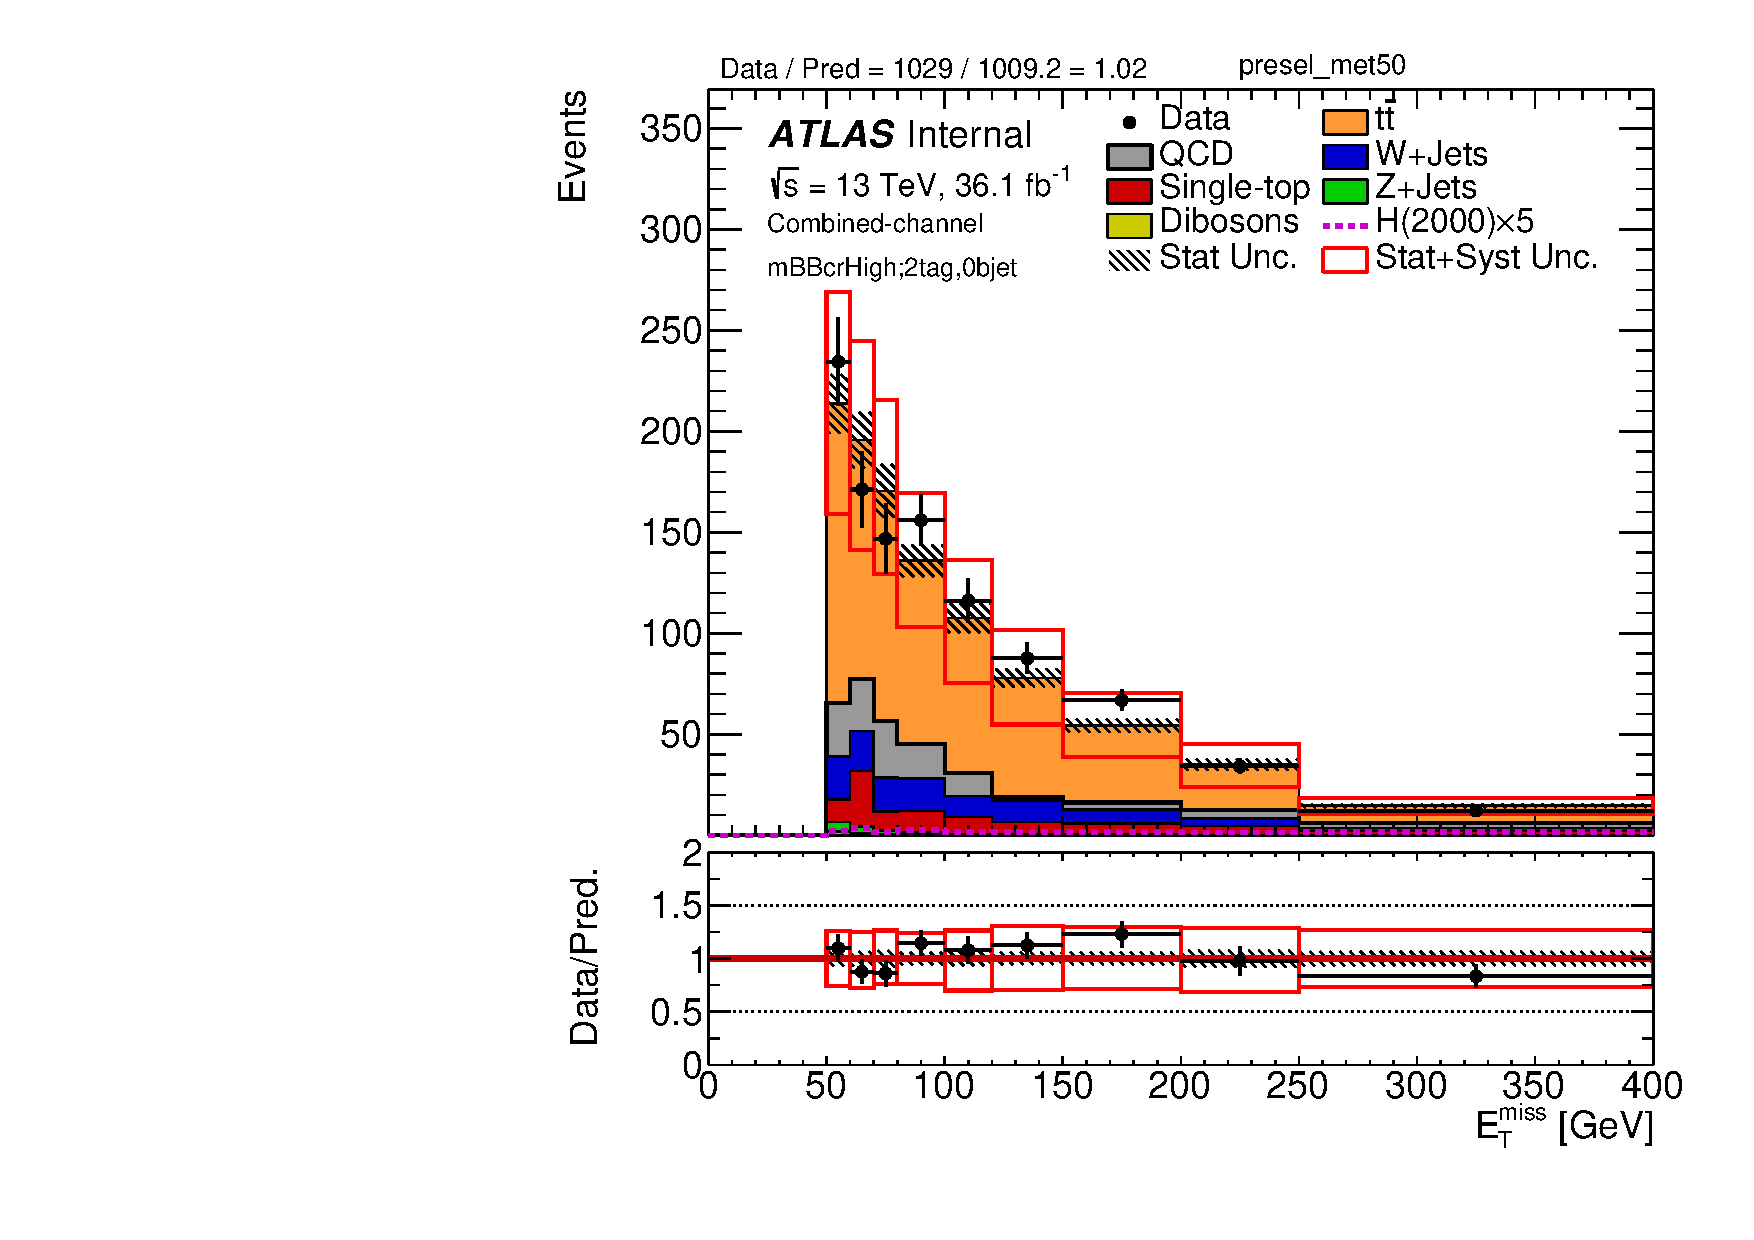
\includegraphics[scale=0.33]{./figures/boosted/PlotByMbbRegions/DataMC_2tag_0bjet_mbbcrHigh_lepton_presel_met50_MET}                                                                                
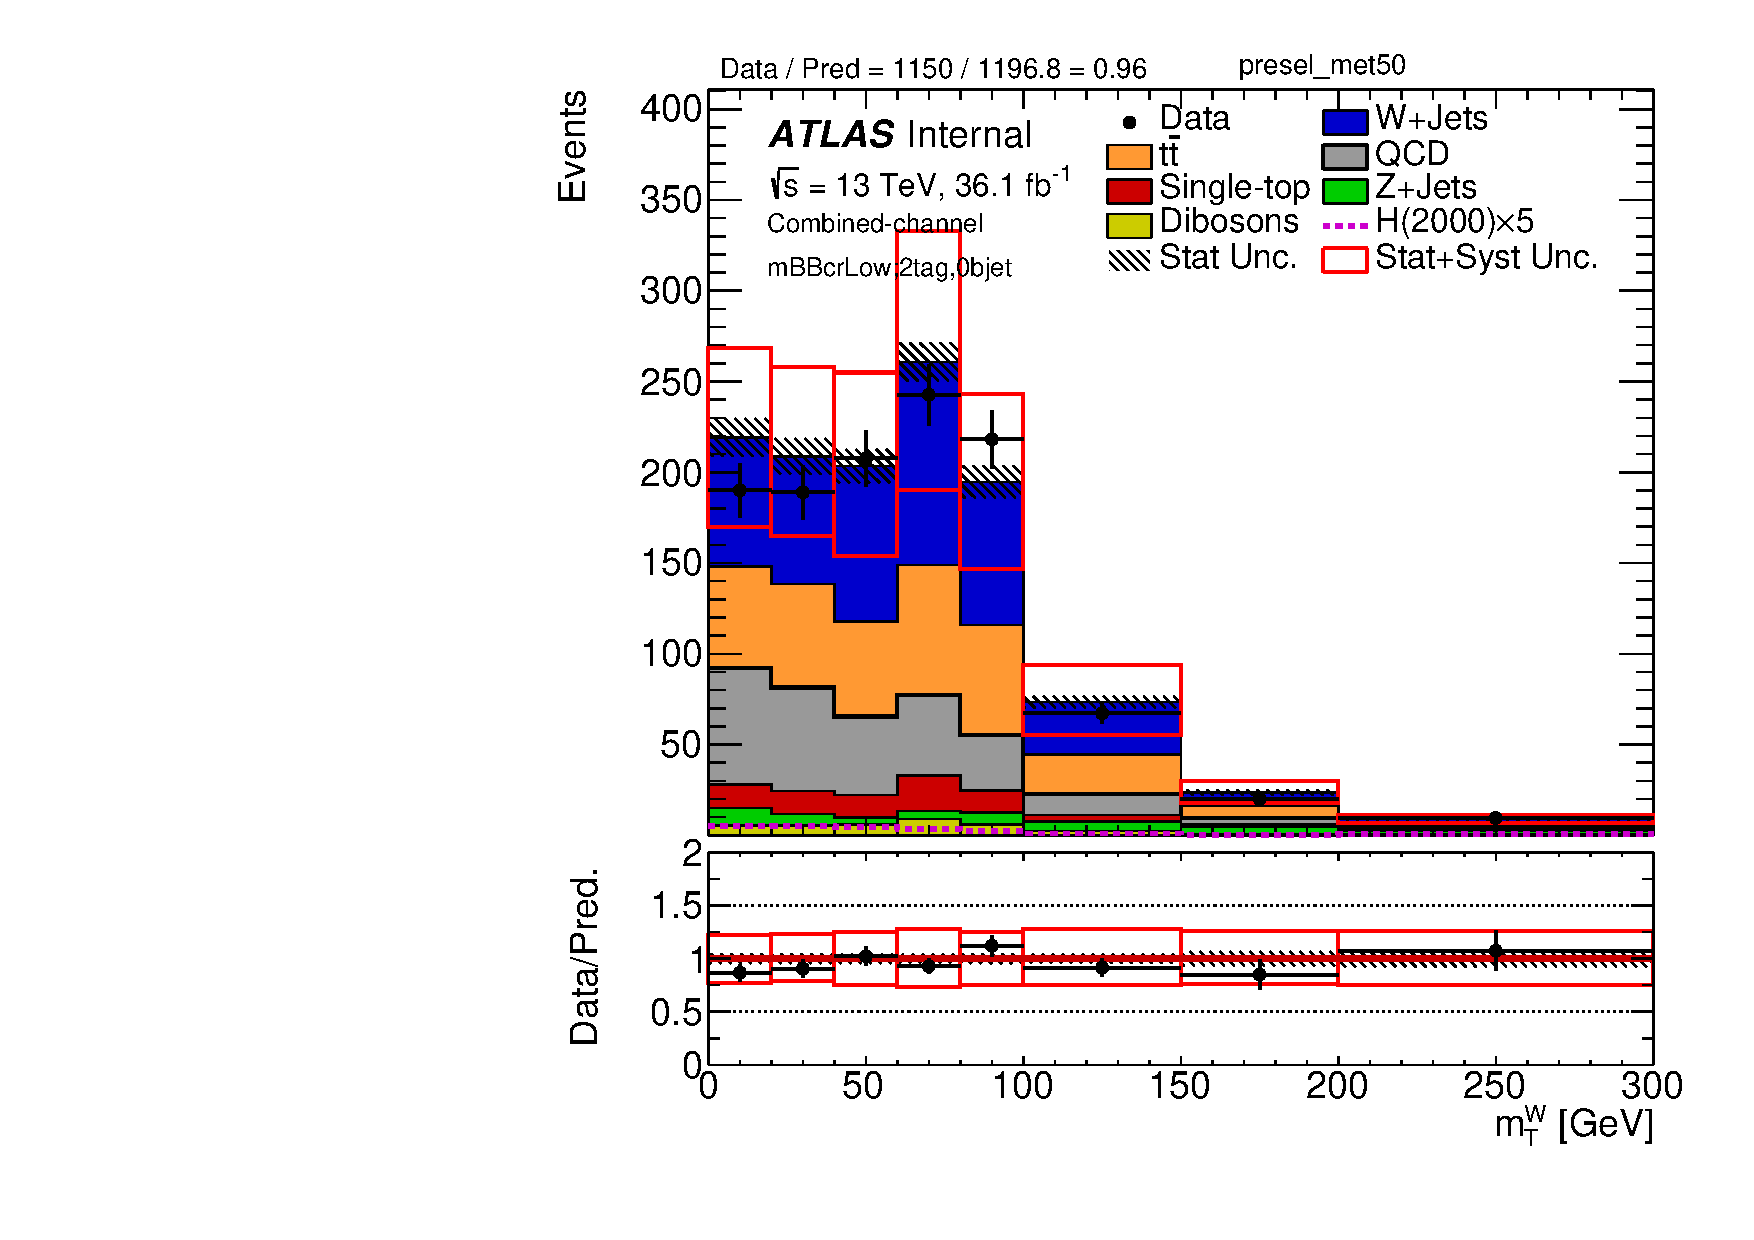
\includegraphics[scale=0.33]{./figures/boosted/PlotByMbbRegions/DataMC_2tag_0bjet_mbbcrLow_lepton_presel_met50_WlepMtATLAS}                                                                         
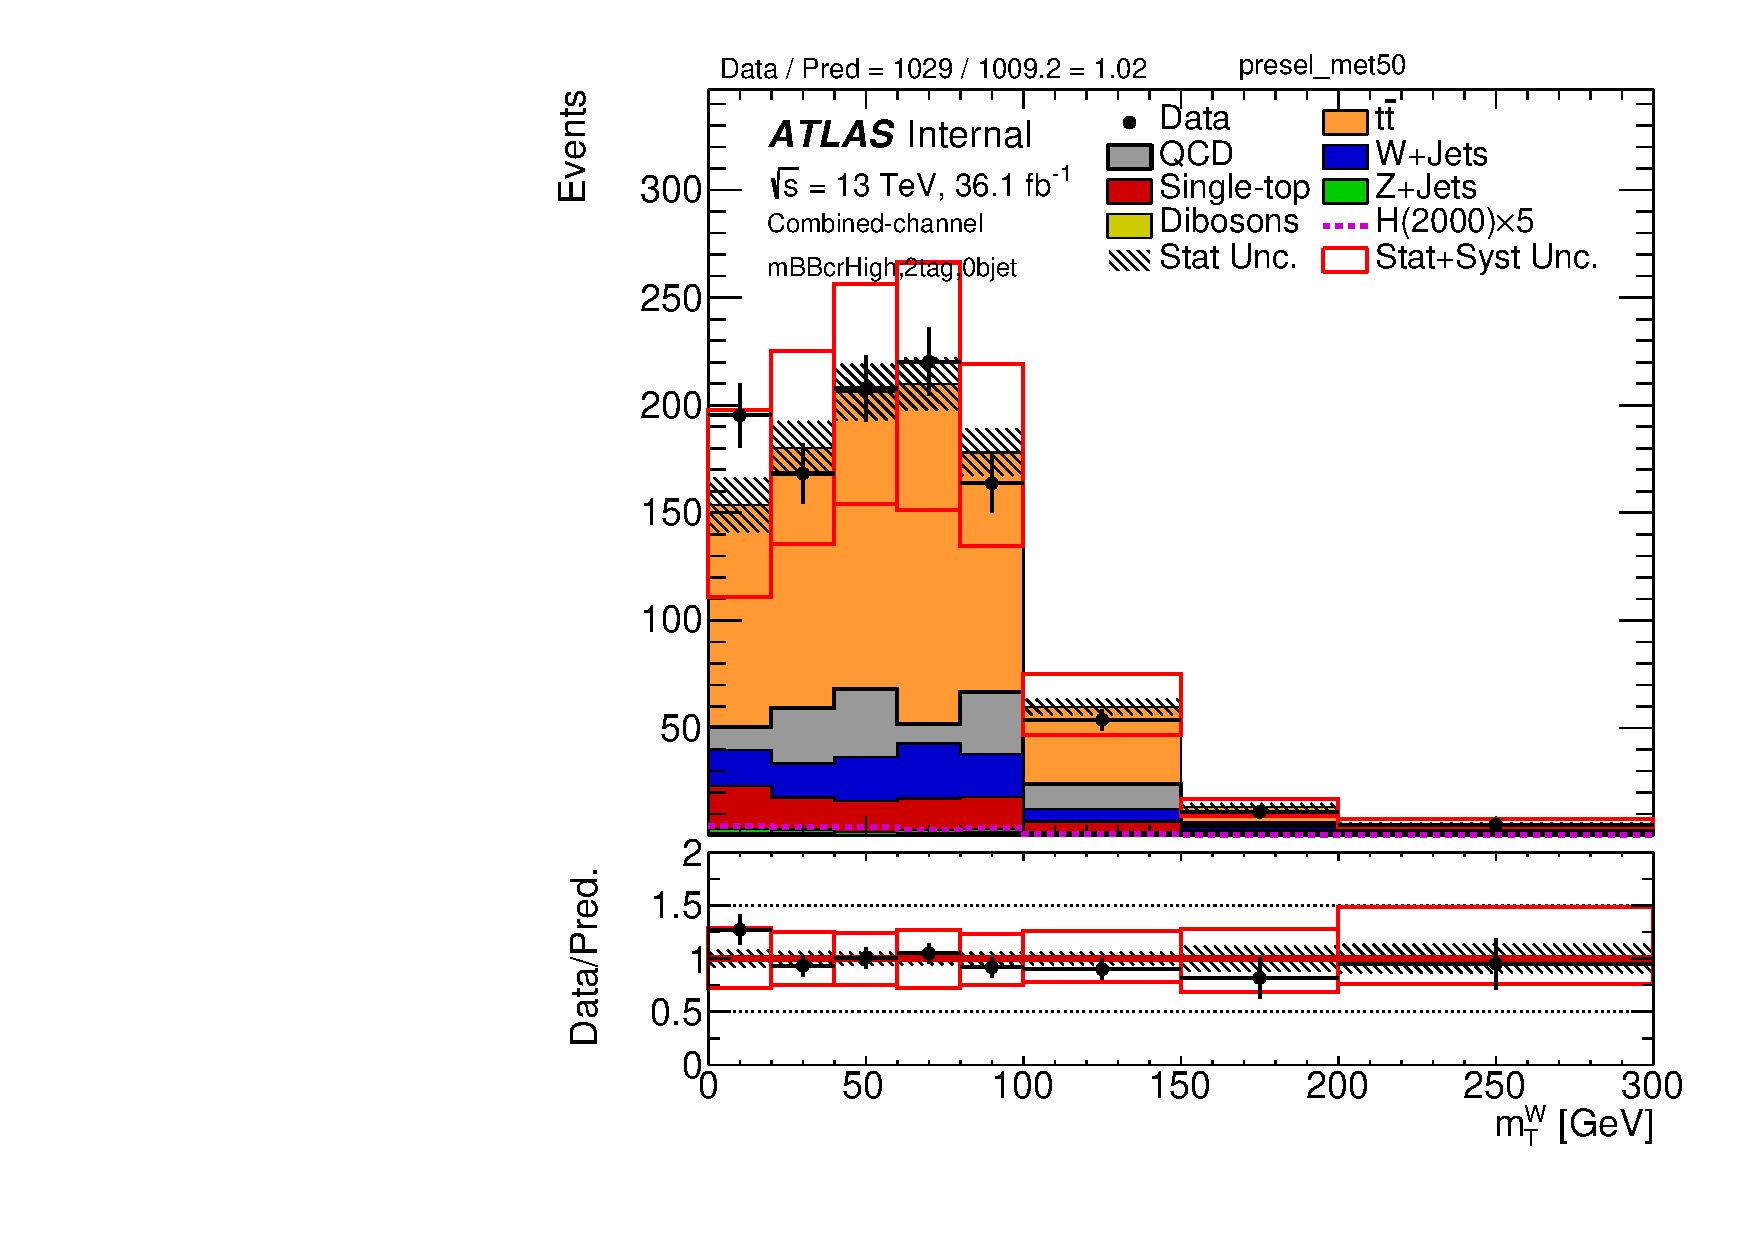
\includegraphics[scale=0.33]{./figures/boosted/PlotByMbbRegions/DataMC_2tag_0bjet_mbbcrHigh_lepton_presel_met50_WlepMtATLAS}                                                                        
\caption{The invariant mass of the reconstructed di-Higgs (hh) system, \met and transverse mass of the $W \to l\nu$ system 
distributions of events in the low (left) and high (right) mBB control region.}
\label{fig:boosted_mbbcrHighLow_mainplots}
\end{center}
\end{figure}

\begin{figure}[!h]
\begin{center}
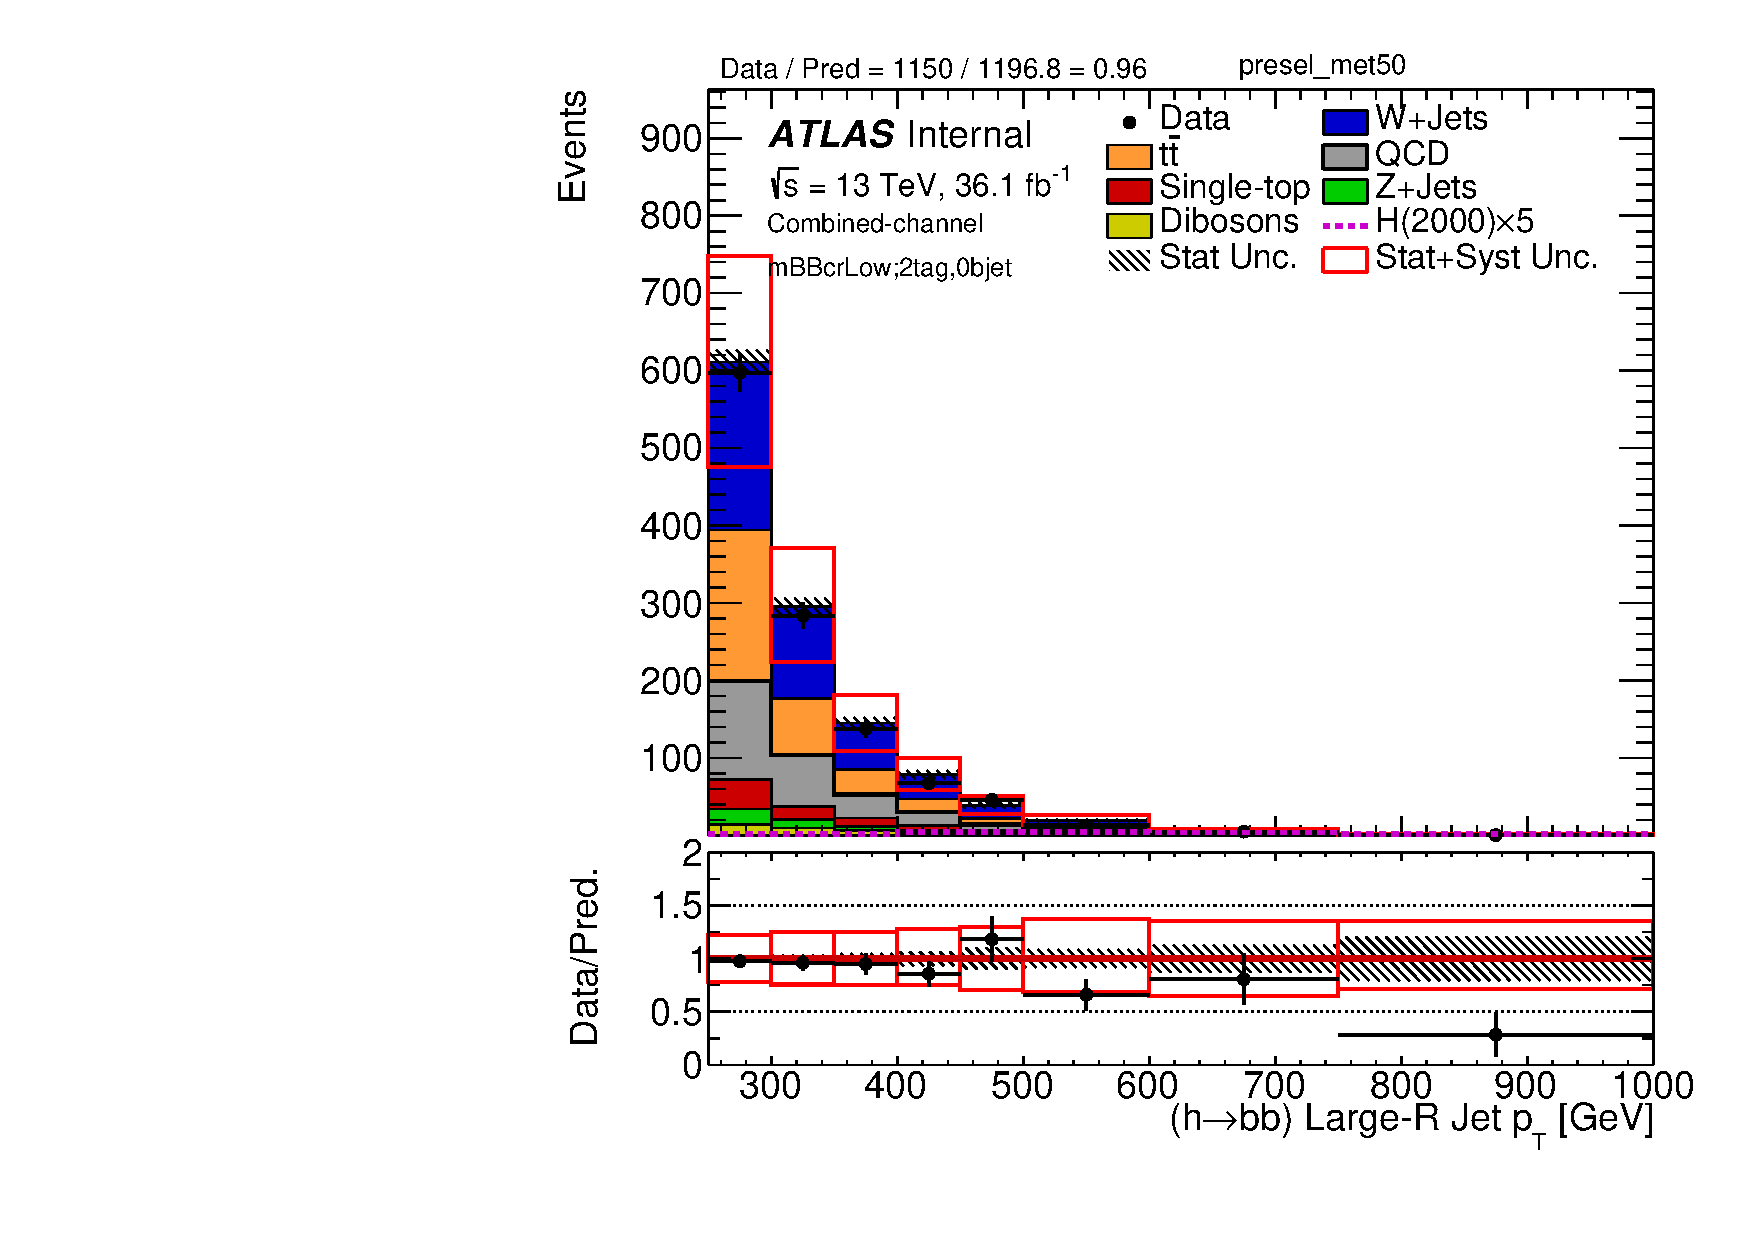
\includegraphics[scale=0.33]{./figures/boosted/PlotByMbbRegions/DataMC_2tag_0bjet_mbbcrLow_lepton_presel_met50_HbbPt}                                                                               
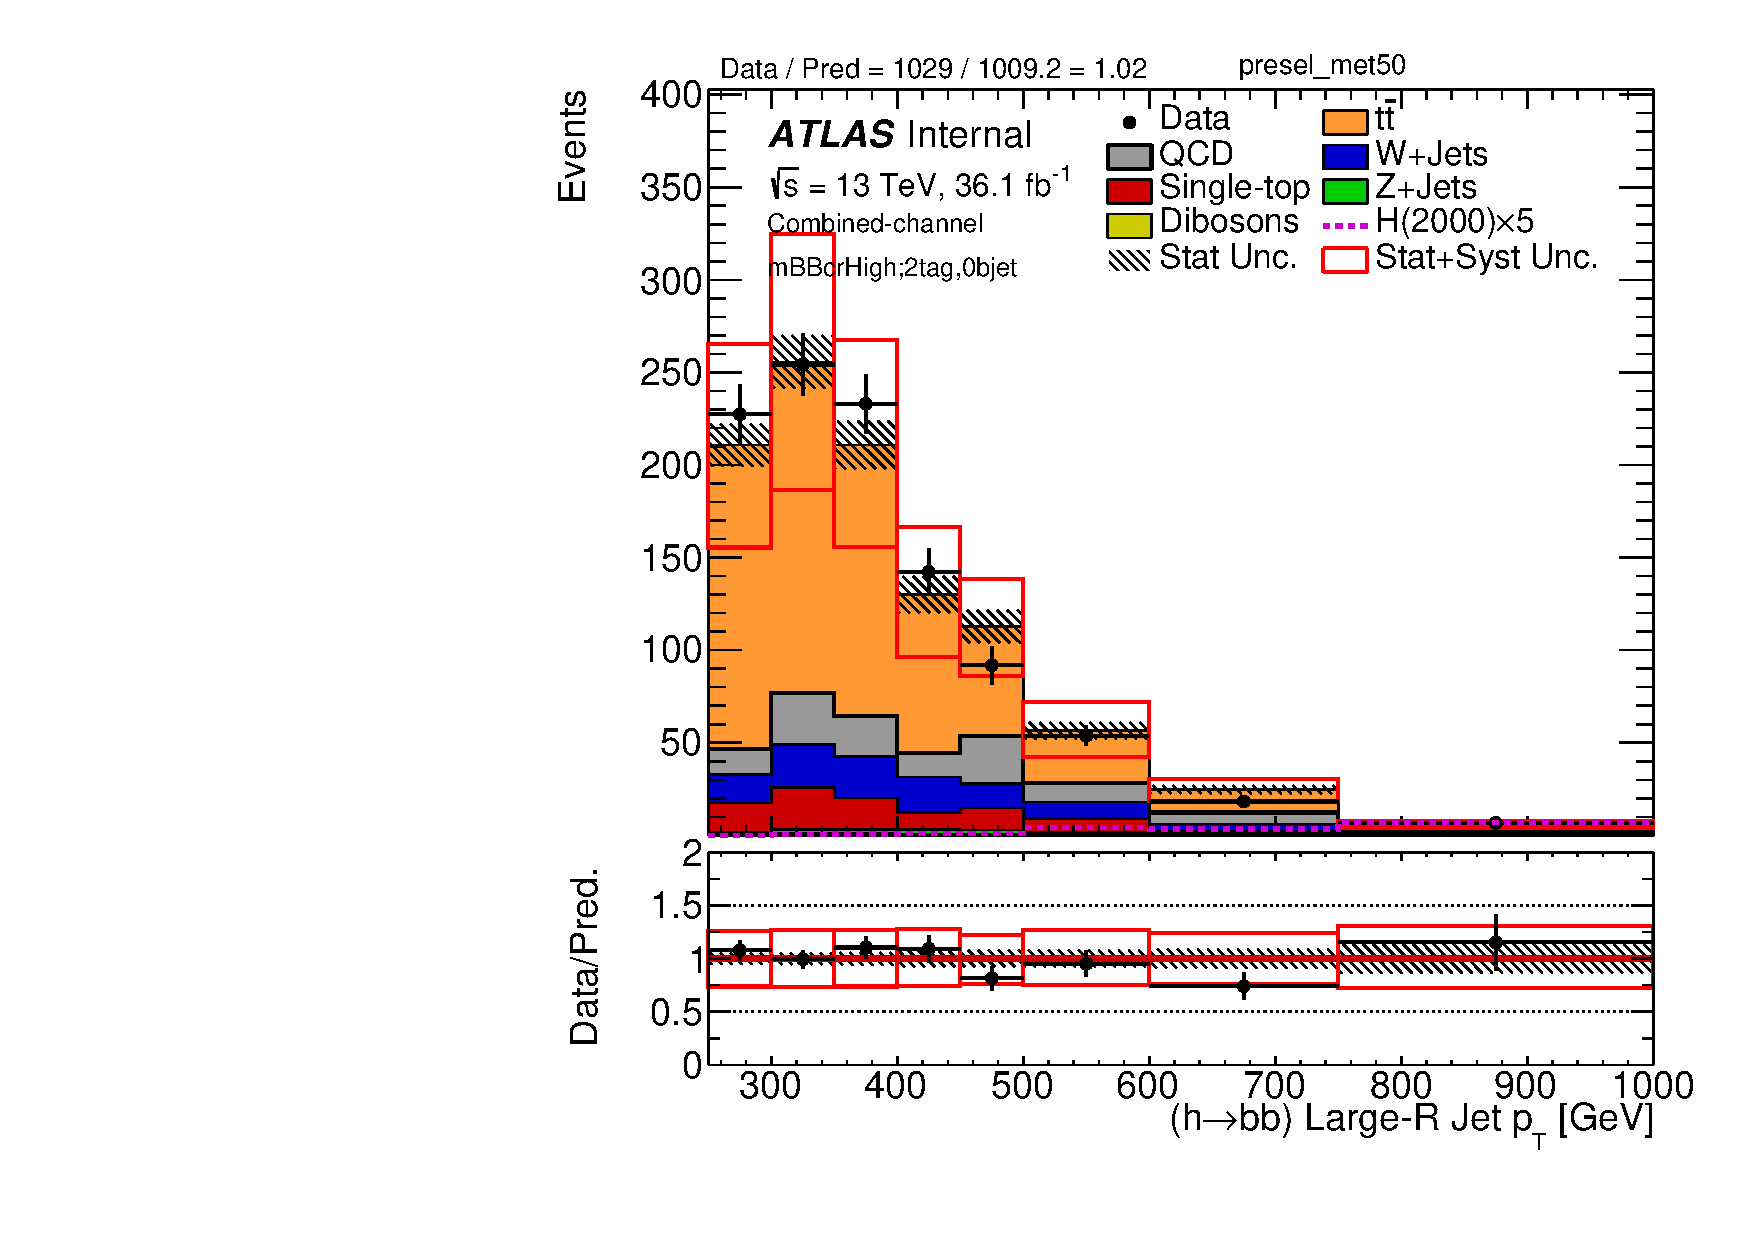
\includegraphics[scale=0.33]{./figures/boosted/PlotByMbbRegions/DataMC_2tag_0bjet_mbbcrHigh_lepton_presel_met50_HbbPt}                                                                              
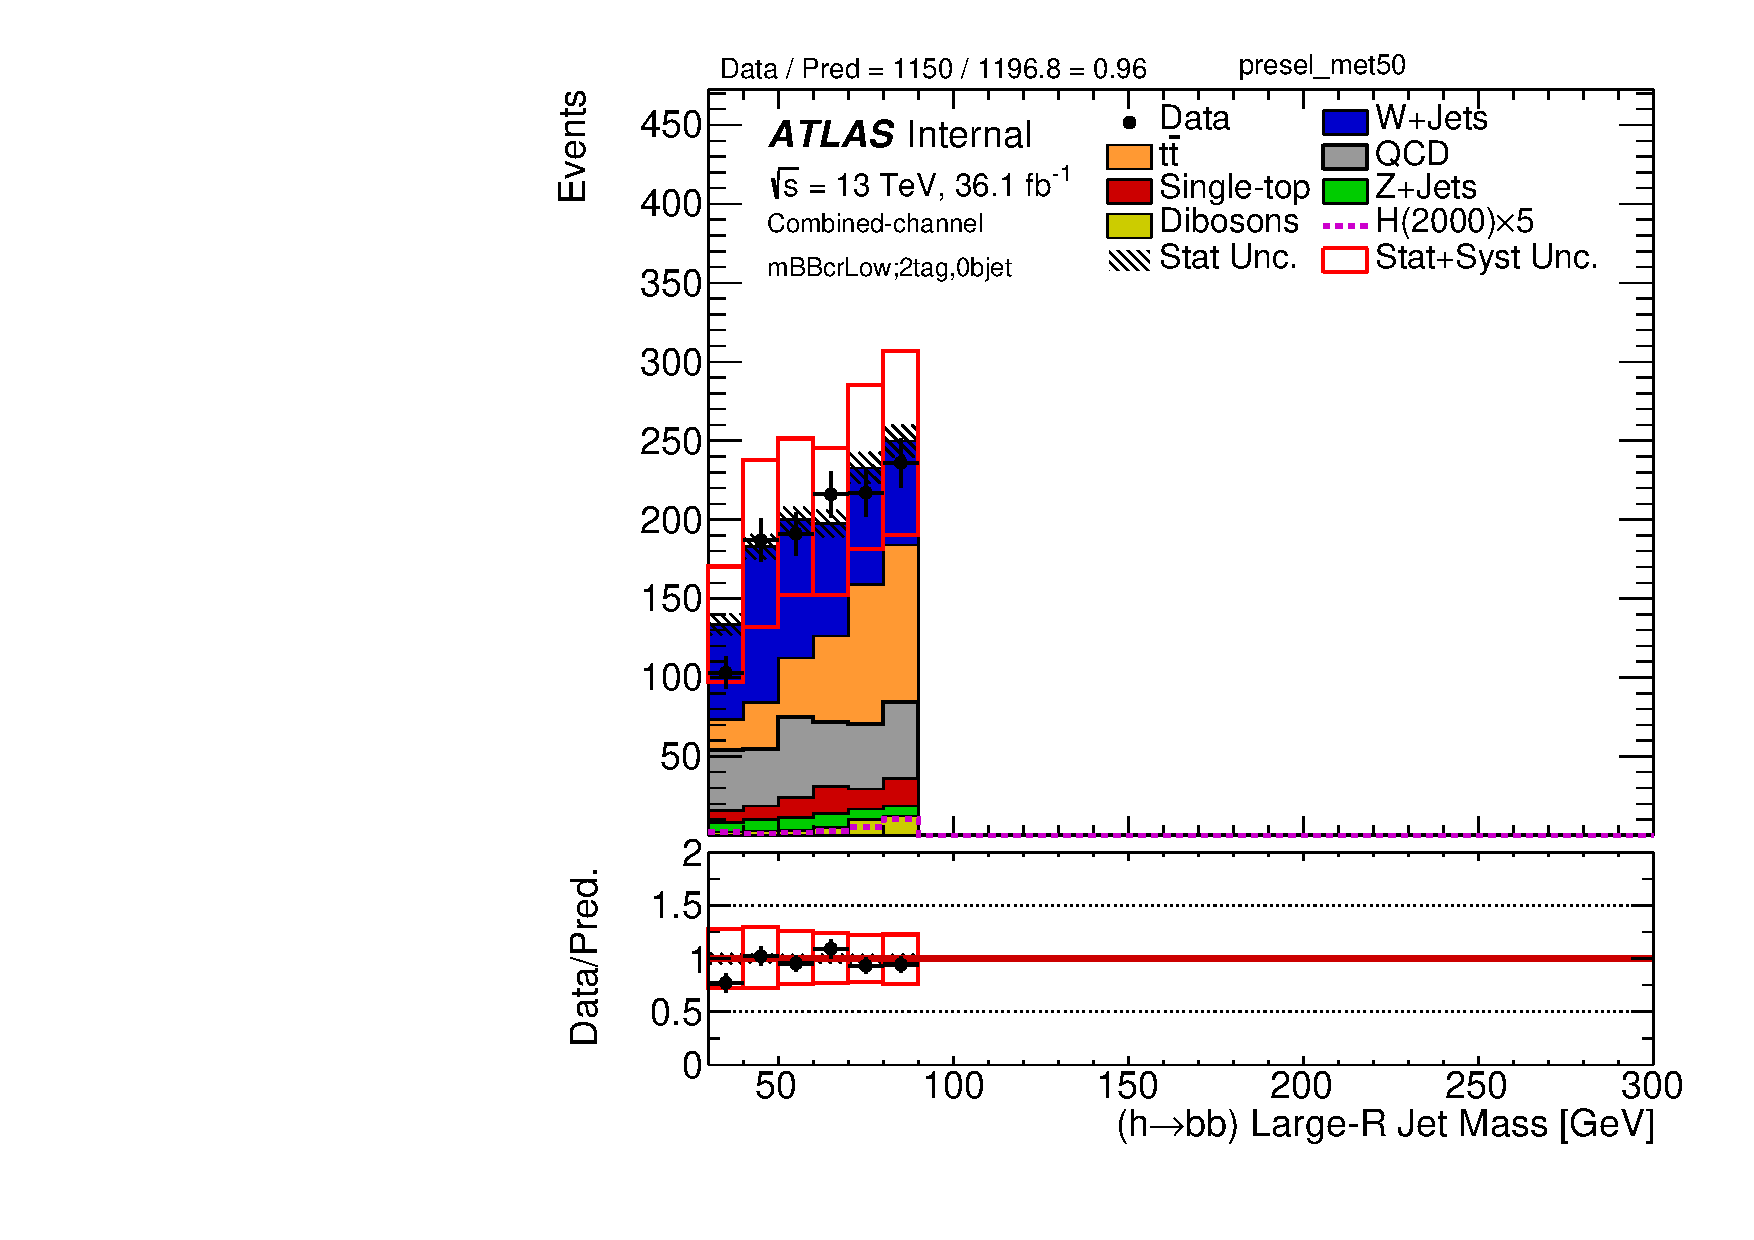
\includegraphics[scale=0.33]{./figures/boosted/PlotByMbbRegions/DataMC_2tag_0bjet_mbbcrLow_lepton_presel_met50_HbbMass}                                                                             
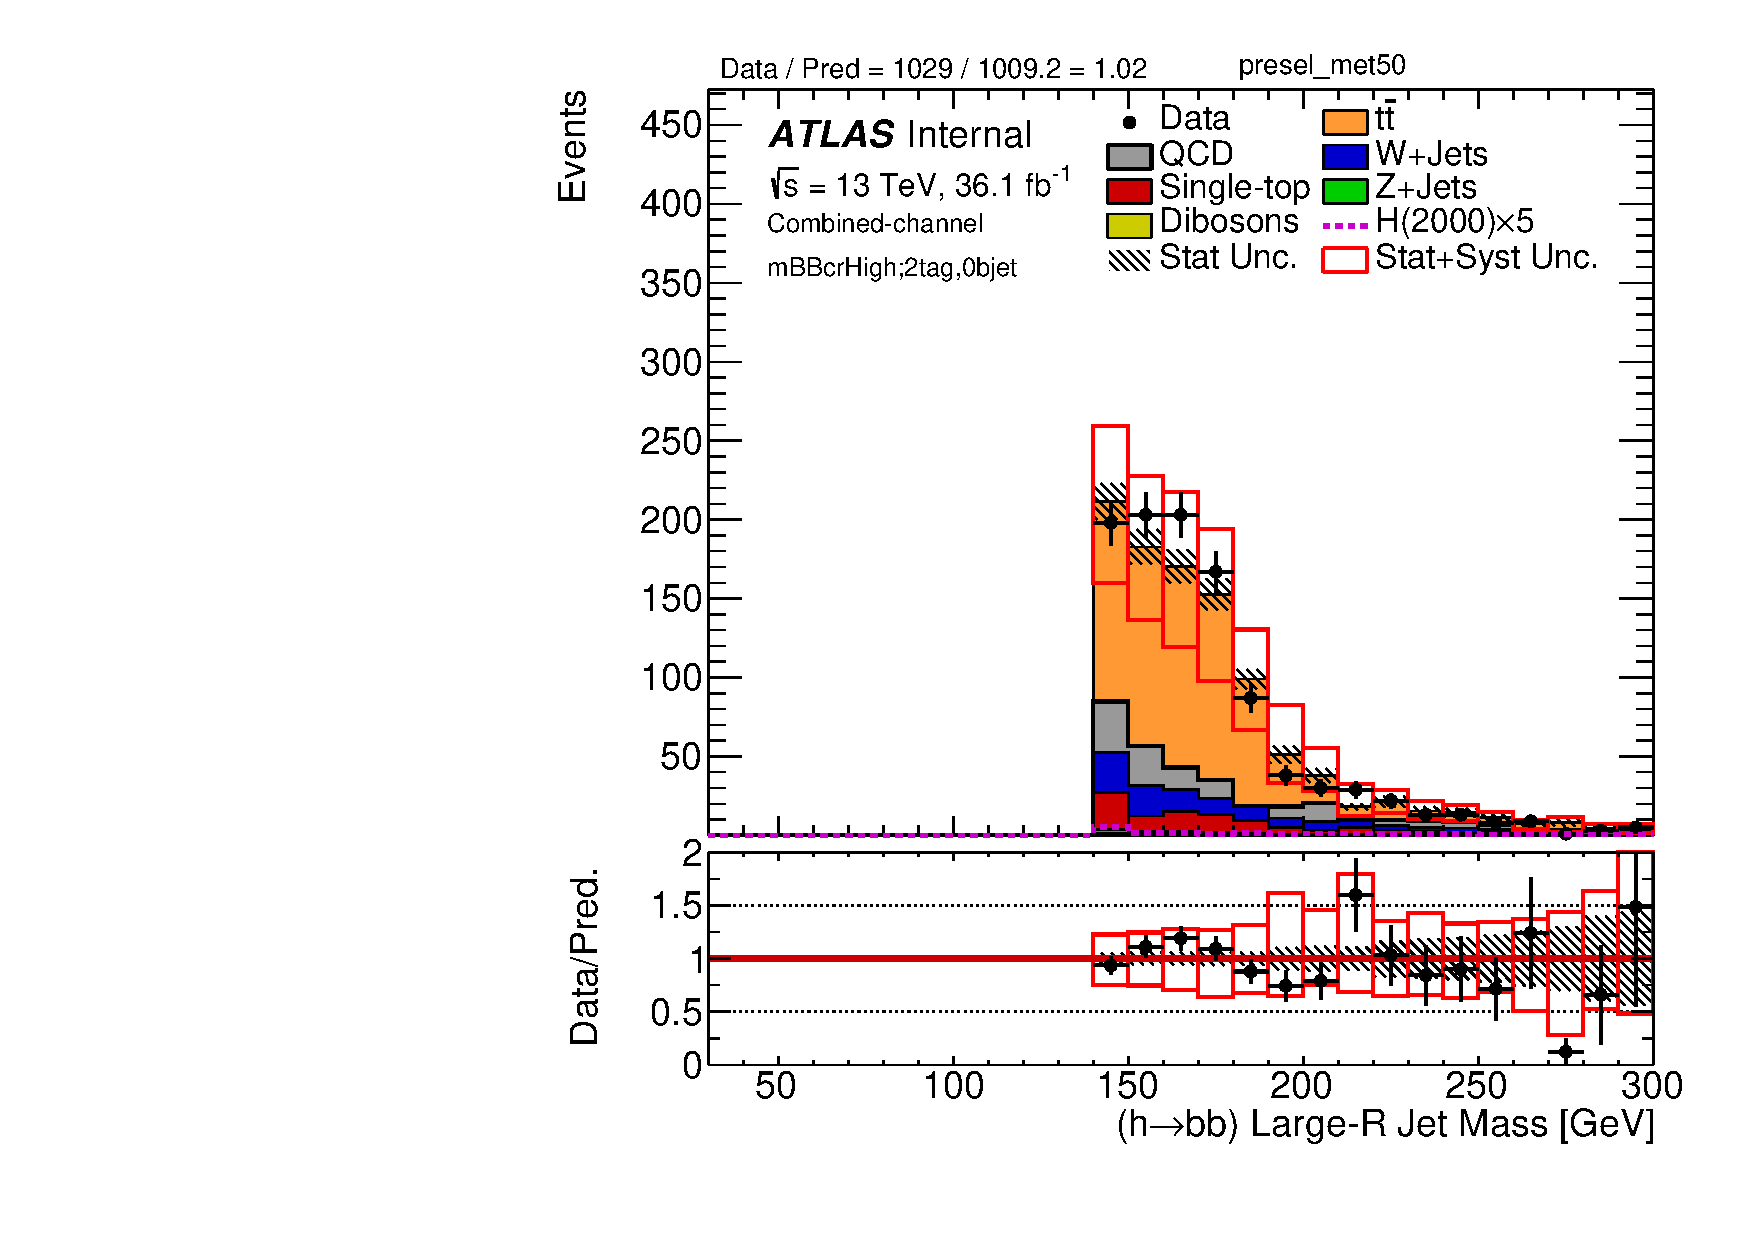
\includegraphics[scale=0.33]{./figures/boosted/PlotByMbbRegions/DataMC_2tag_0bjet_mbbcrHigh_lepton_presel_met50_HbbMass}                                                                            
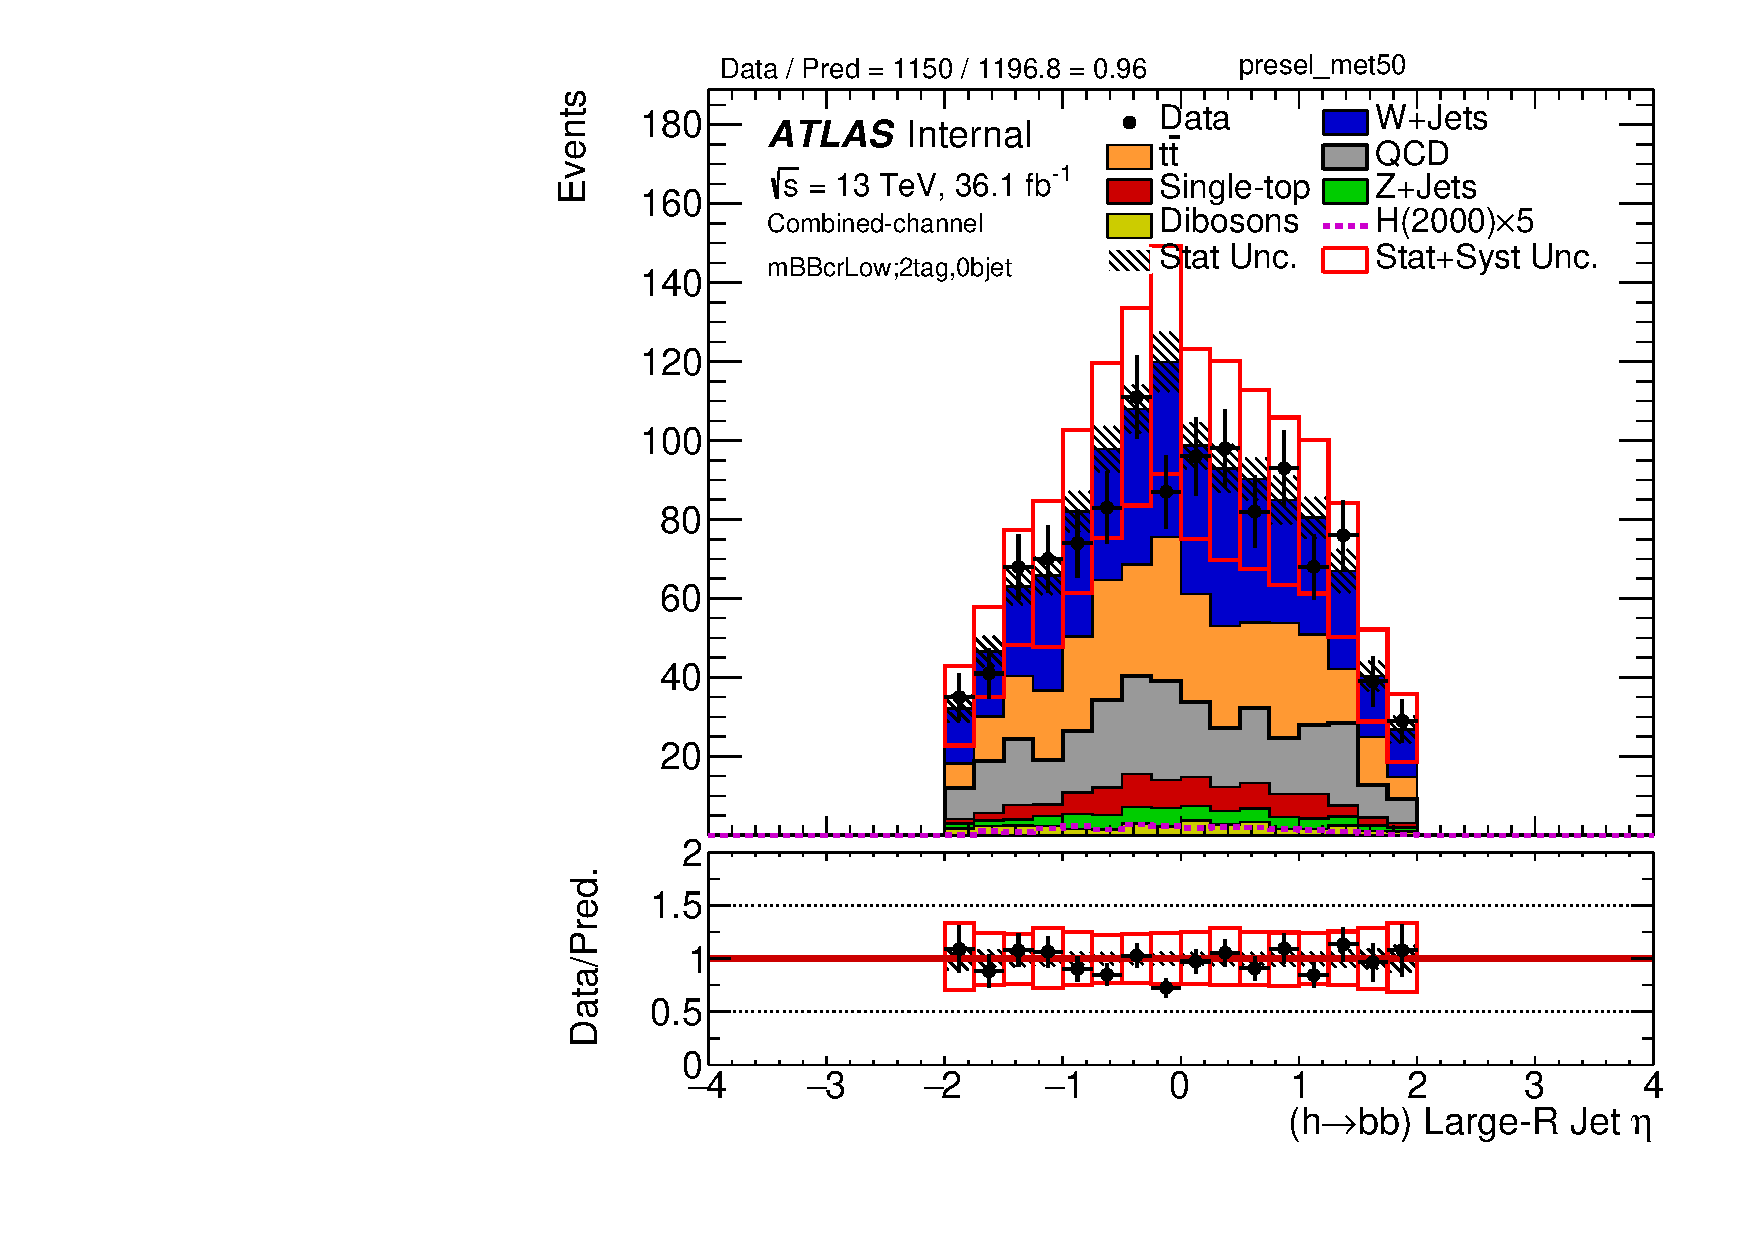
\includegraphics[scale=0.33]{./figures/boosted/PlotByMbbRegions/DataMC_2tag_0bjet_mbbcrLow_lepton_presel_met50_HbbEta}
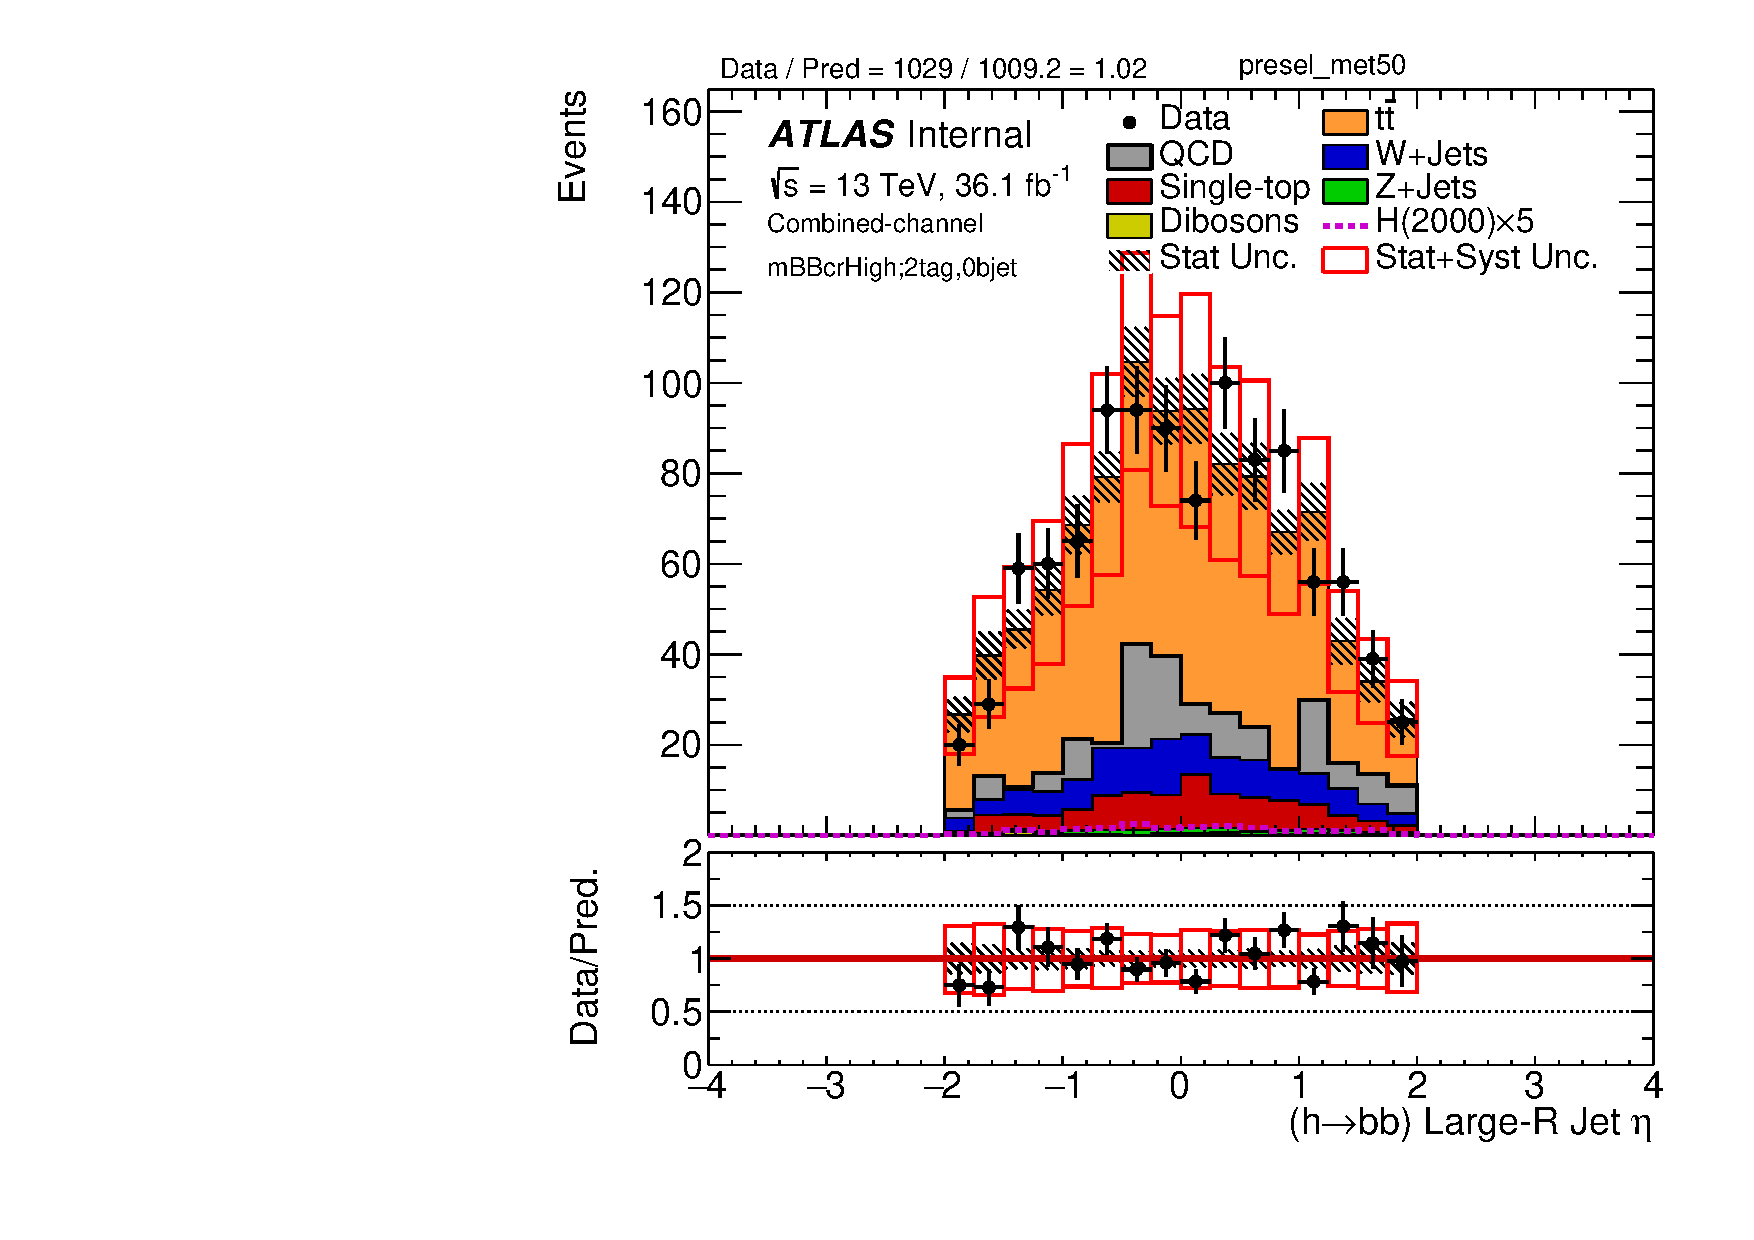
\includegraphics[scale=0.33]{./figures/boosted/PlotByMbbRegions/DataMC_2tag_0bjet_mbbcrHigh_lepton_presel_met50_HbbEta}                                                                             
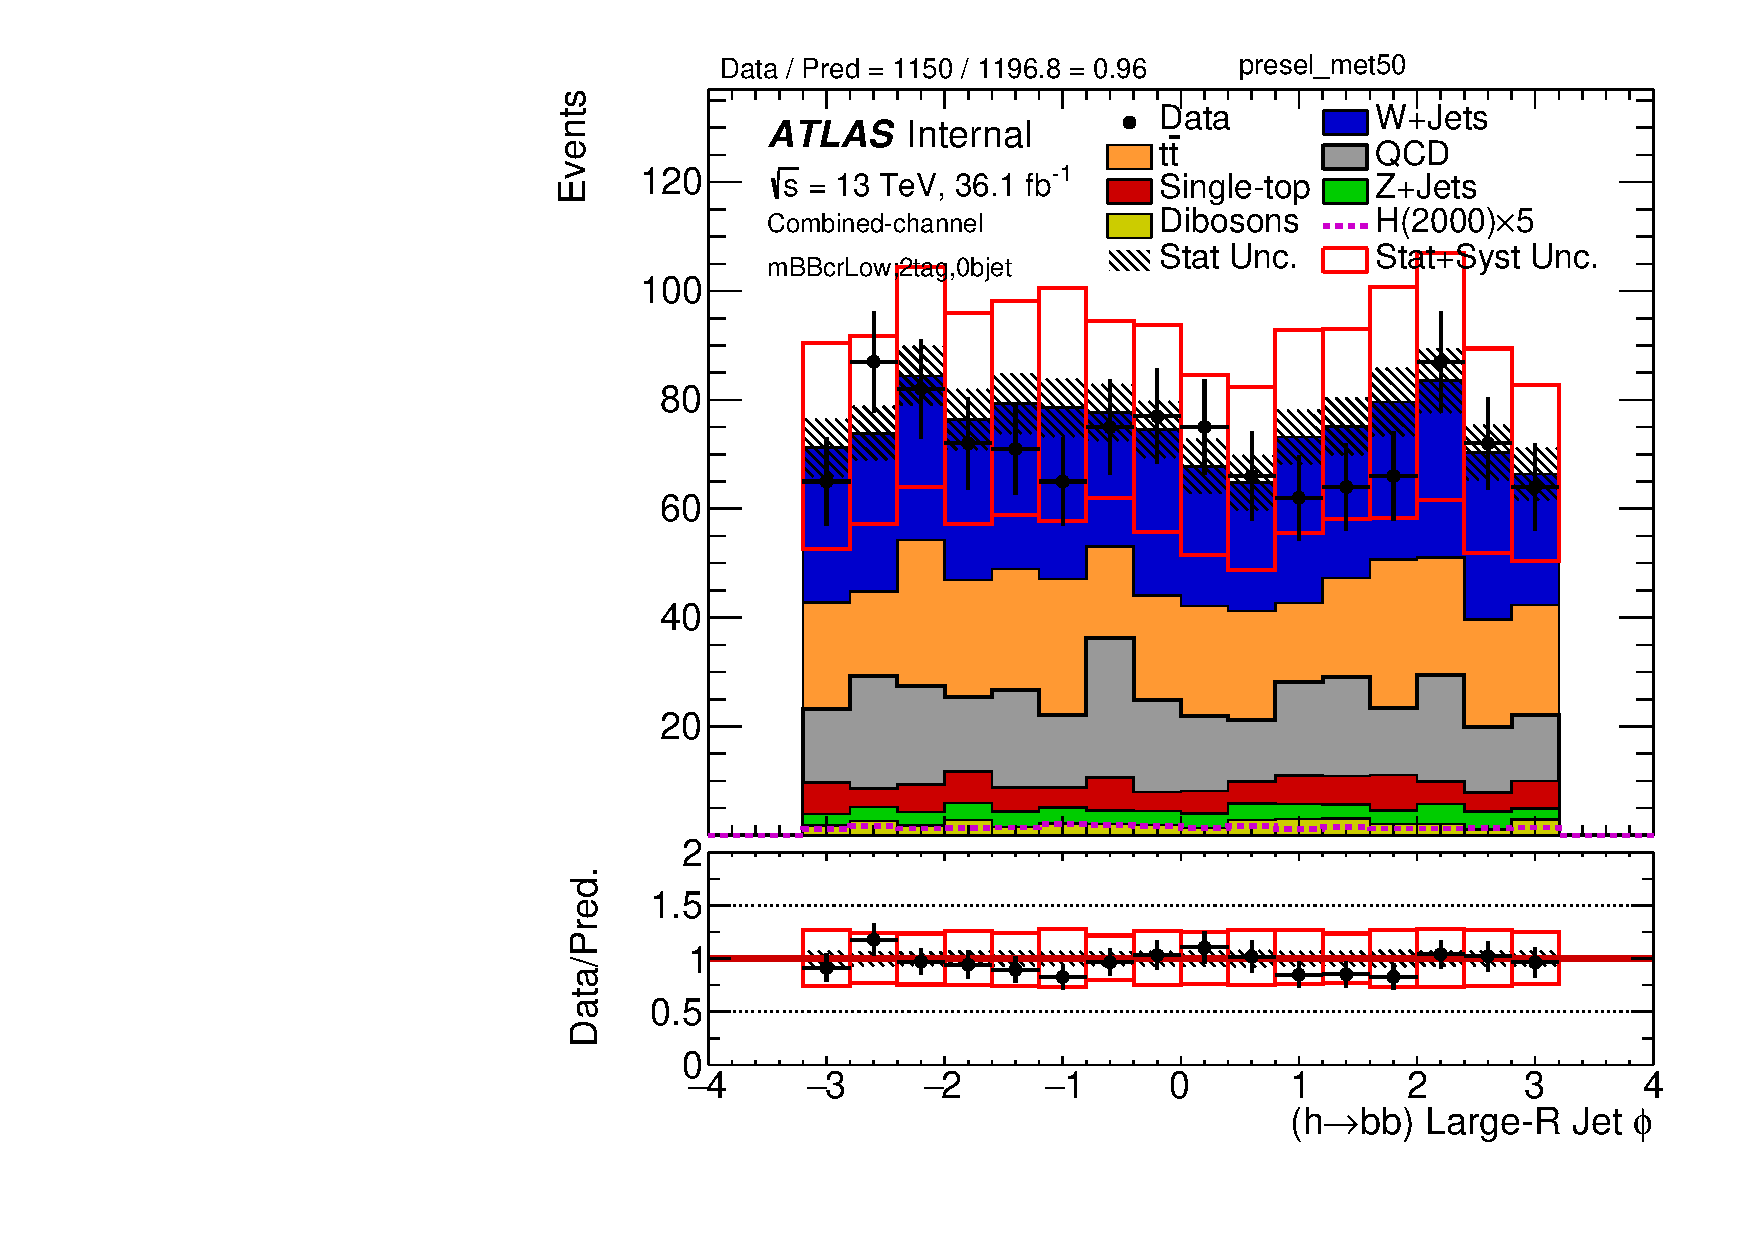
\includegraphics[scale=0.33]{./figures/boosted/PlotByMbbRegions/DataMC_2tag_0bjet_mbbcrLow_lepton_presel_met50_HbbPhi} 
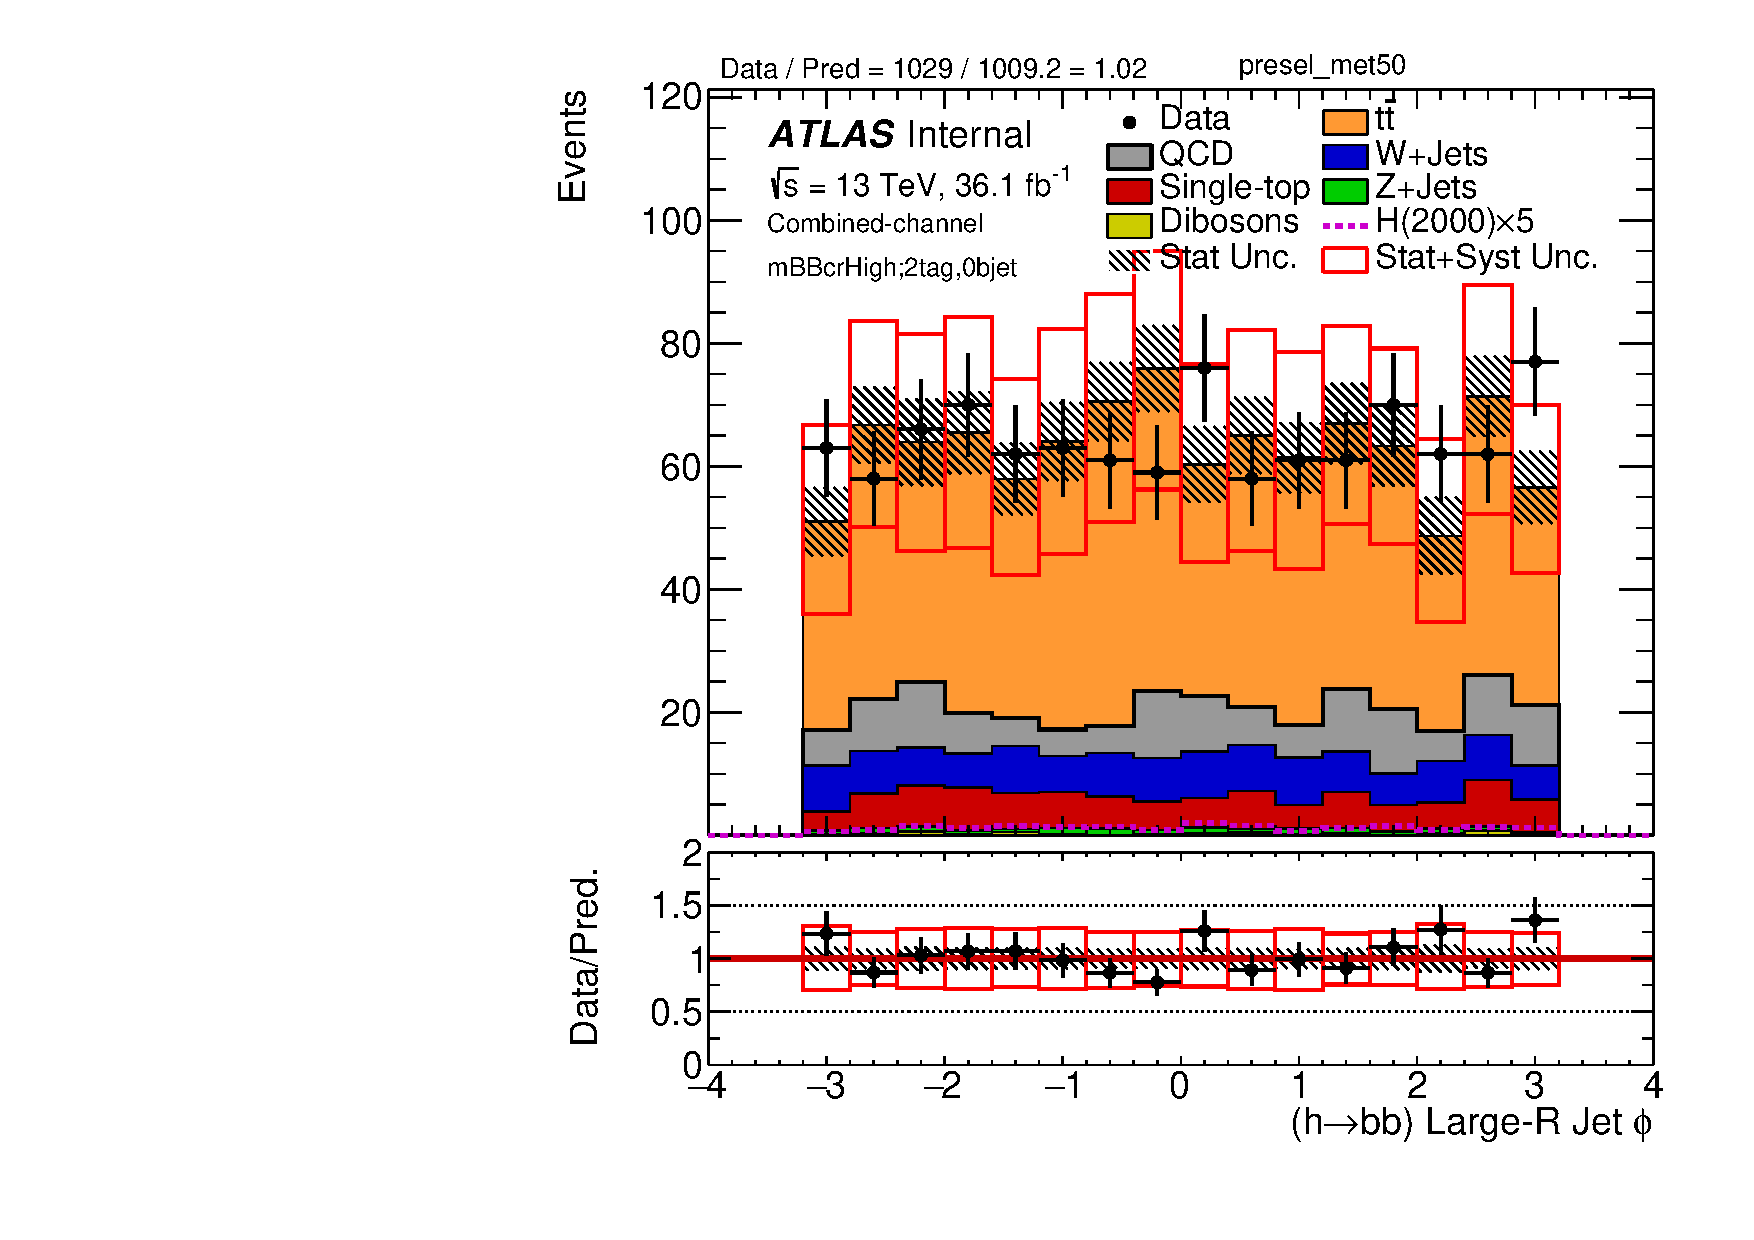
\includegraphics[scale=0.33]{./figures/boosted/PlotByMbbRegions/DataMC_2tag_0bjet_mbbcrHigh_lepton_presel_met50_HbbPhi}                                                                             
\caption{Kinematic distributions of the reconstructed large-$R$ jet in the low (left) and high (right) mBB control region.}
\label{fig:boosted_mbbcrHighLow_largerjet}
\end{center}
\end{figure}

\begin{figure}[!h]
\begin{center}
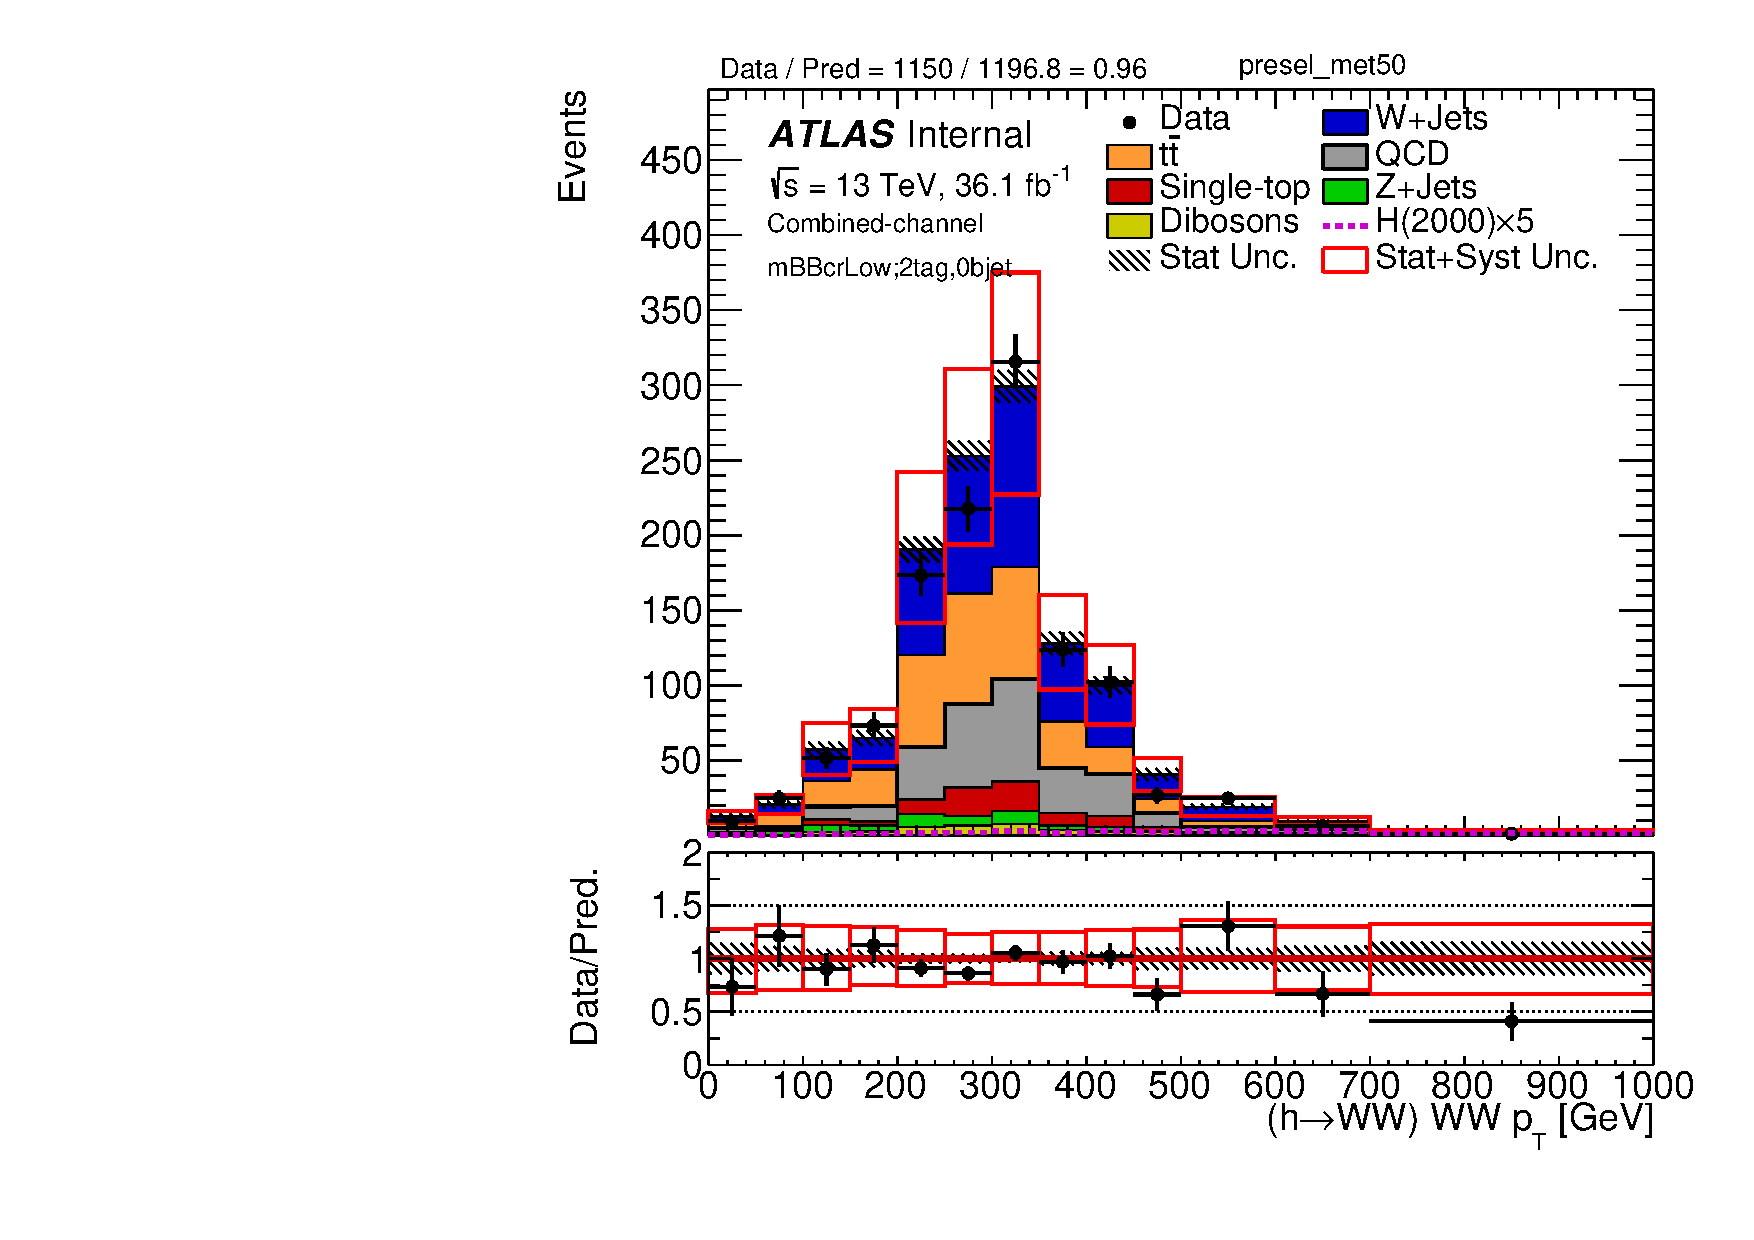
\includegraphics[scale=0.33]{./figures/boosted/PlotByMbbRegions/DataMC_2tag_0bjet_mbbcrLow_lepton_presel_met50_WWPt}                                                                                
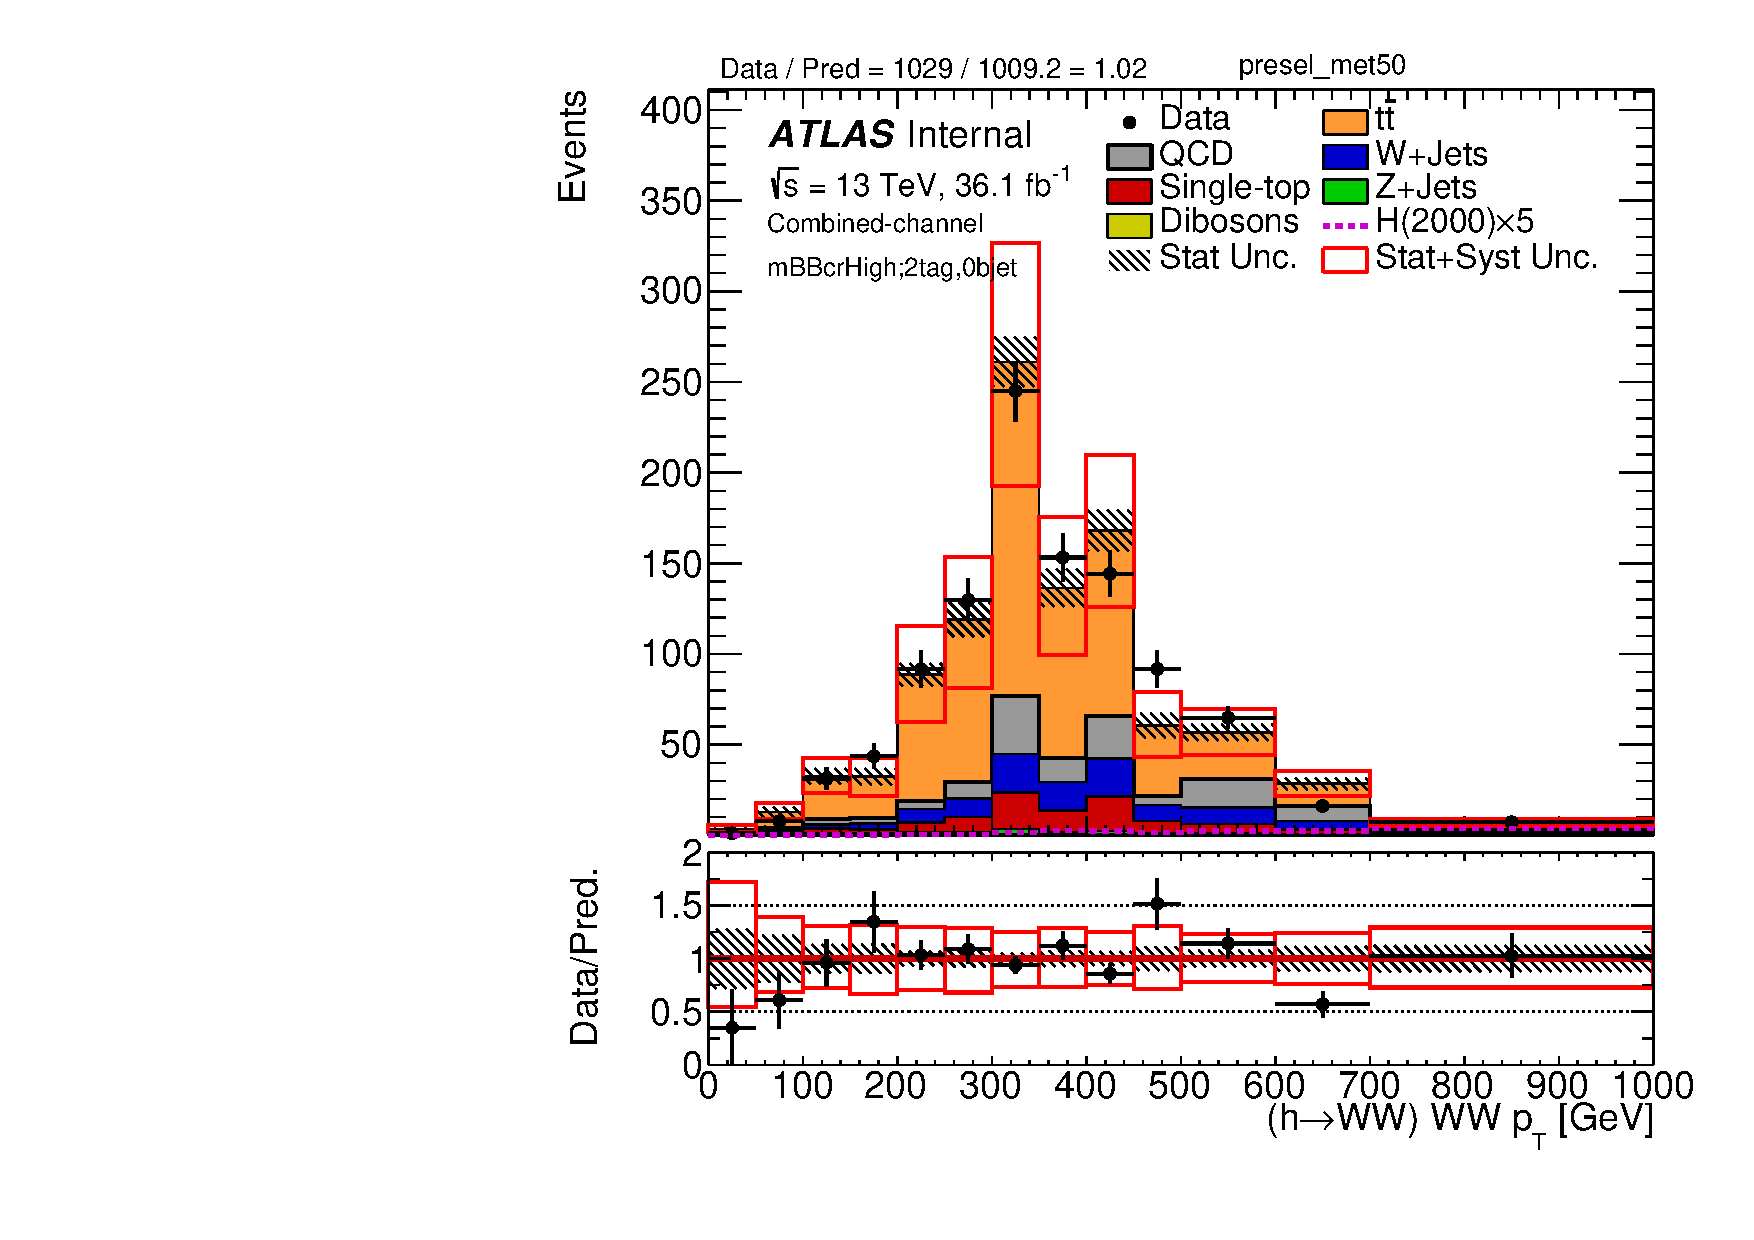
\includegraphics[scale=0.33]{./figures/boosted/PlotByMbbRegions/DataMC_2tag_0bjet_mbbcrHigh_lepton_presel_met50_WWPt}                                                                               
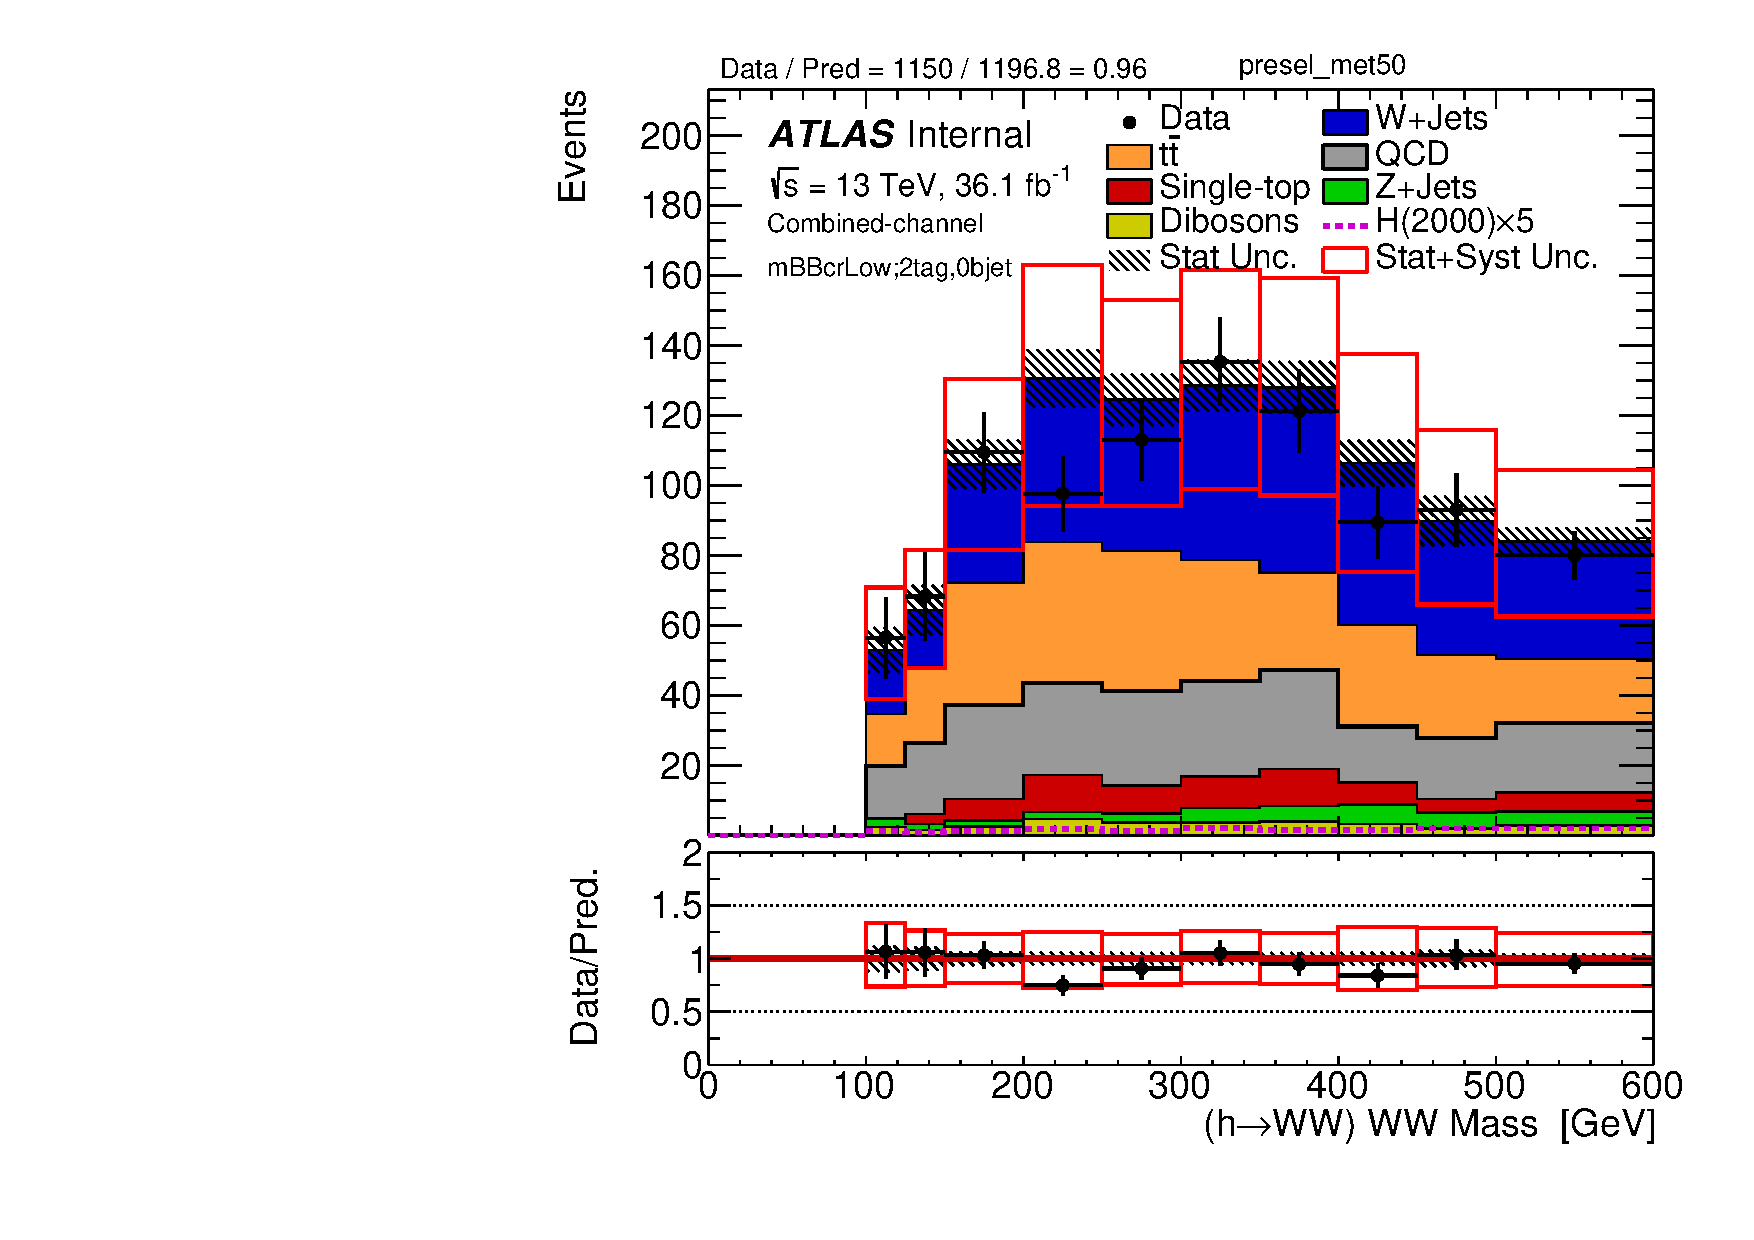
\includegraphics[scale=0.33]{./figures/boosted/PlotByMbbRegions/DataMC_2tag_0bjet_mbbcrLow_lepton_presel_met50_WWMass}                                                                              
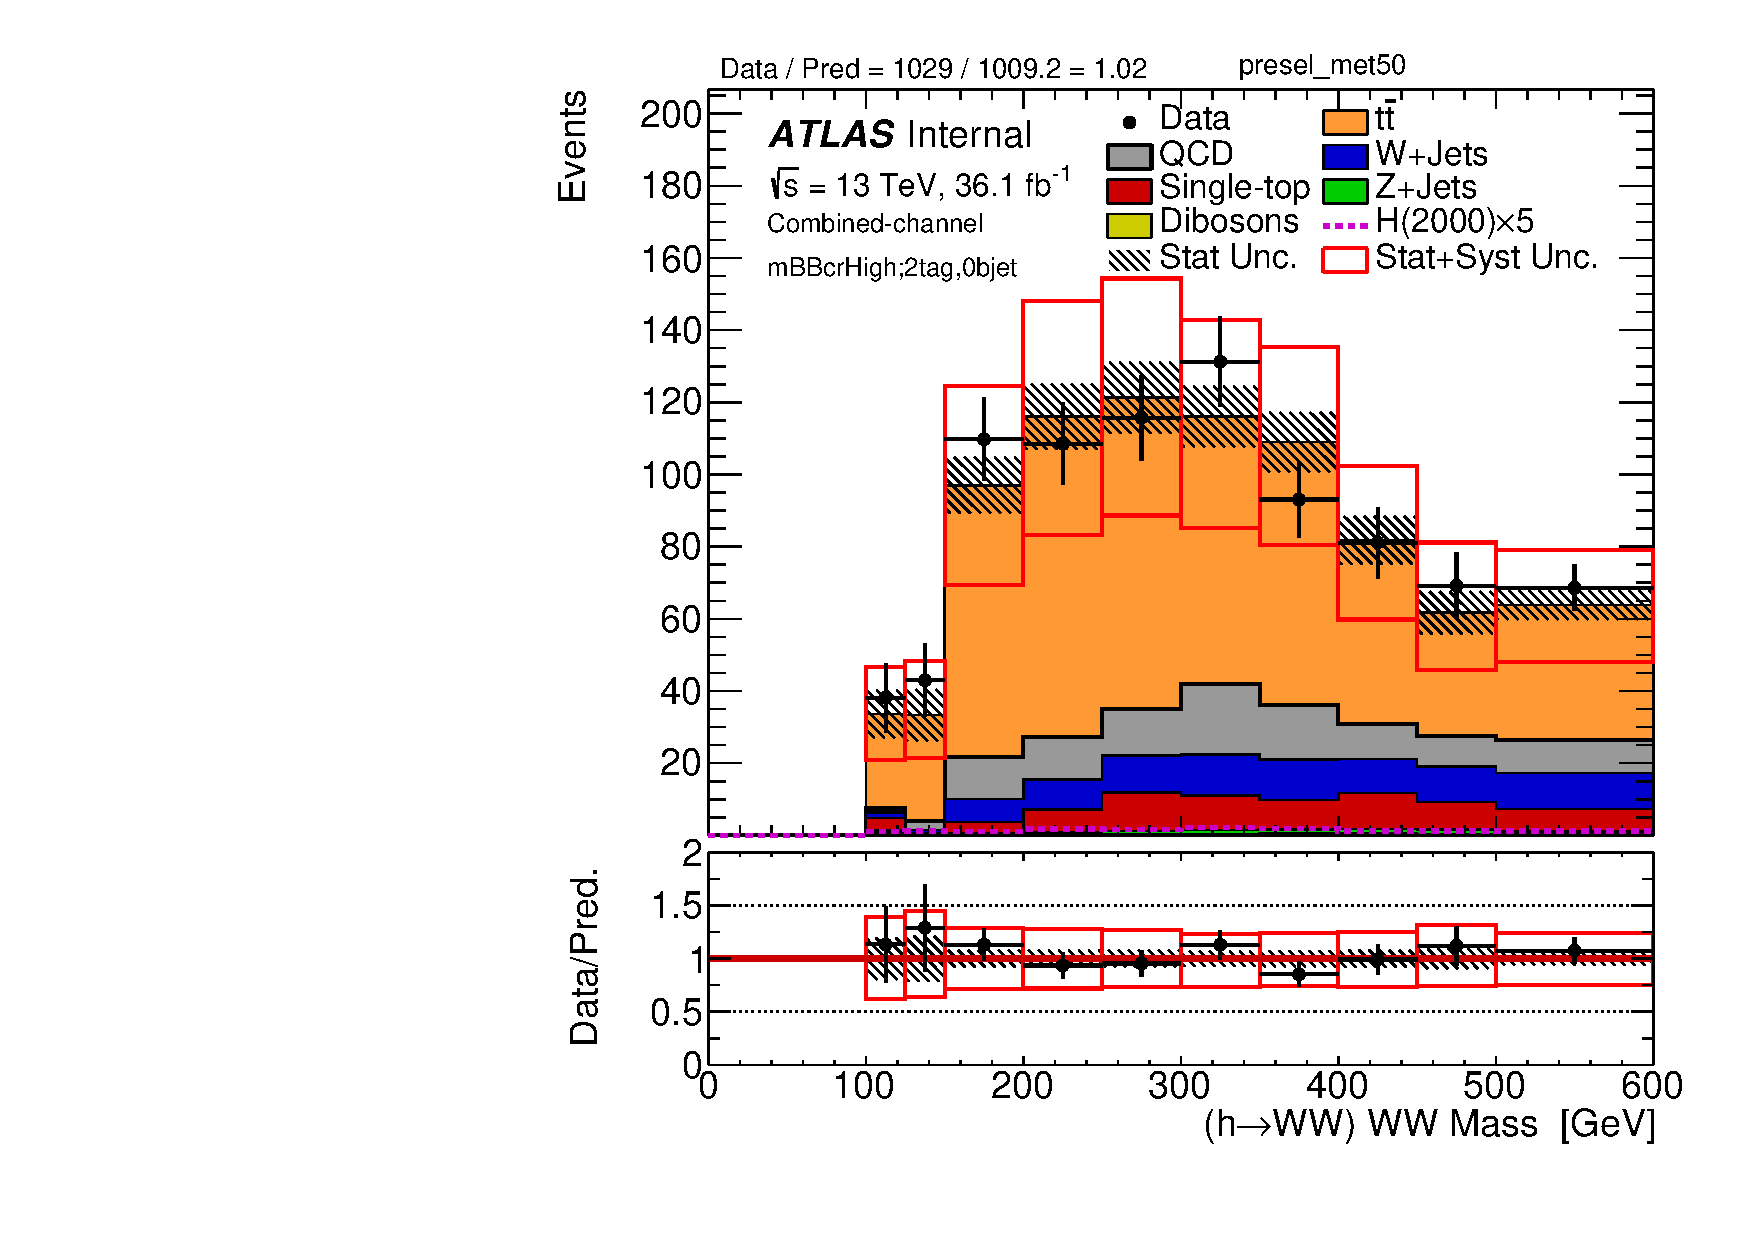
\includegraphics[scale=0.33]{./figures/boosted/PlotByMbbRegions/DataMC_2tag_0bjet_mbbcrHigh_lepton_presel_met50_WWMass}                                                                             
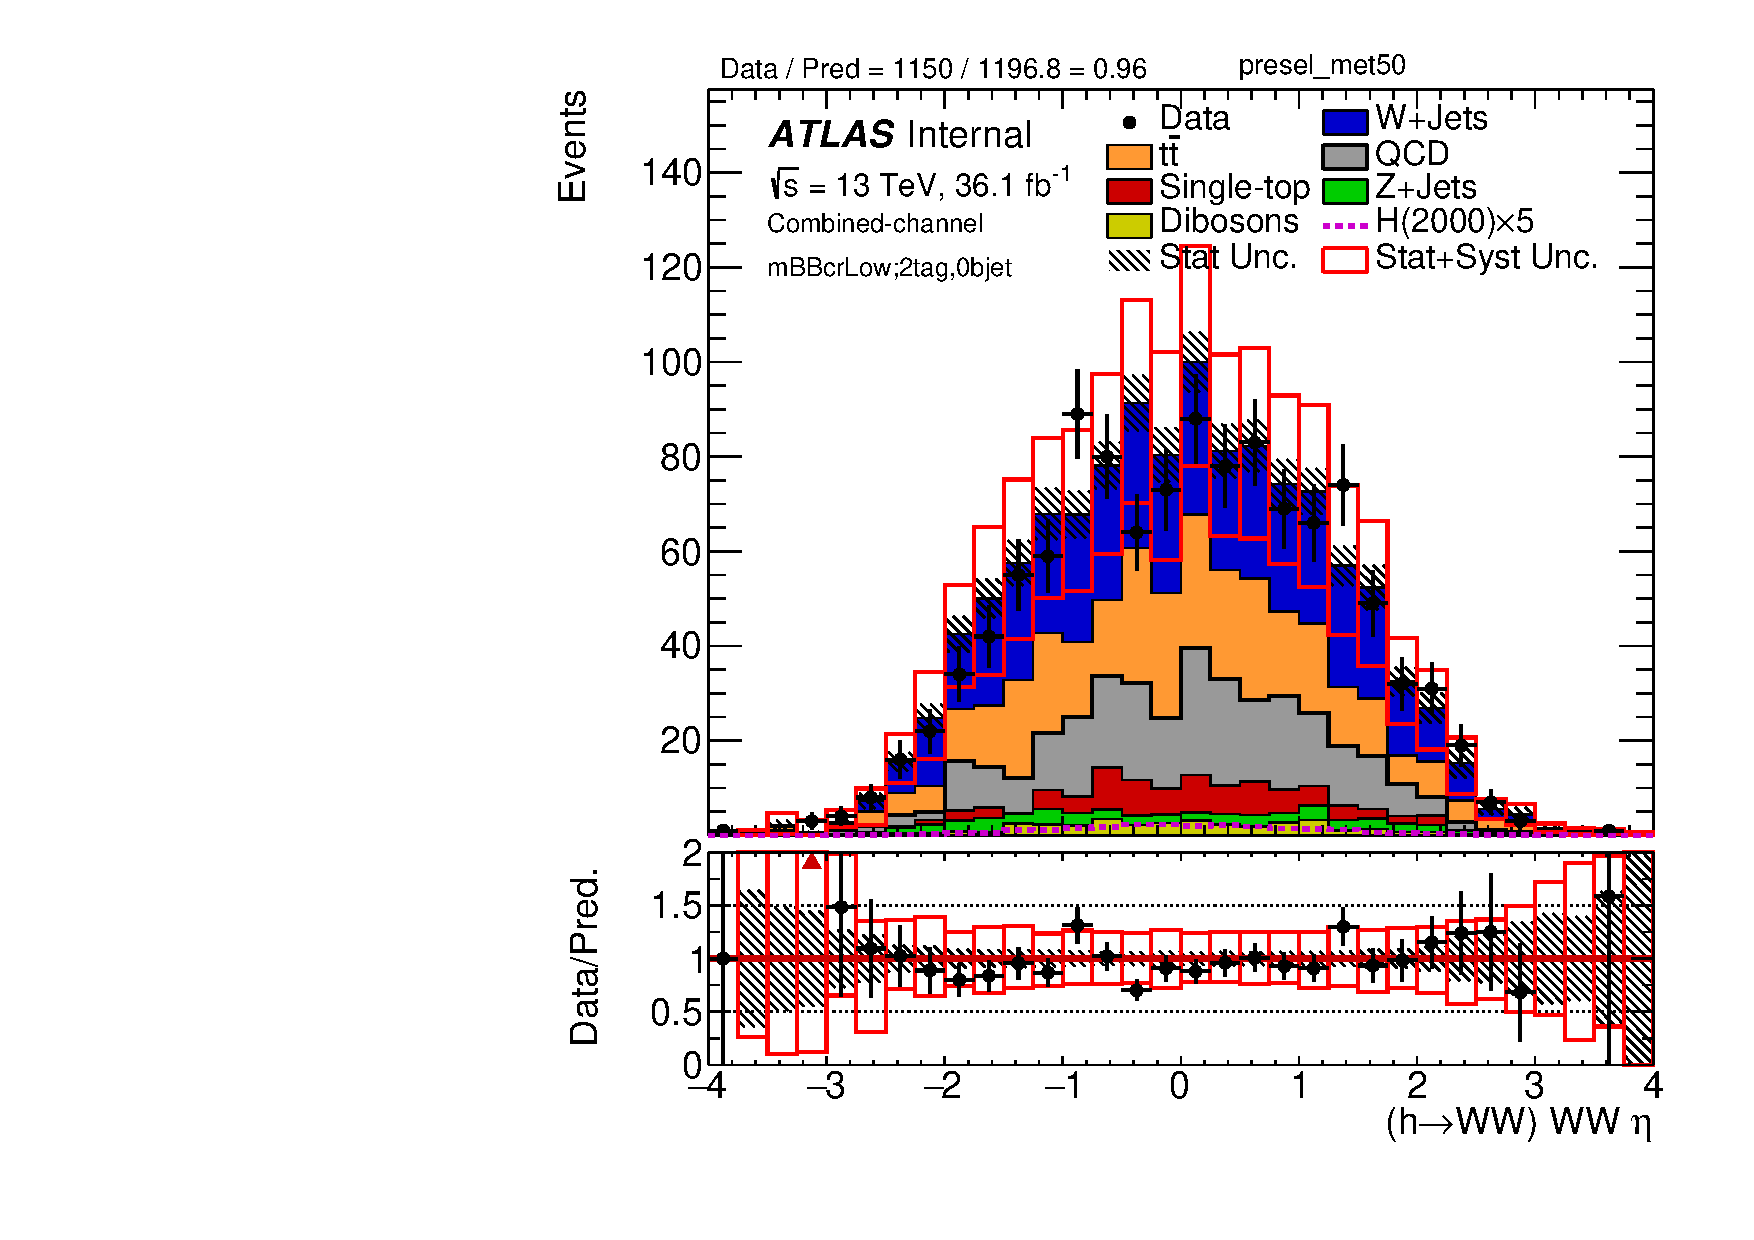
\includegraphics[scale=0.33]{./figures/boosted/PlotByMbbRegions/DataMC_2tag_0bjet_mbbcrLow_lepton_presel_met50_WWEta}                                                                               
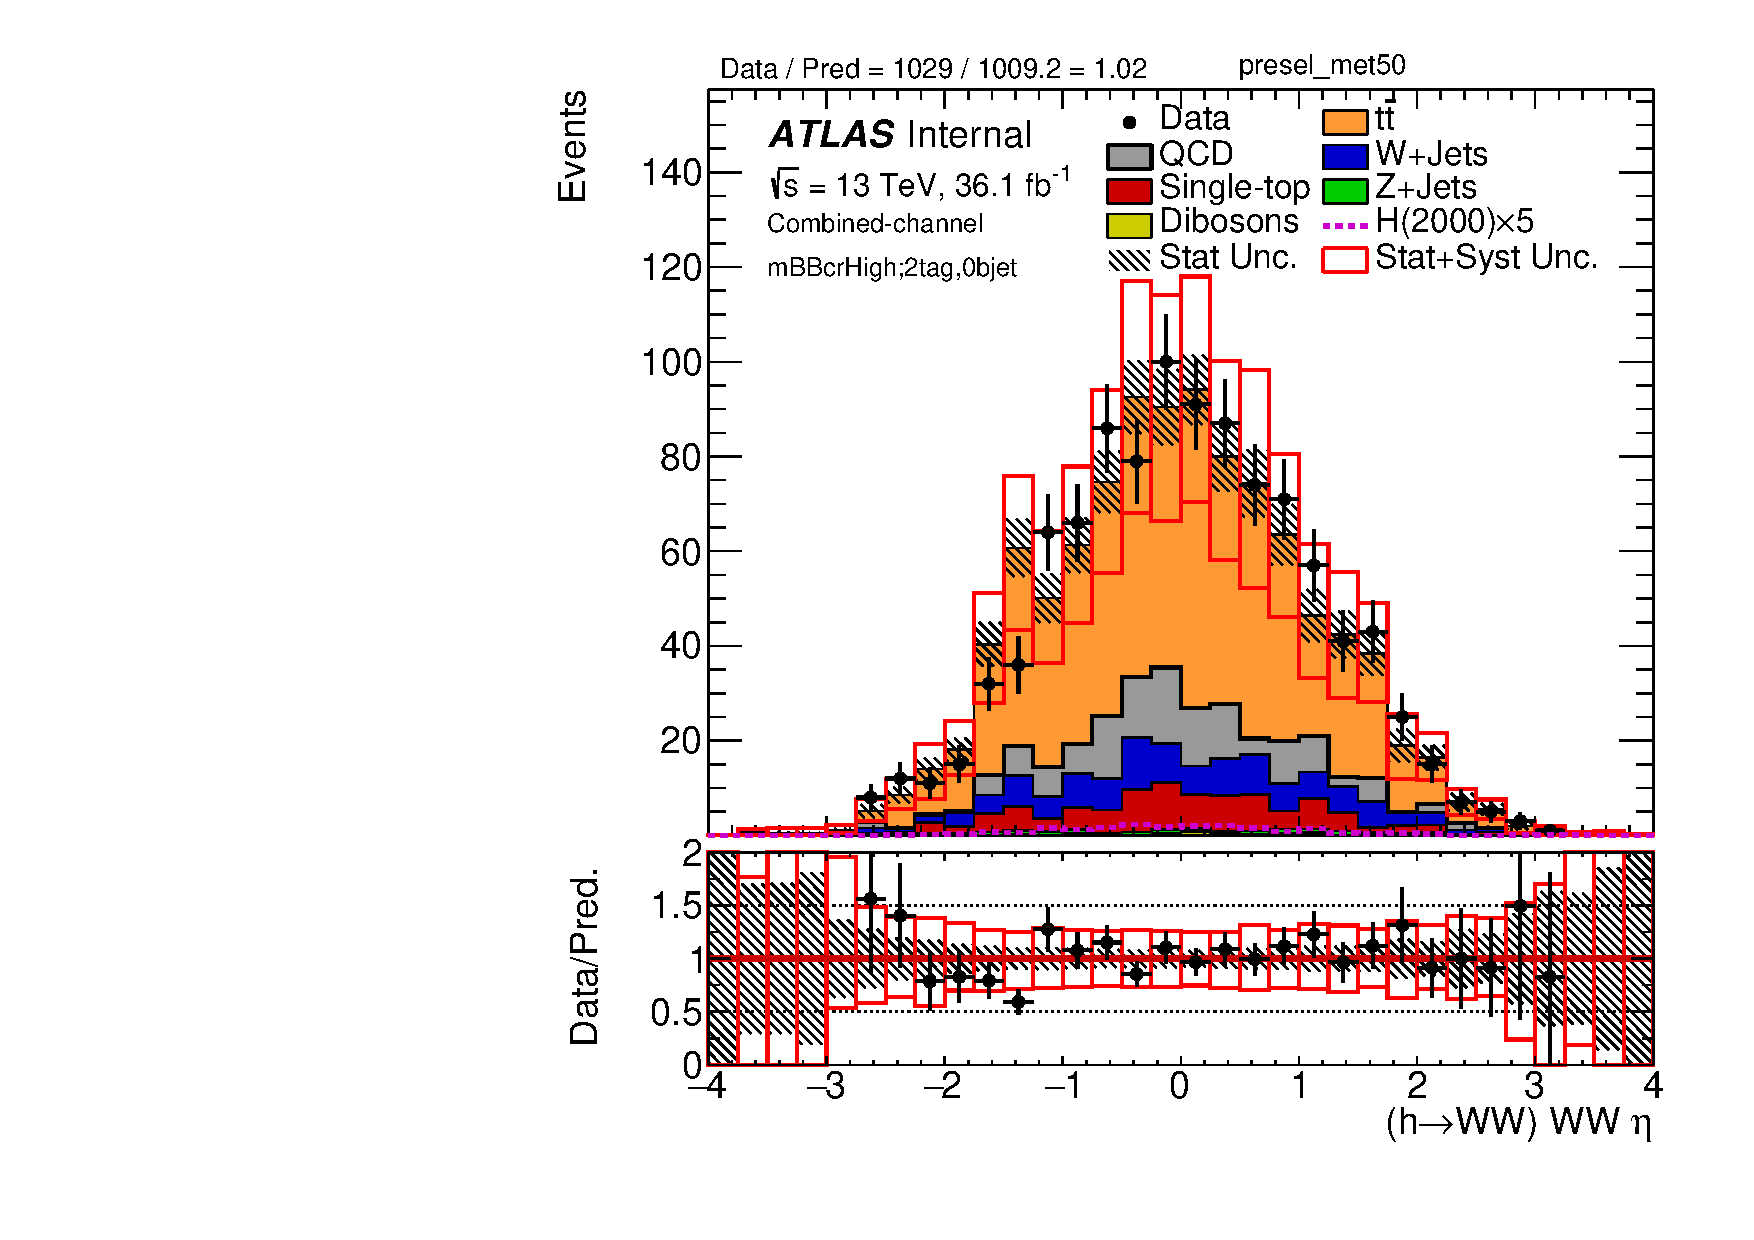
\includegraphics[scale=0.33]{./figures/boosted/PlotByMbbRegions/DataMC_2tag_0bjet_mbbcrHigh_lepton_presel_met50_WWEta}                                                                              
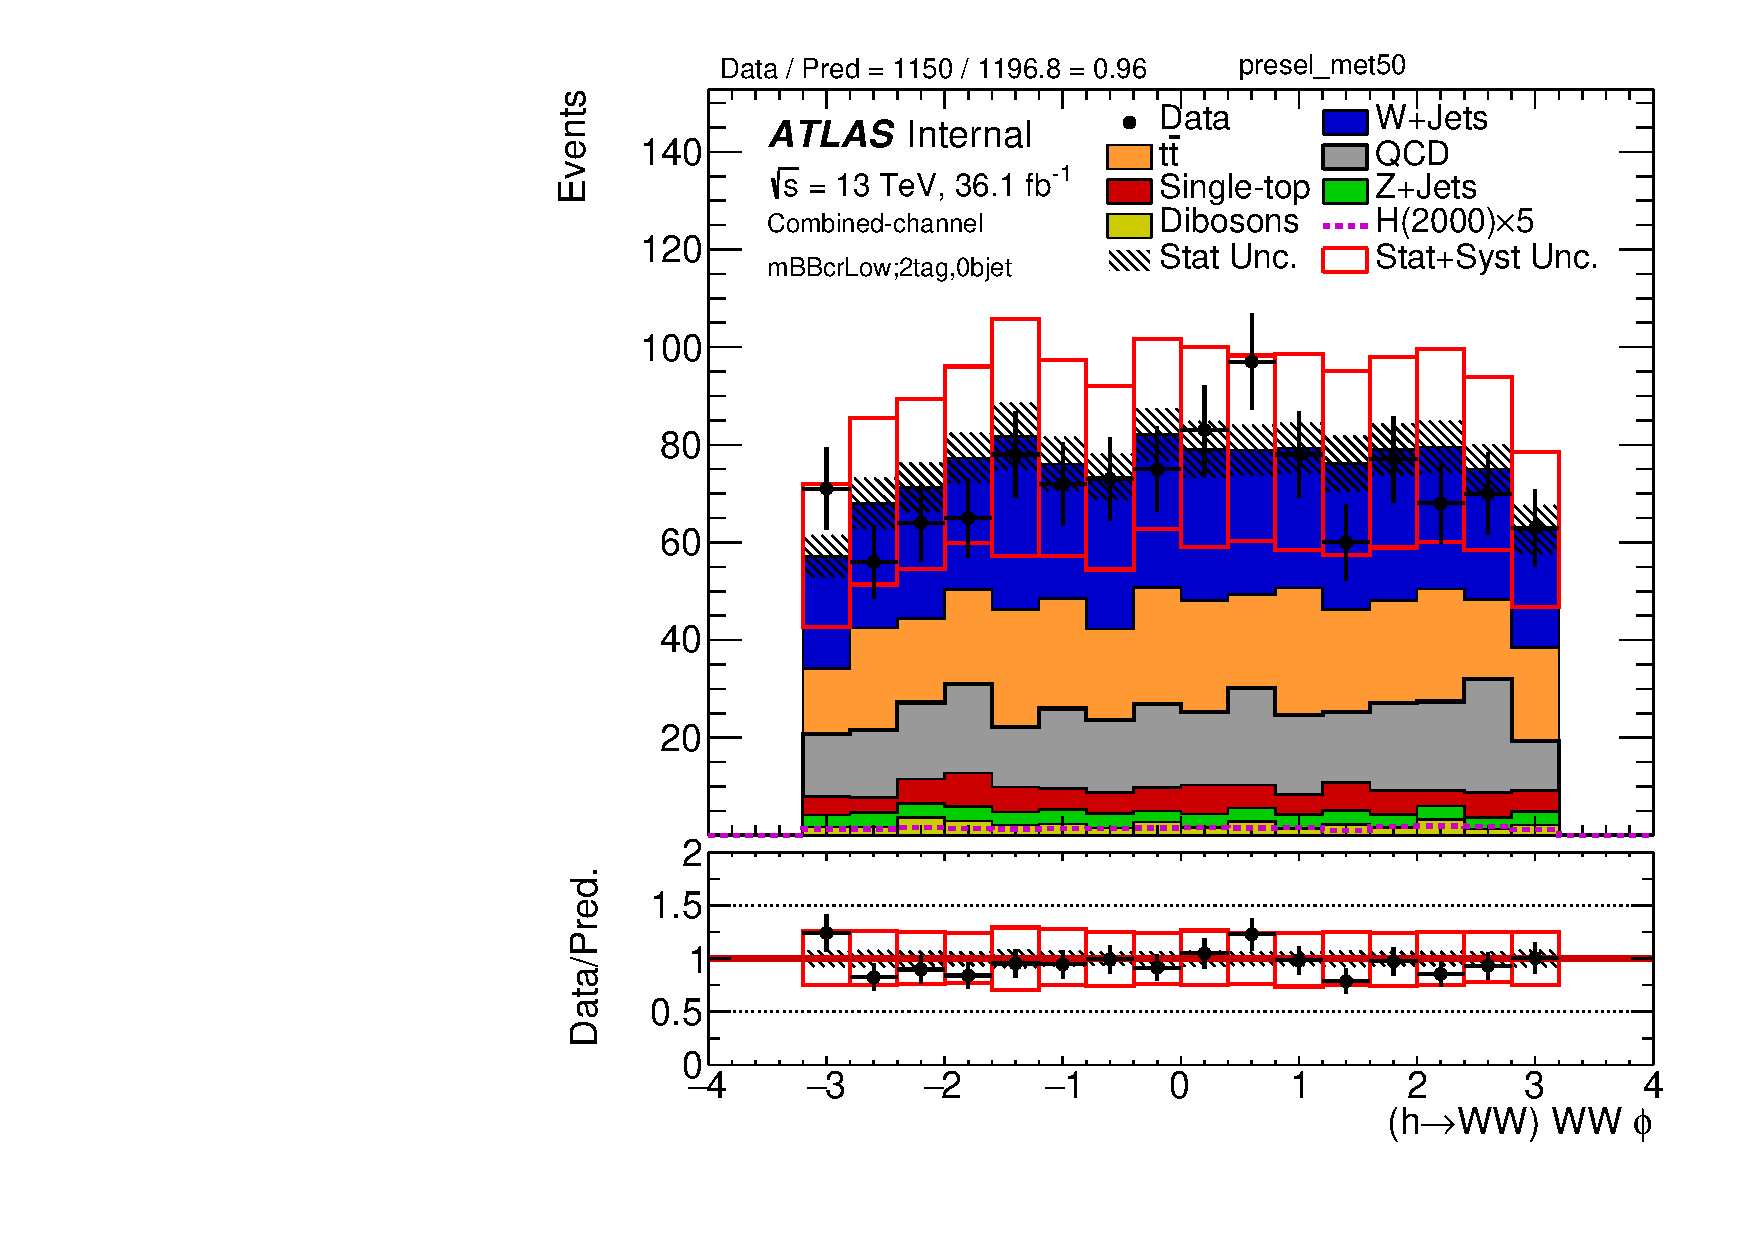
\includegraphics[scale=0.33]{./figures/boosted/PlotByMbbRegions/DataMC_2tag_0bjet_mbbcrLow_lepton_presel_met50_WWPhi}                                                                               
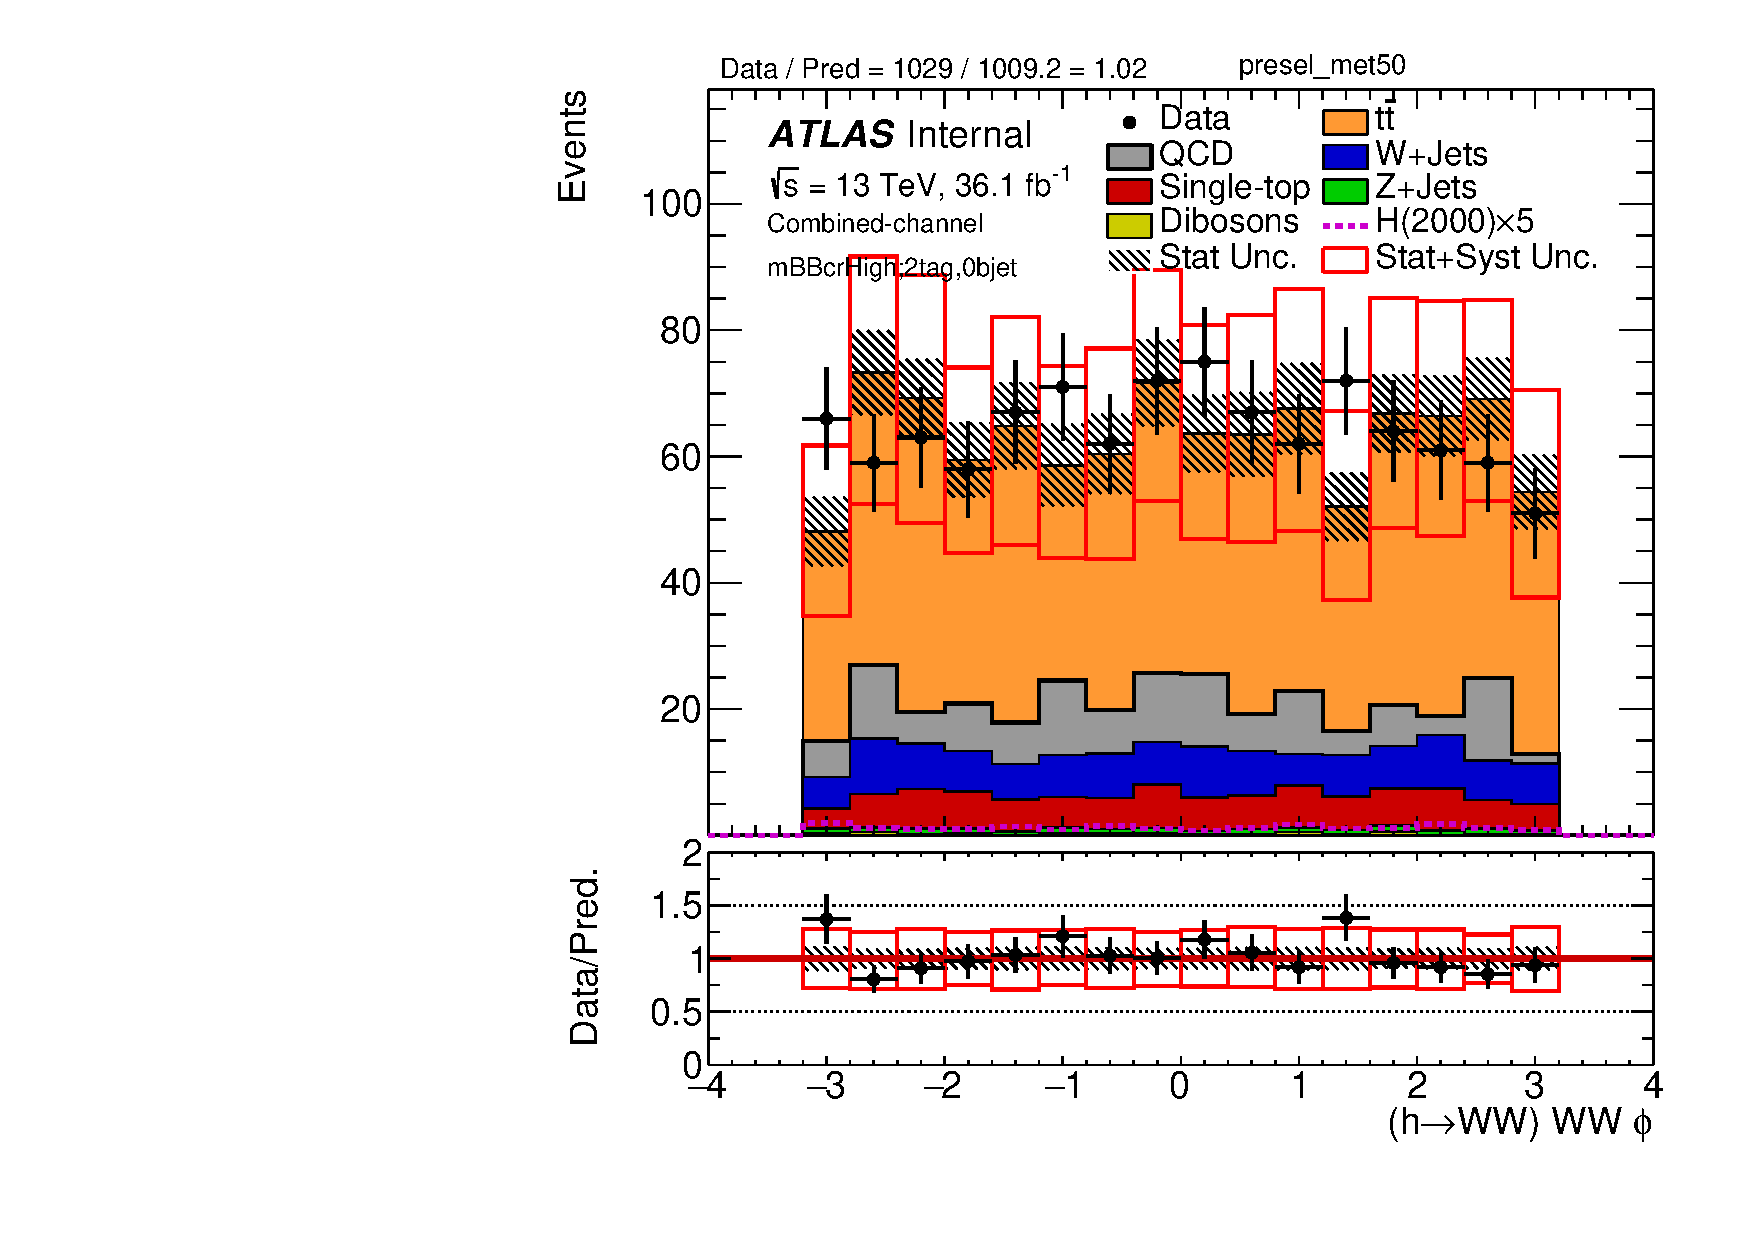
\includegraphics[scale=0.33]{./figures/boosted/PlotByMbbRegions/DataMC_2tag_0bjet_mbbcrHigh_lepton_presel_met50_WWPhi}                                                                              
\caption{Kinematic distributions of the reconstructed $h \to WW$ system in the low (left) and high (right) mBB control region.}
\label{fig:boosted_mbbcrHighLow_wwsystem}
\end{center}
\end{figure}

\begin{figure}[!h]
\begin{center}
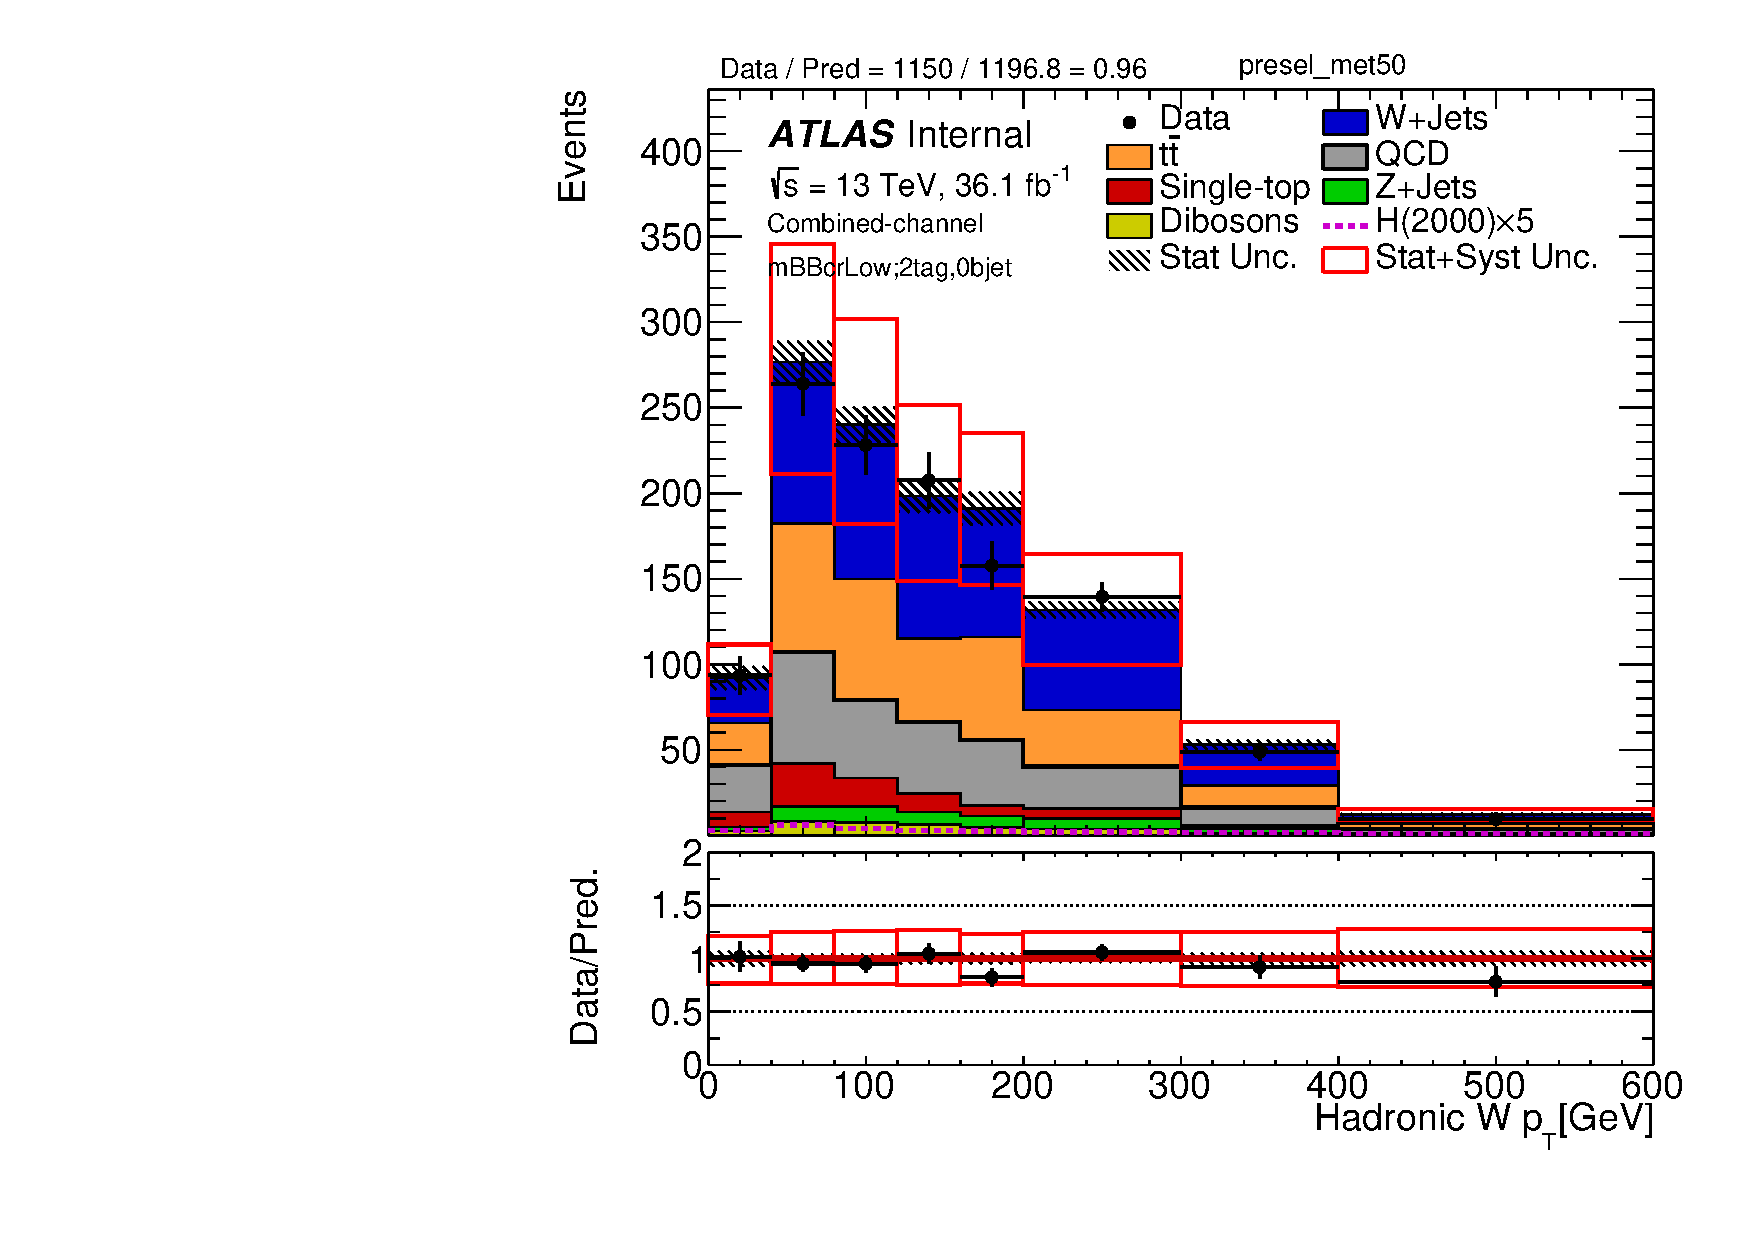
\includegraphics[scale=0.33]{./figures/boosted/PlotByMbbRegions/DataMC_2tag_0bjet_mbbcrLow_lepton_presel_met50_WhadPt}                                                                              
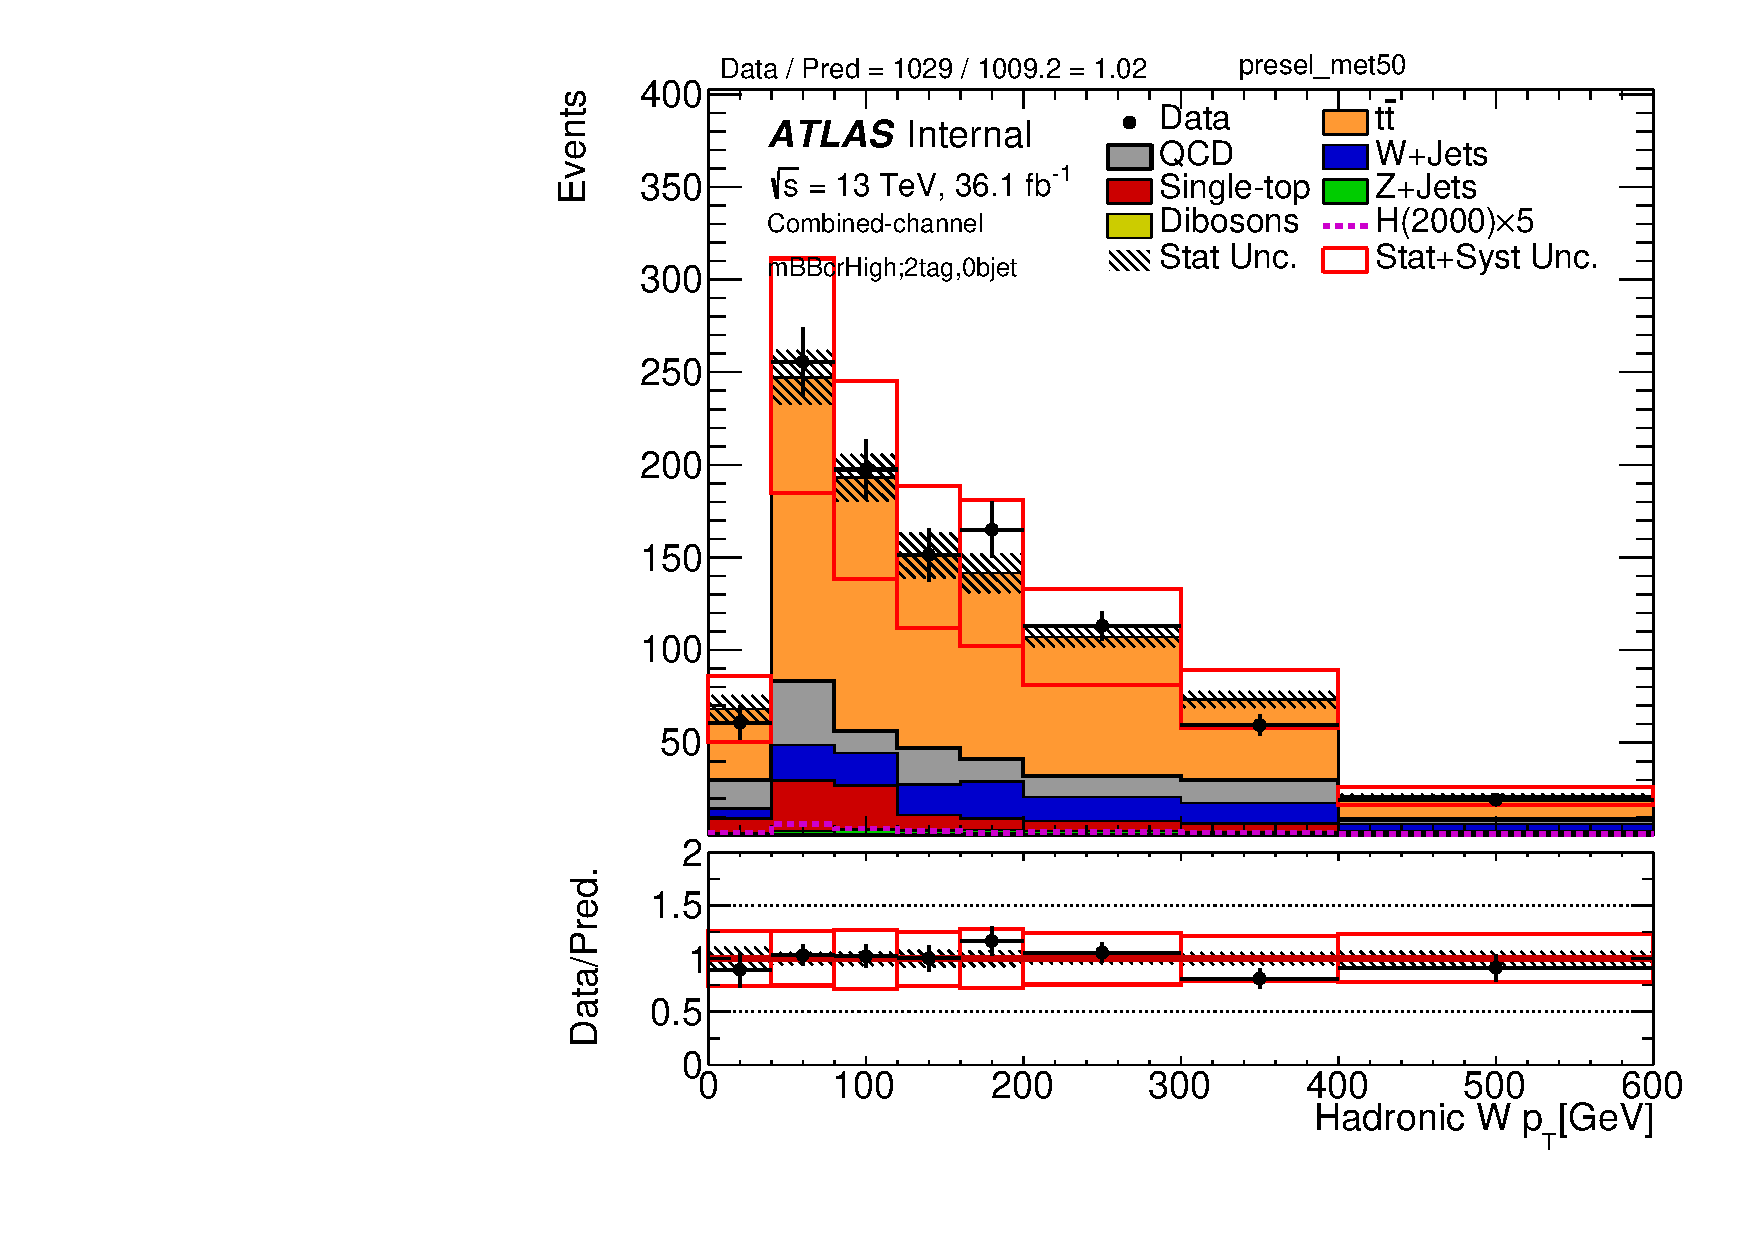
\includegraphics[scale=0.33]{./figures/boosted/PlotByMbbRegions/DataMC_2tag_0bjet_mbbcrHigh_lepton_presel_met50_WhadPt}                                                                             
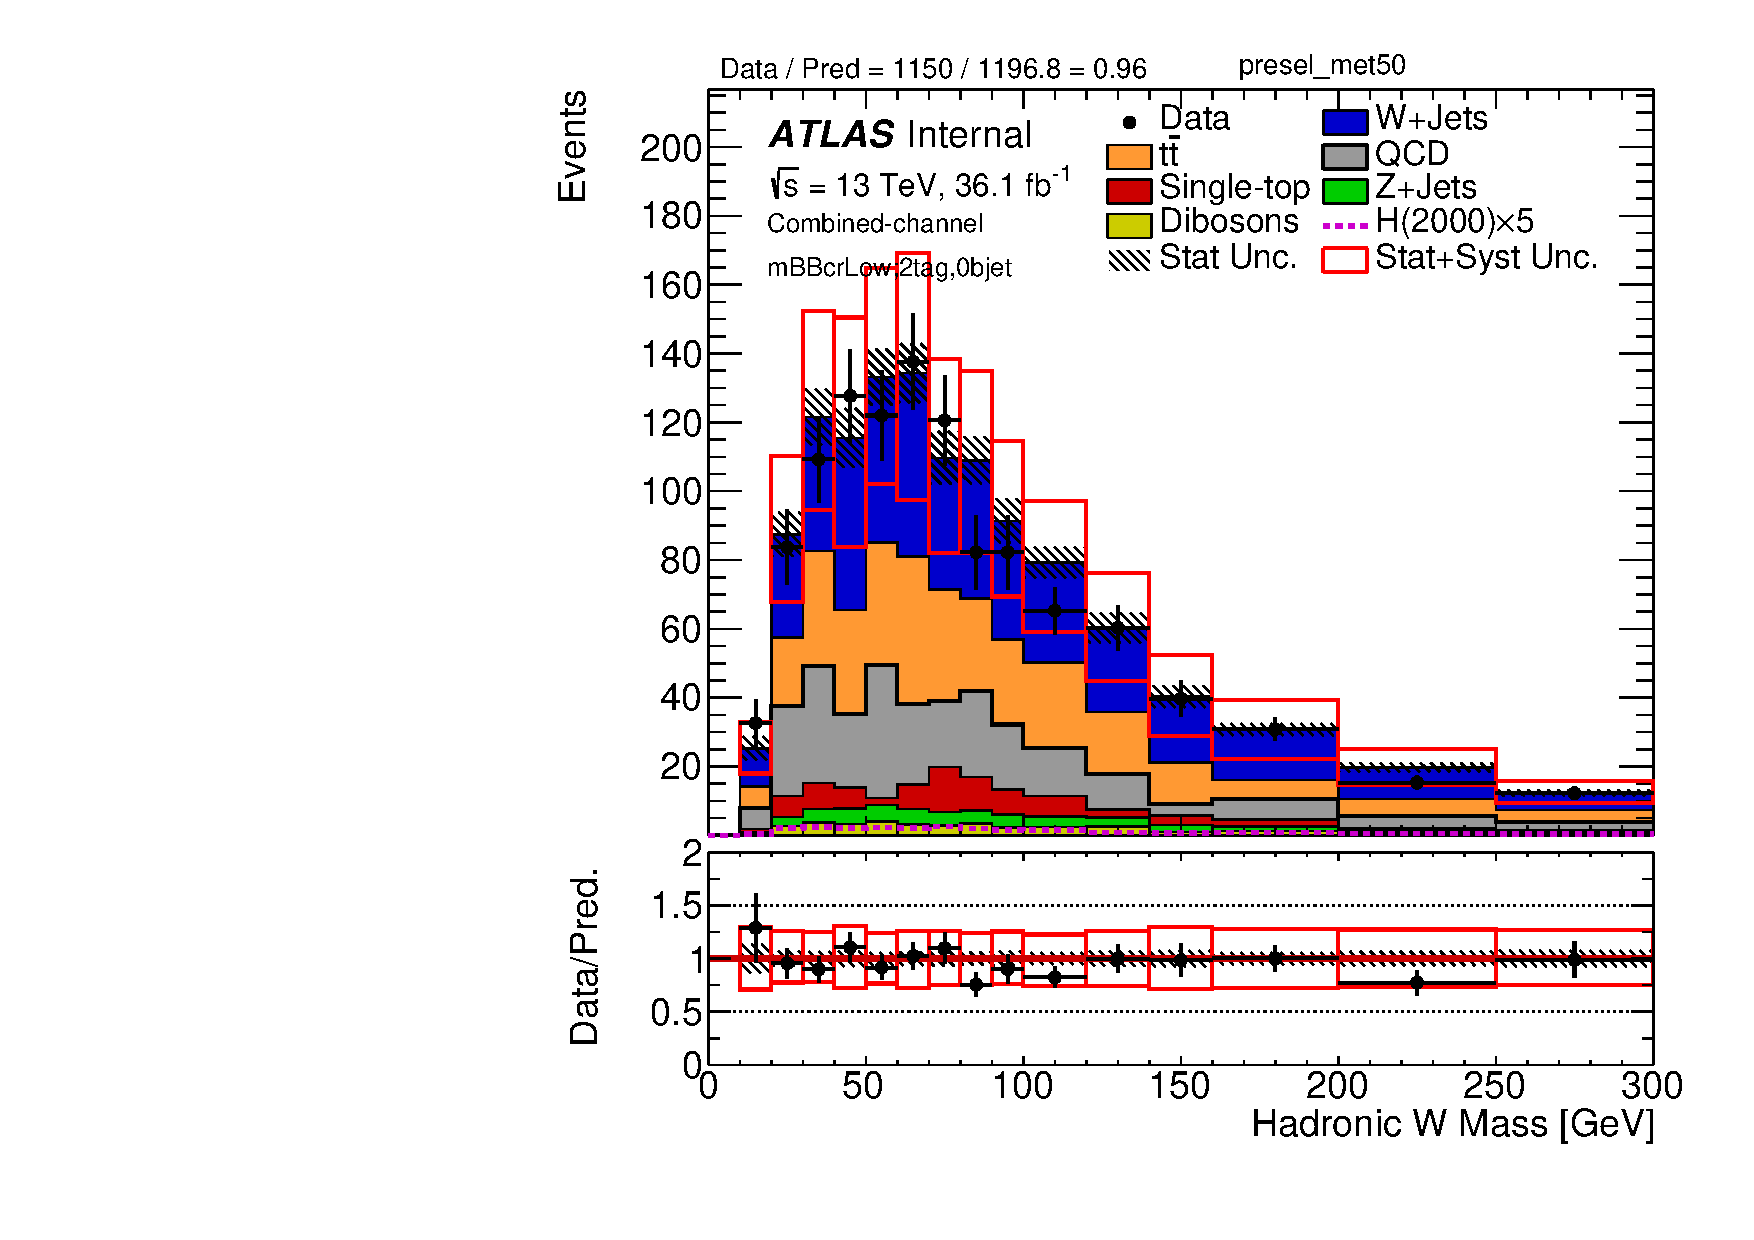
\includegraphics[scale=0.33]{./figures/boosted/PlotByMbbRegions/DataMC_2tag_0bjet_mbbcrLow_lepton_presel_met50_WhadMass}                                                                            
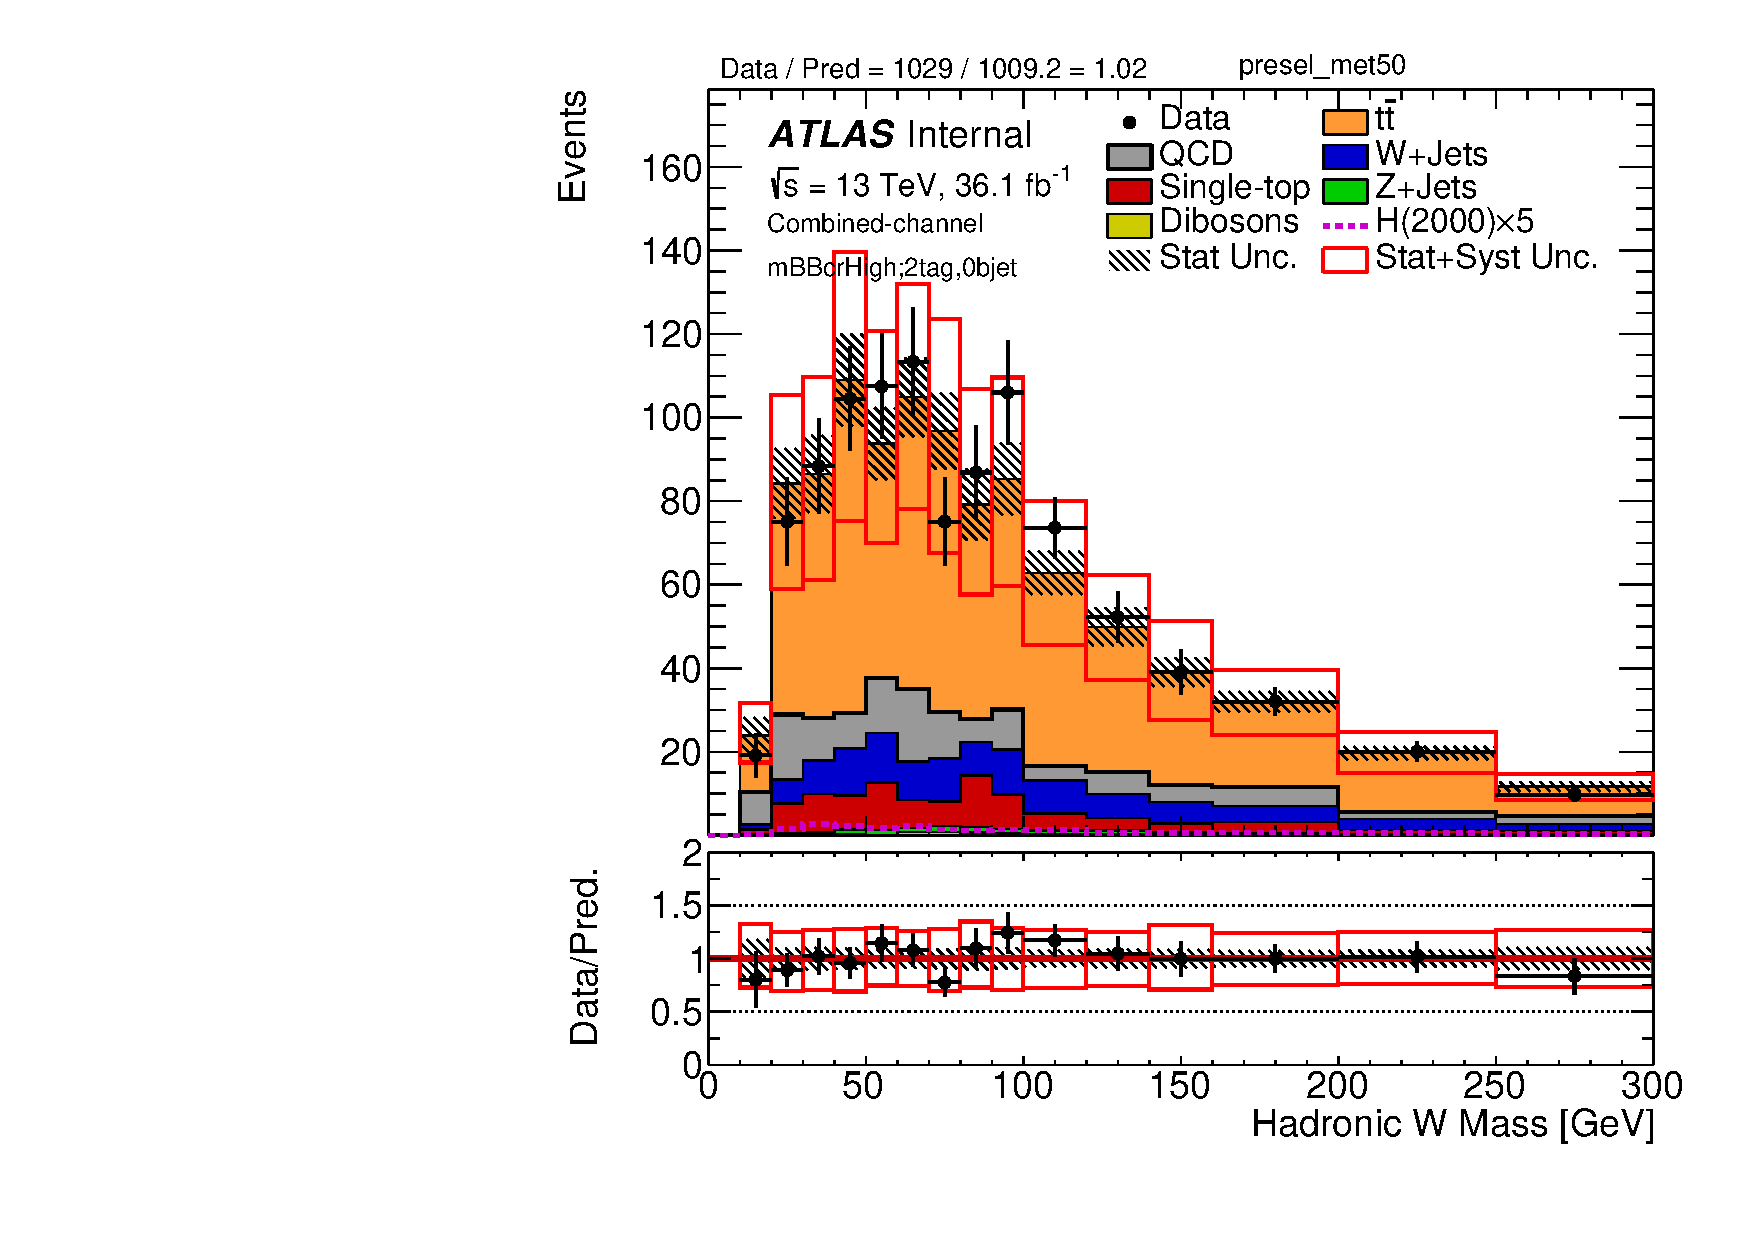
\includegraphics[scale=0.33]{./figures/boosted/PlotByMbbRegions/DataMC_2tag_0bjet_mbbcrHigh_lepton_presel_met50_WhadMass}                                                                           
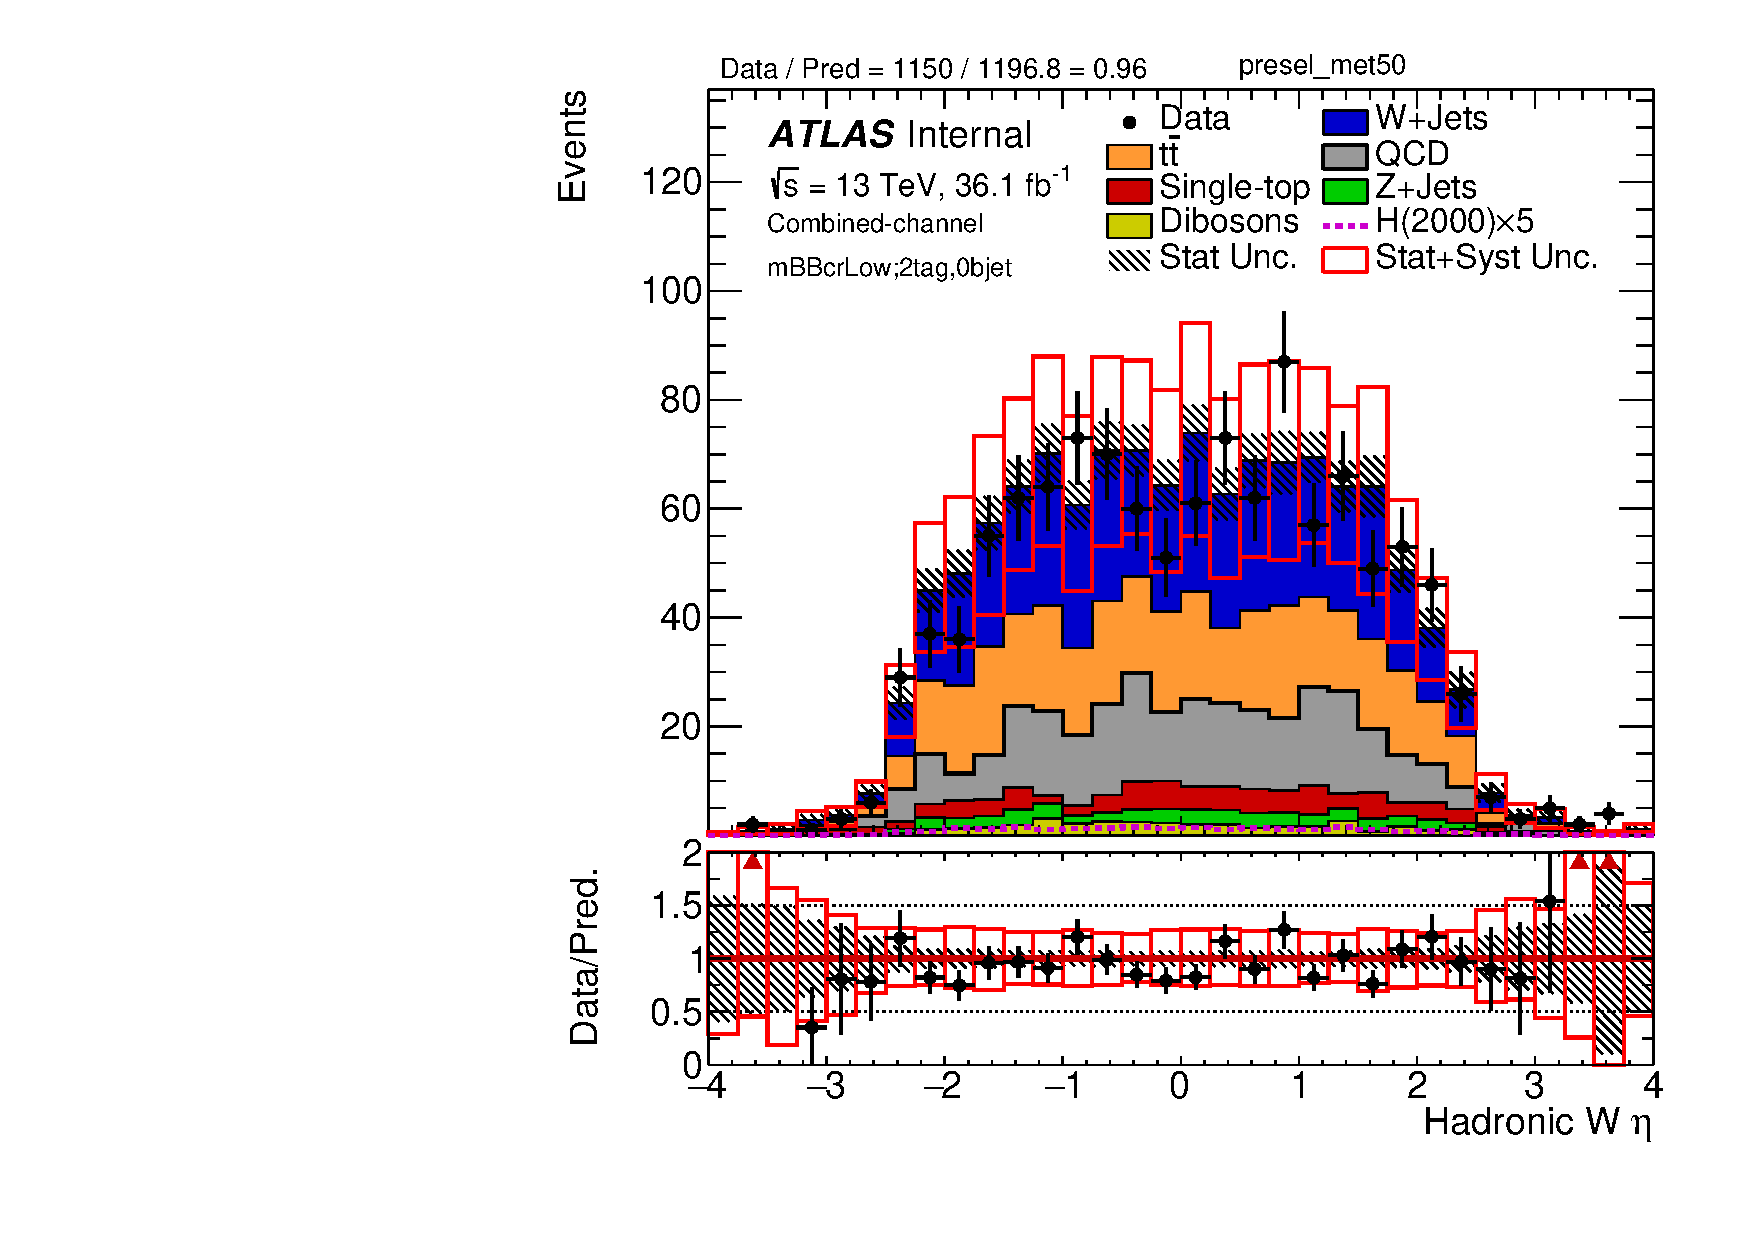
\includegraphics[scale=0.33]{./figures/boosted/PlotByMbbRegions/DataMC_2tag_0bjet_mbbcrLow_lepton_presel_met50_WhadEta}                                                                             
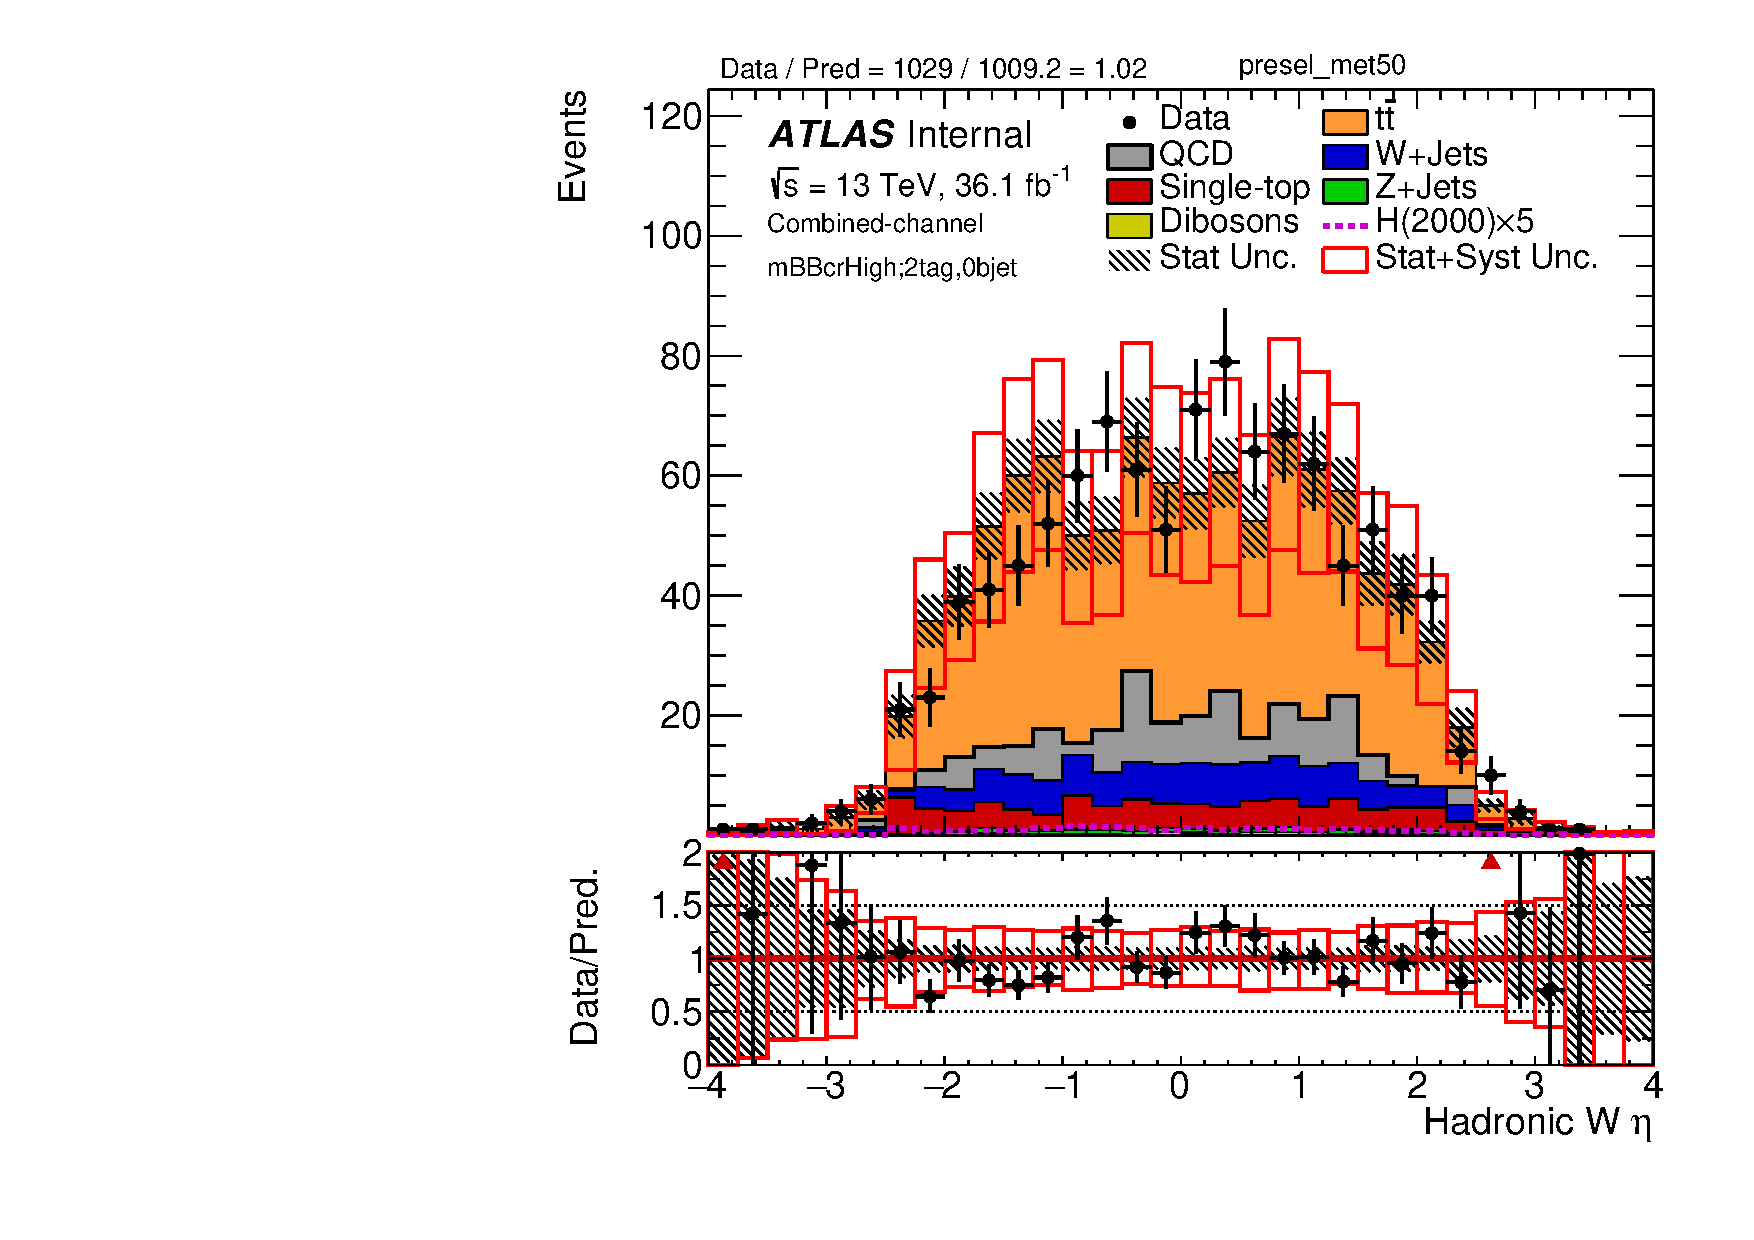
\includegraphics[scale=0.33]{./figures/boosted/PlotByMbbRegions/DataMC_2tag_0bjet_mbbcrHigh_lepton_presel_met50_WhadEta}                                                                            
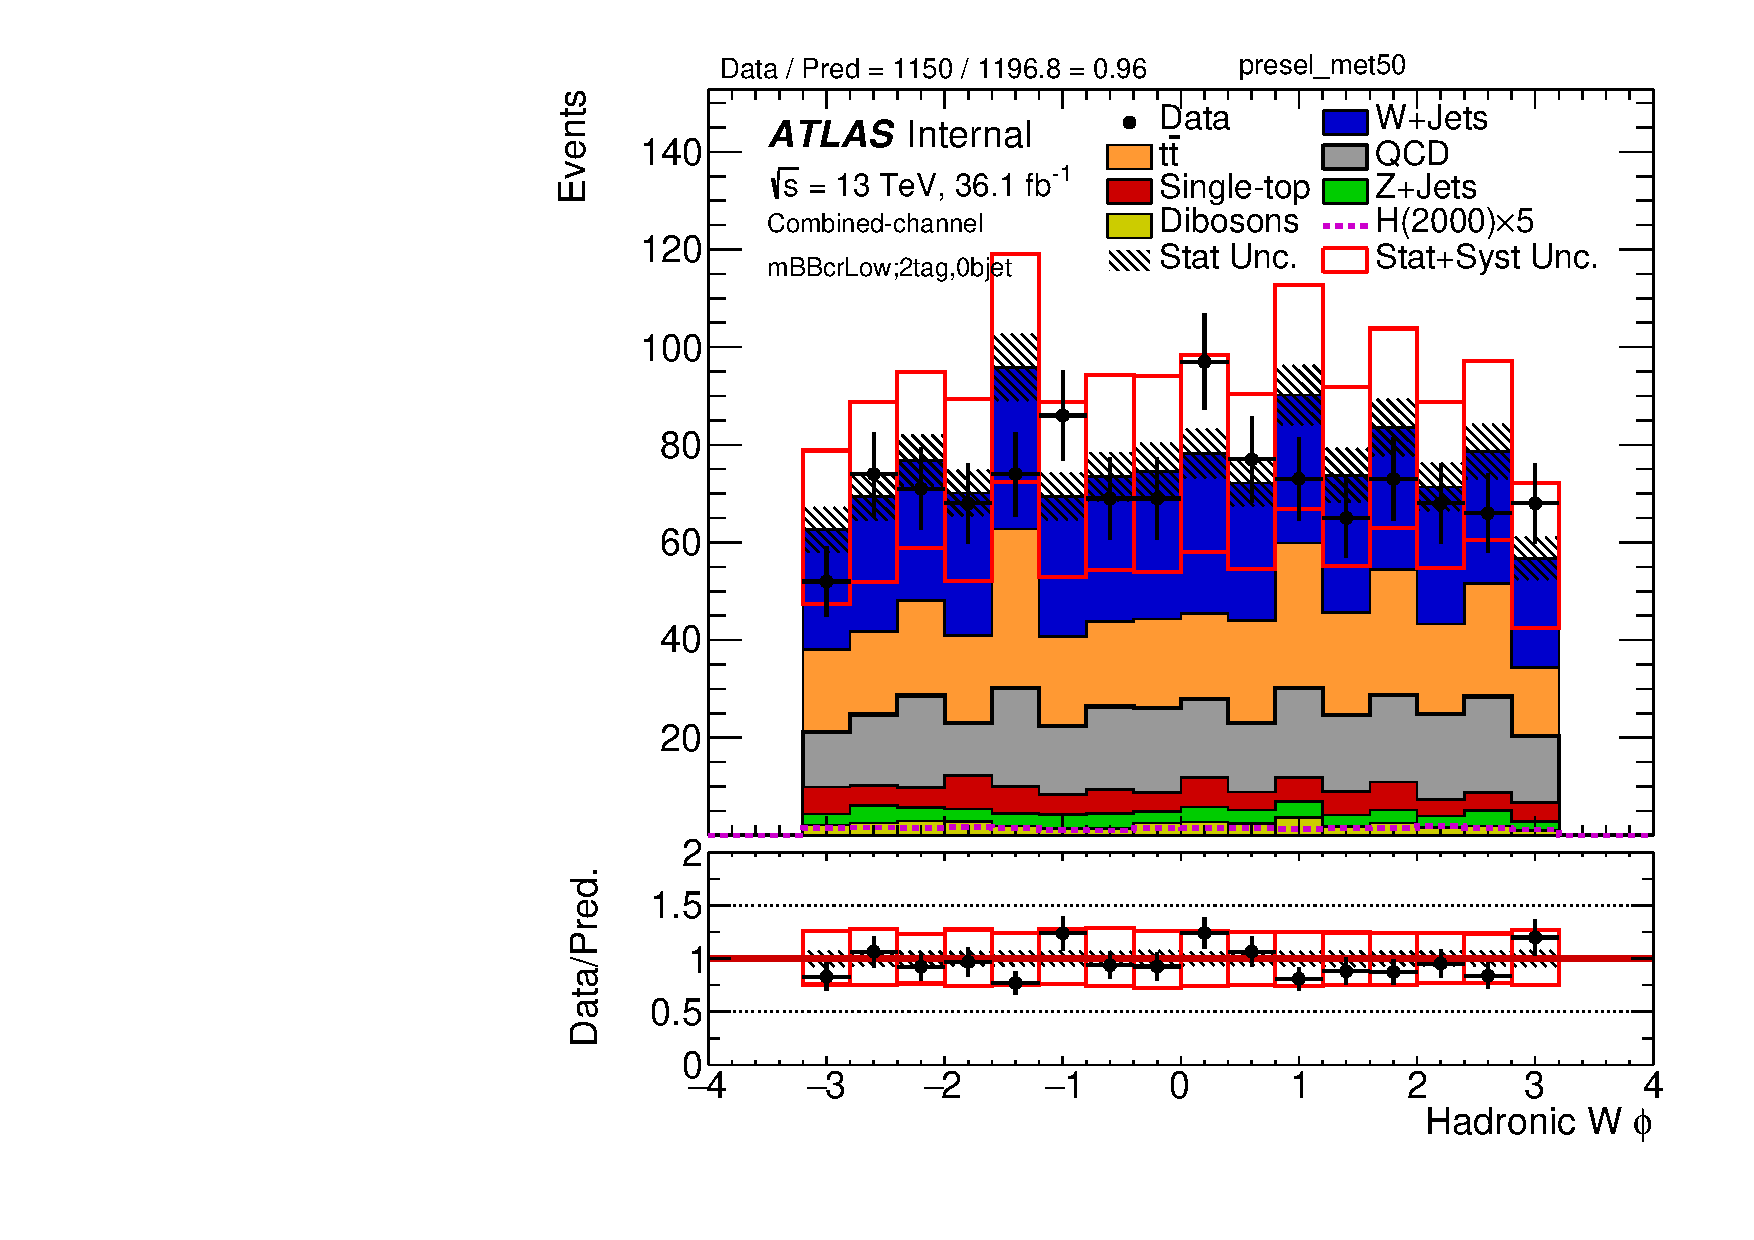
\includegraphics[scale=0.33]{./figures/boosted/PlotByMbbRegions/DataMC_2tag_0bjet_mbbcrLow_lepton_presel_met50_WhadPhi}                                                                             
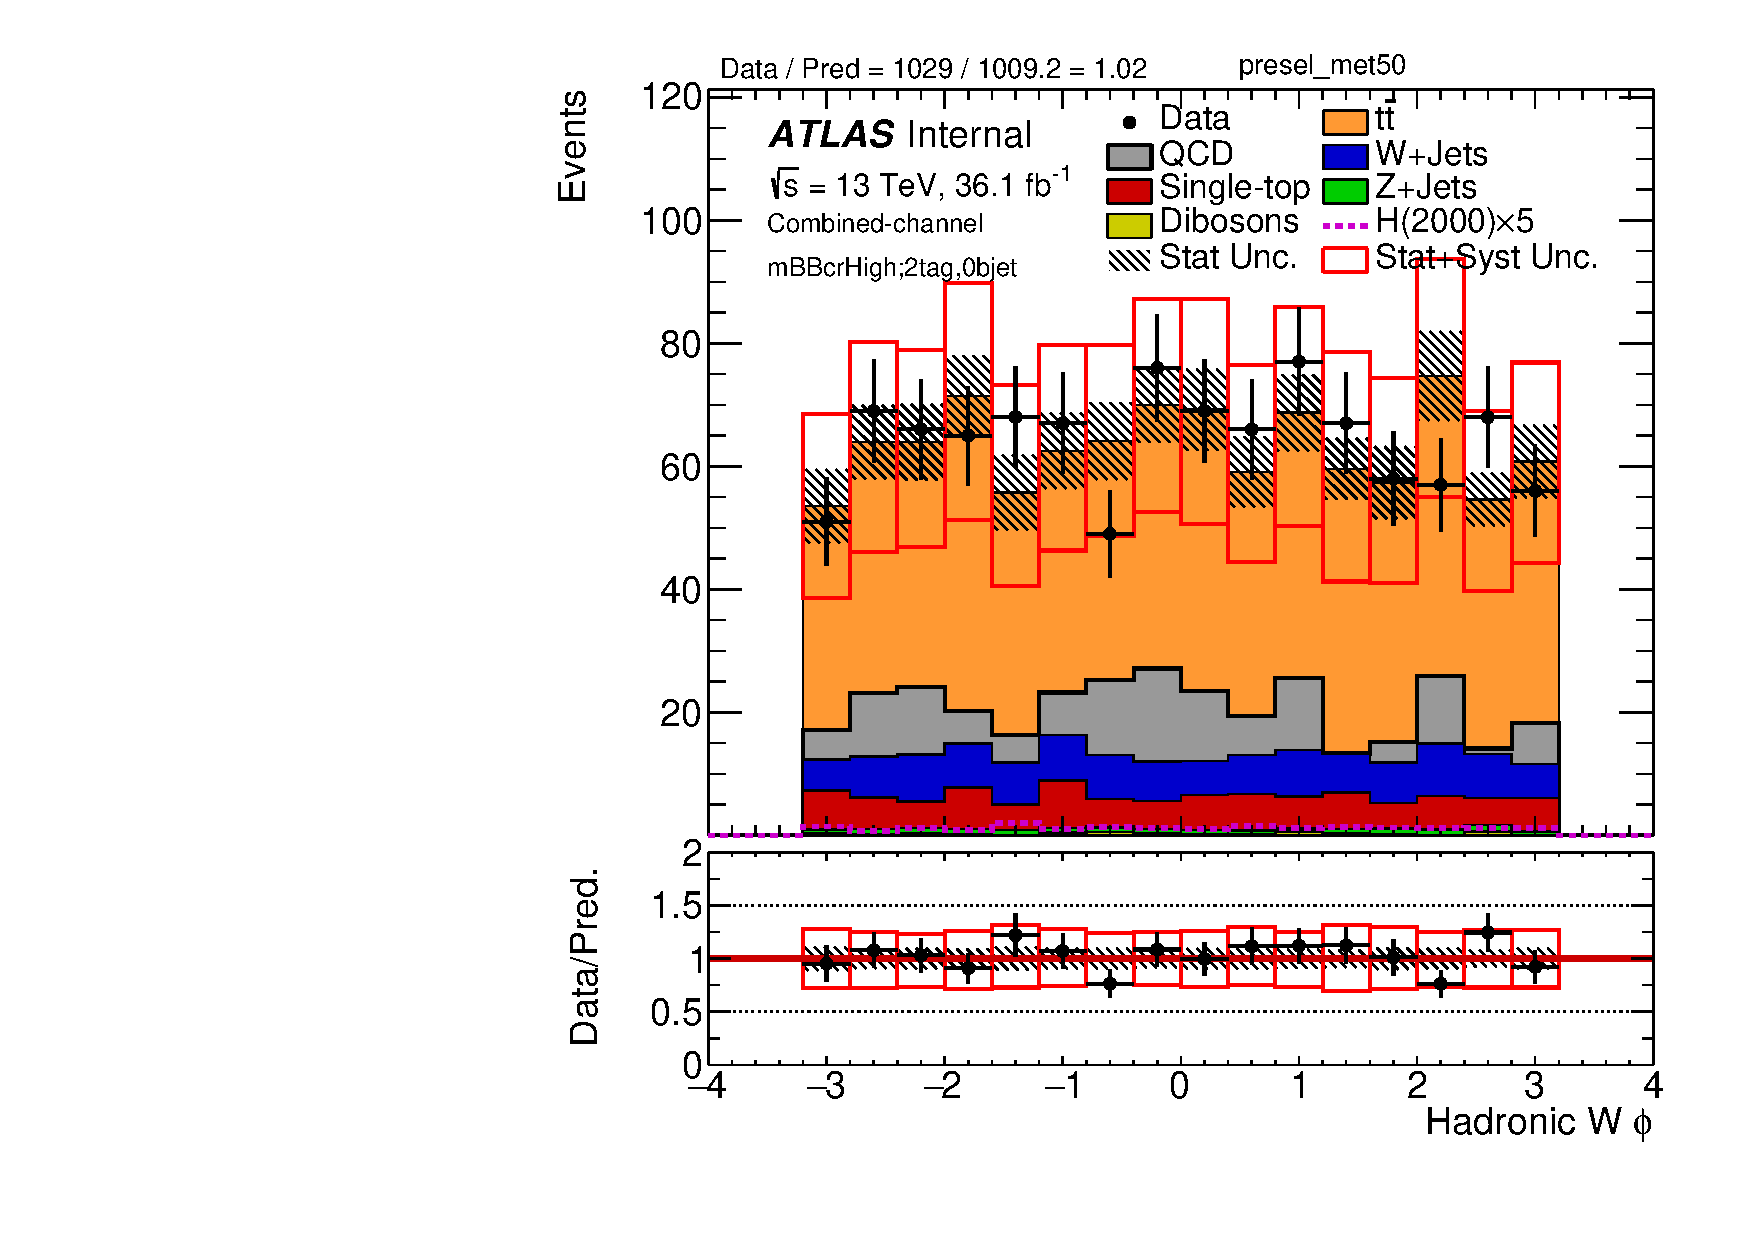
\includegraphics[scale=0.33]{./figures/boosted/PlotByMbbRegions/DataMC_2tag_0bjet_mbbcrHigh_lepton_presel_met50_WhadPhi}                                                                            
\caption{Kinematic distributions of the reconstructed $W \to q\bar{q}$ system in the low (left) and high (right) mBB control region.}
\label{fig:boosted_mbbcrHighLow_whad}
\end{center}
\end{figure}

\begin{figure}[!h]
\begin{center}
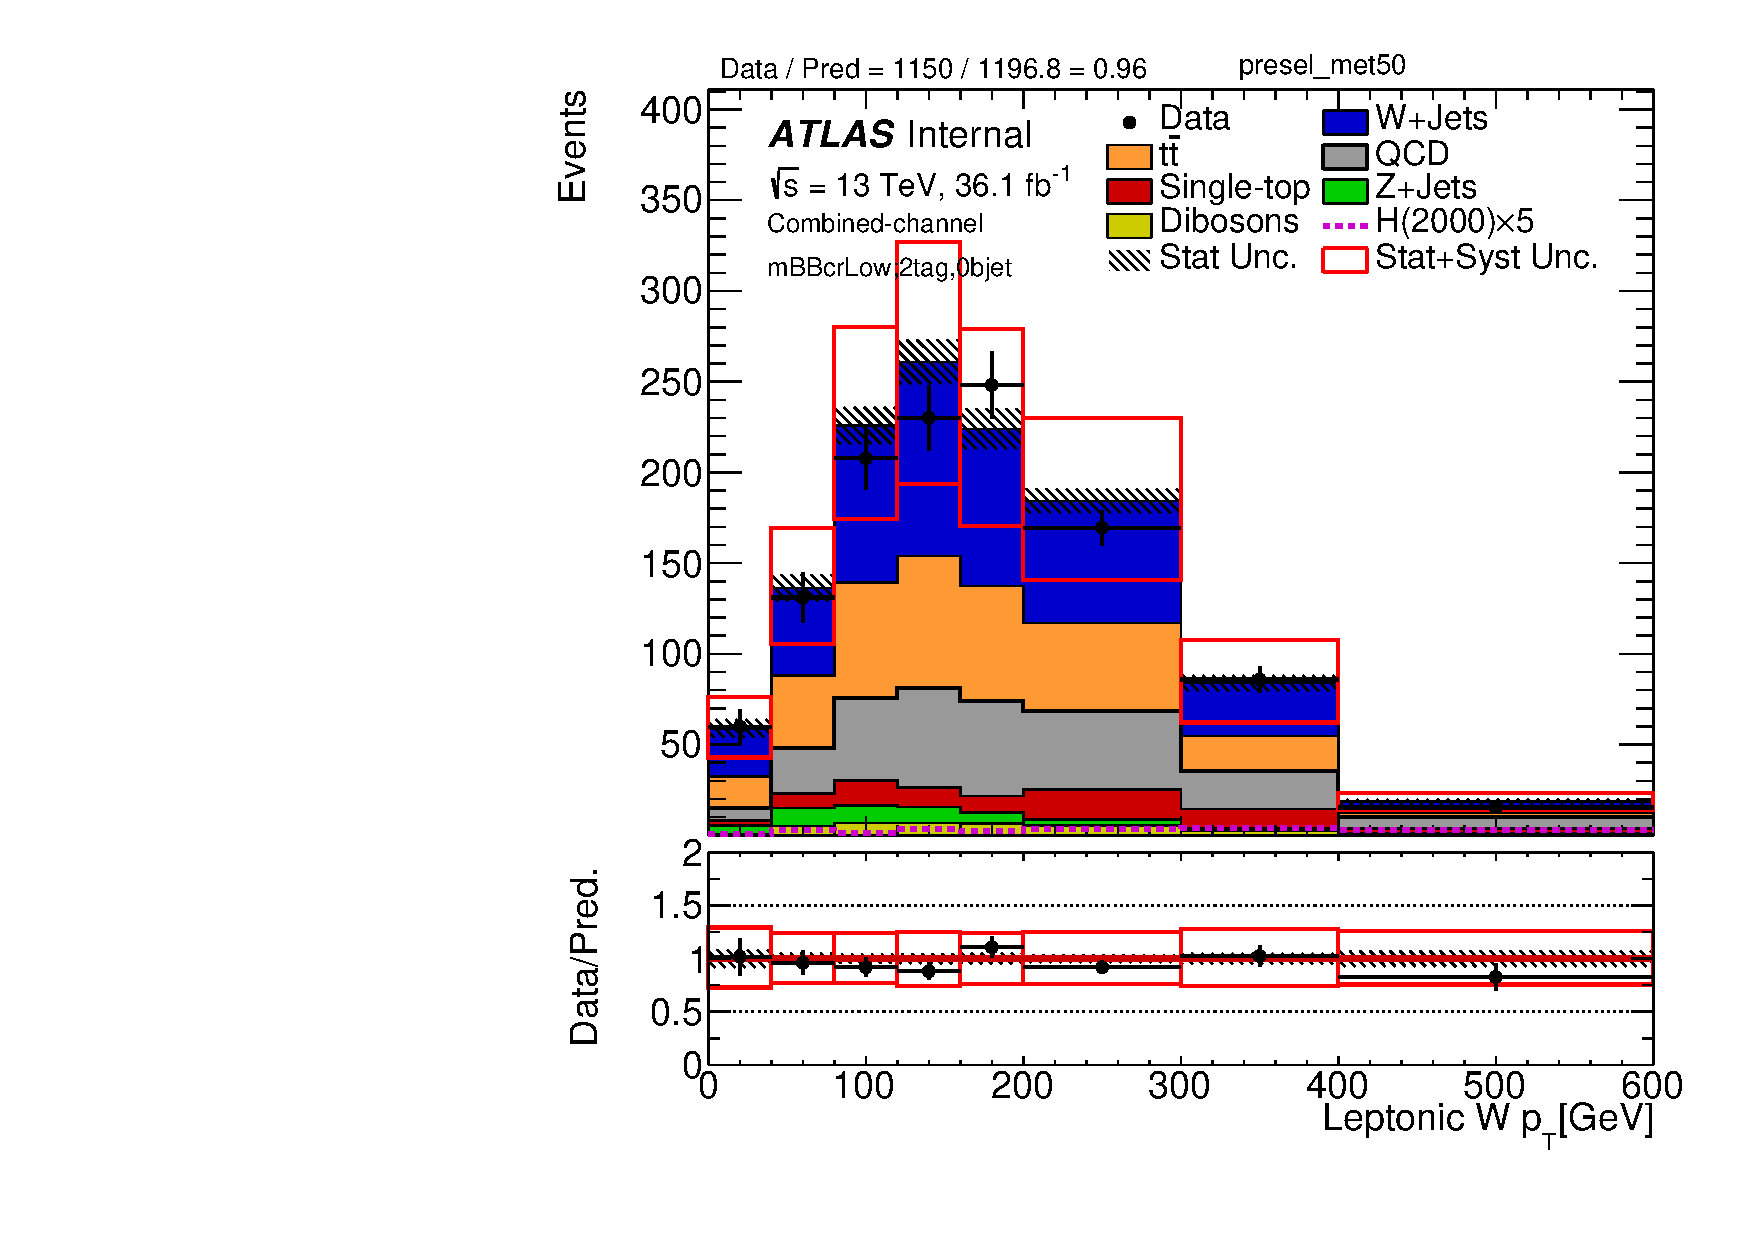
\includegraphics[scale=0.33]{./figures/boosted/PlotByMbbRegions/DataMC_2tag_0bjet_mbbcrLow_lepton_presel_met50_WlepPt}                                                                              
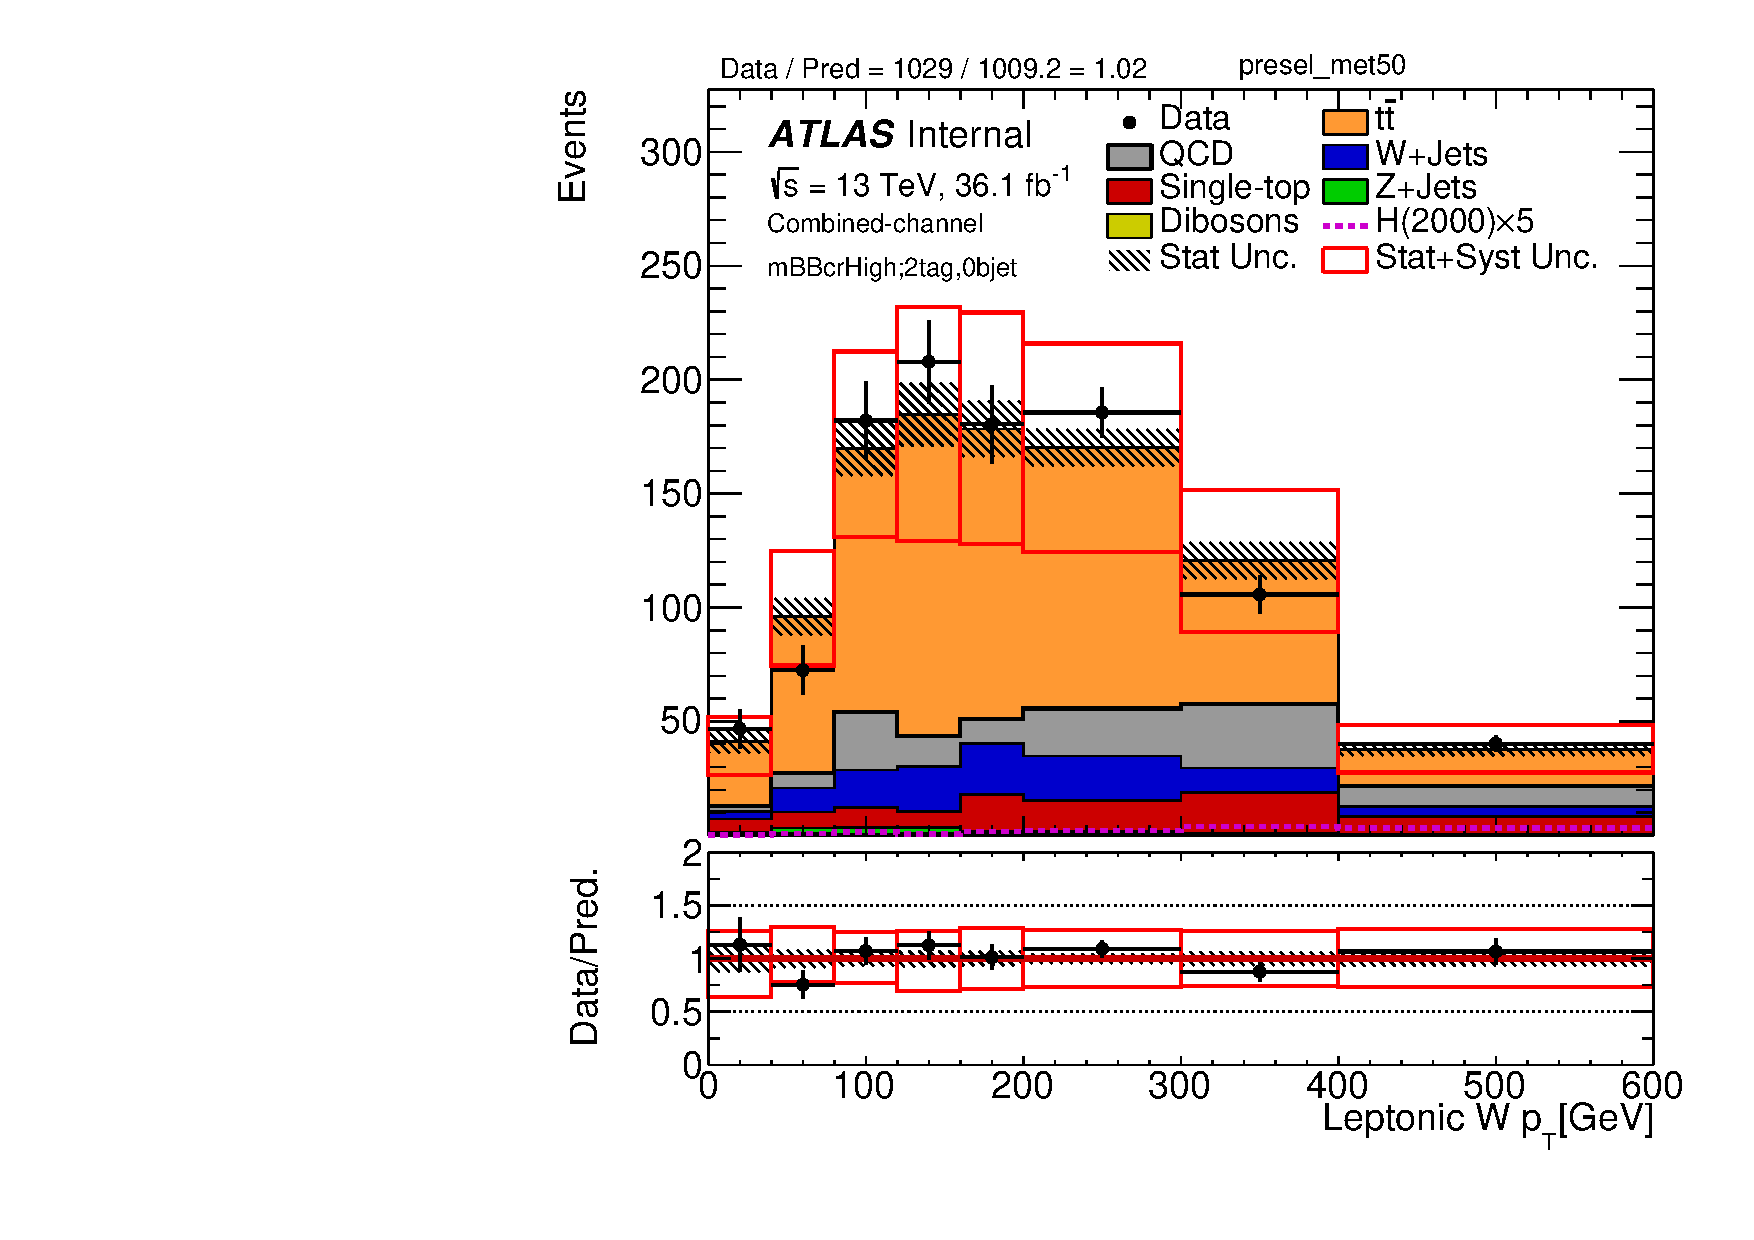
\includegraphics[scale=0.33]{./figures/boosted/PlotByMbbRegions/DataMC_2tag_0bjet_mbbcrHigh_lepton_presel_met50_WlepPt}                                                                             
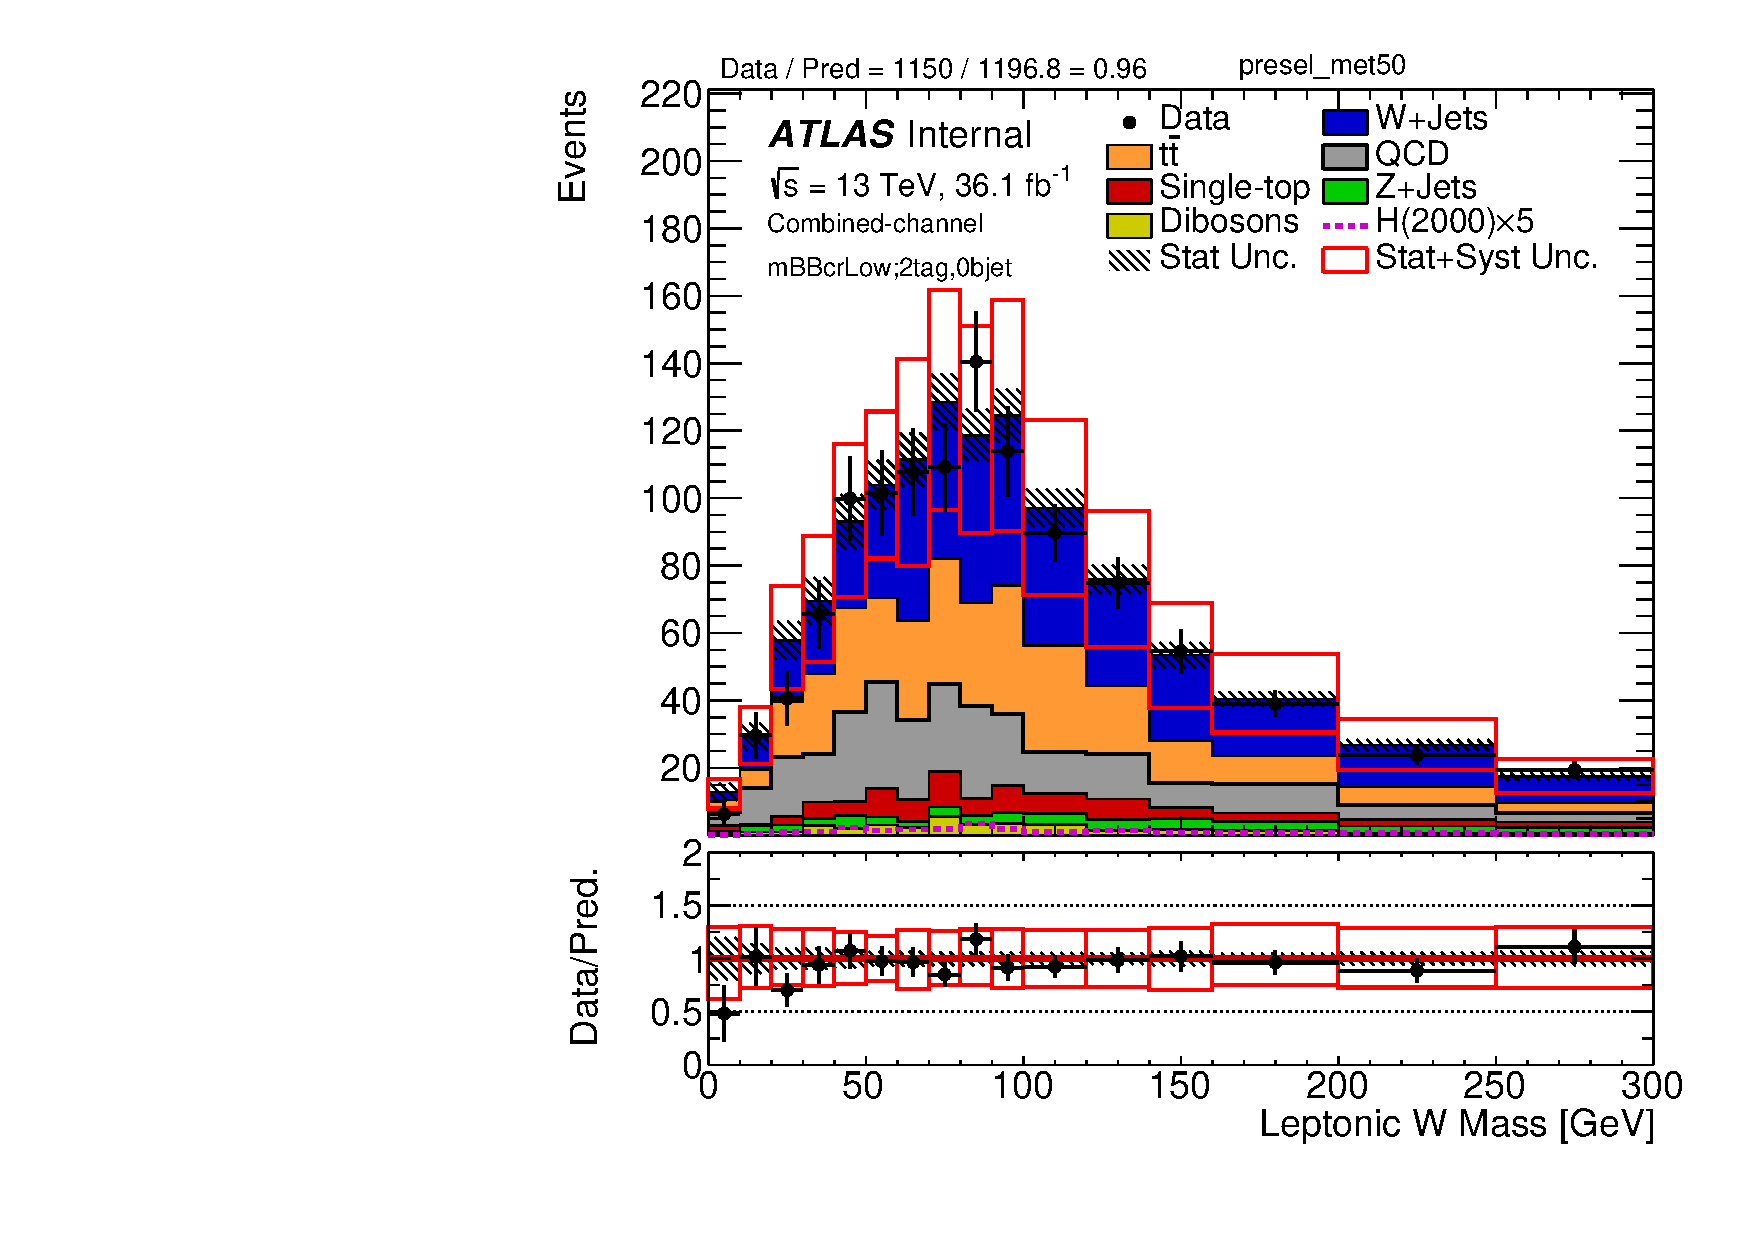
\includegraphics[scale=0.33]{./figures/boosted/PlotByMbbRegions/DataMC_2tag_0bjet_mbbcrLow_lepton_presel_met50_WlepMass}                                                                            
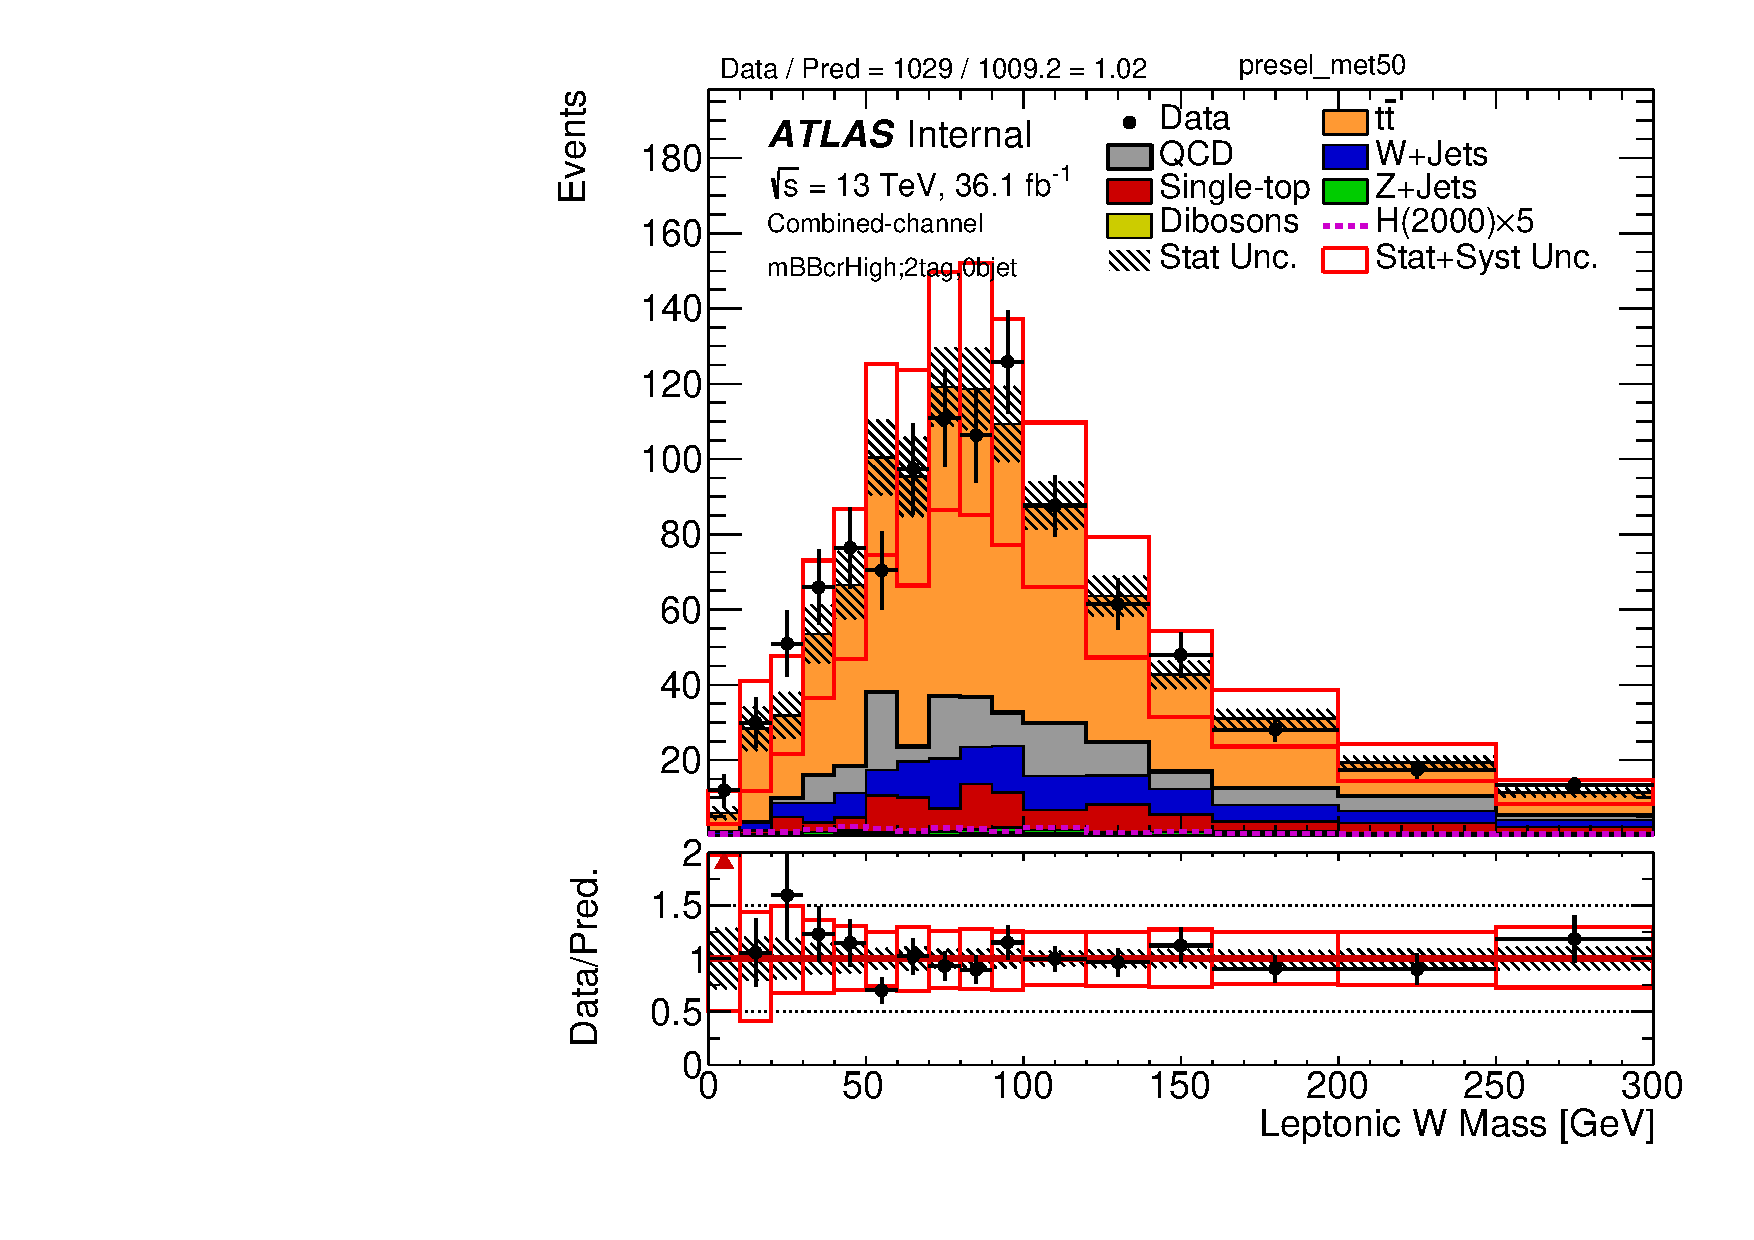
\includegraphics[scale=0.33]{./figures/boosted/PlotByMbbRegions/DataMC_2tag_0bjet_mbbcrHigh_lepton_presel_met50_WlepMass}                                                                           
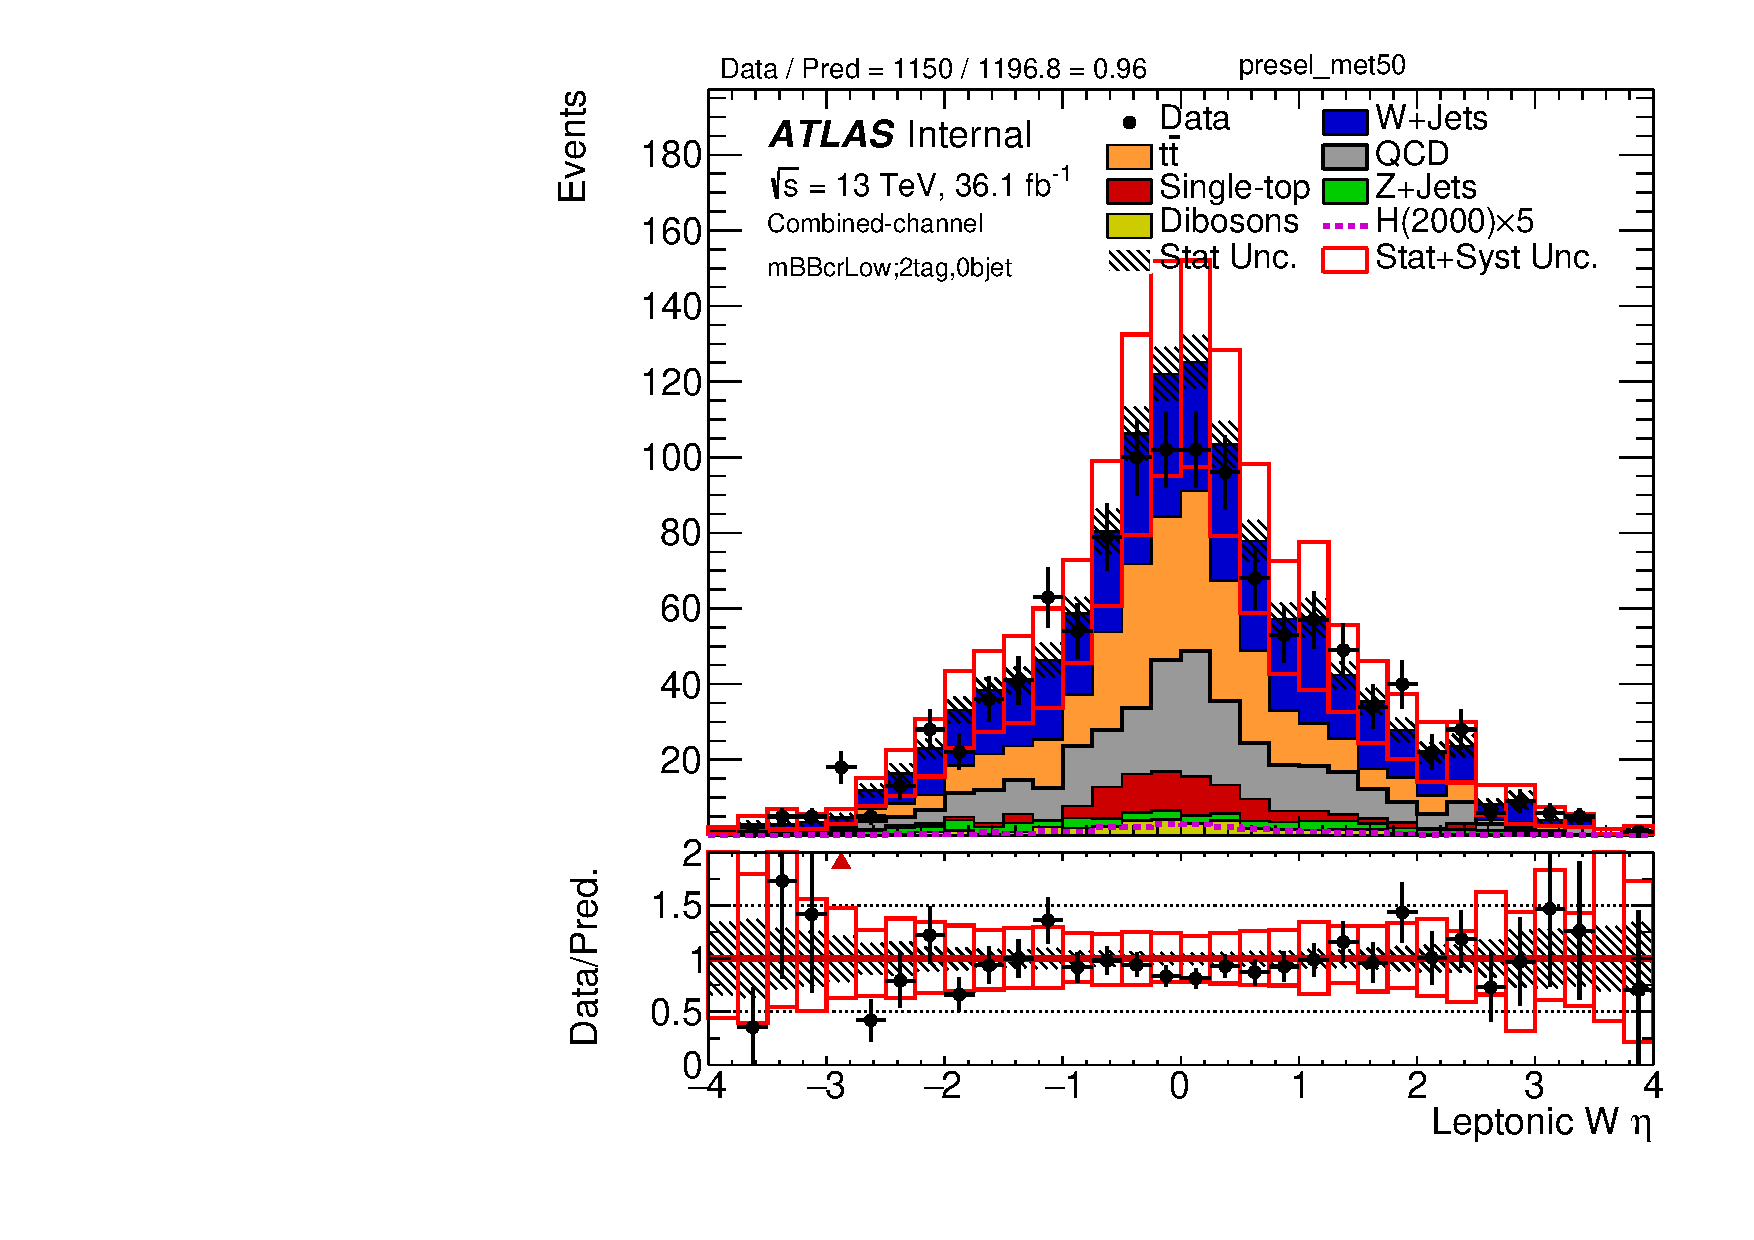
\includegraphics[scale=0.33]{./figures/boosted/PlotByMbbRegions/DataMC_2tag_0bjet_mbbcrLow_lepton_presel_met50_WlepEta}                                                                             
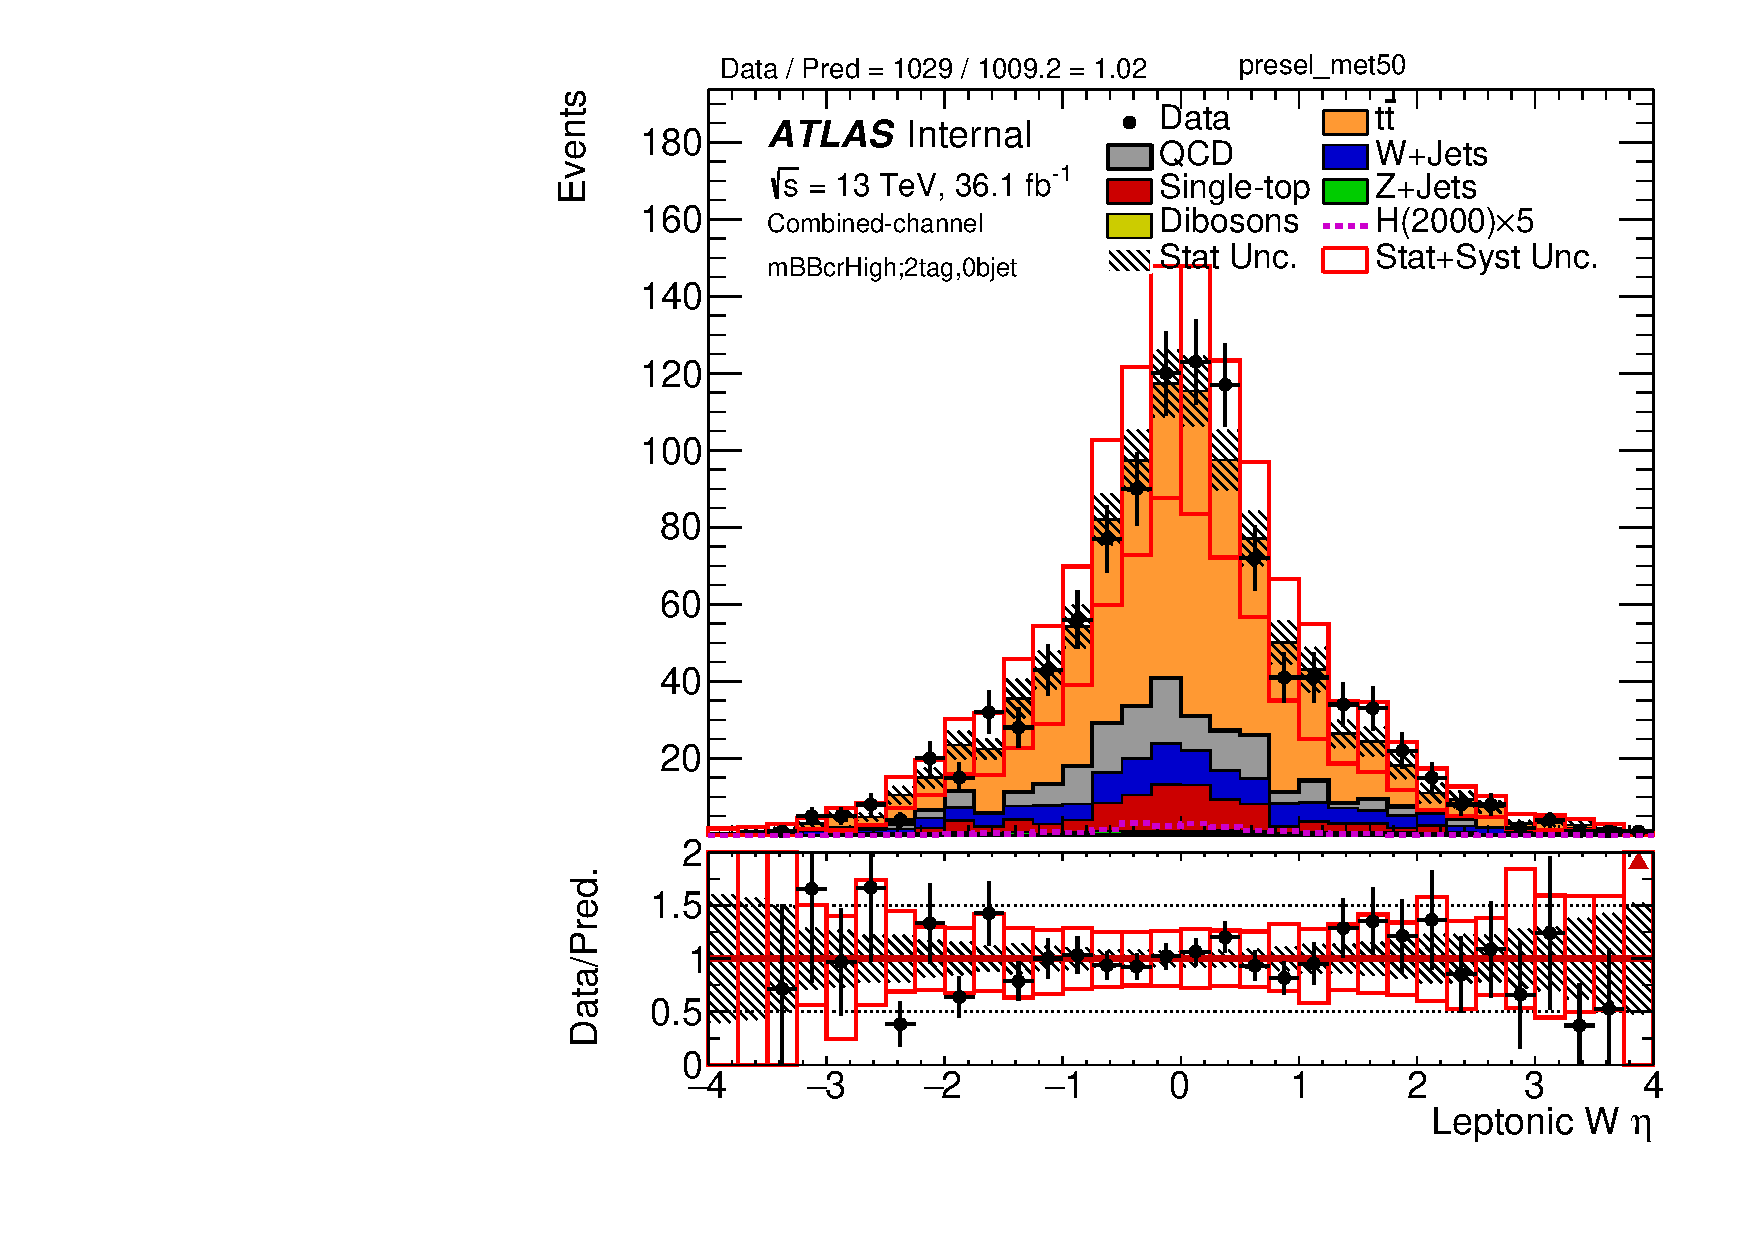
\includegraphics[scale=0.33]{./figures/boosted/PlotByMbbRegions/DataMC_2tag_0bjet_mbbcrHigh_lepton_presel_met50_WlepEta}                                                                            
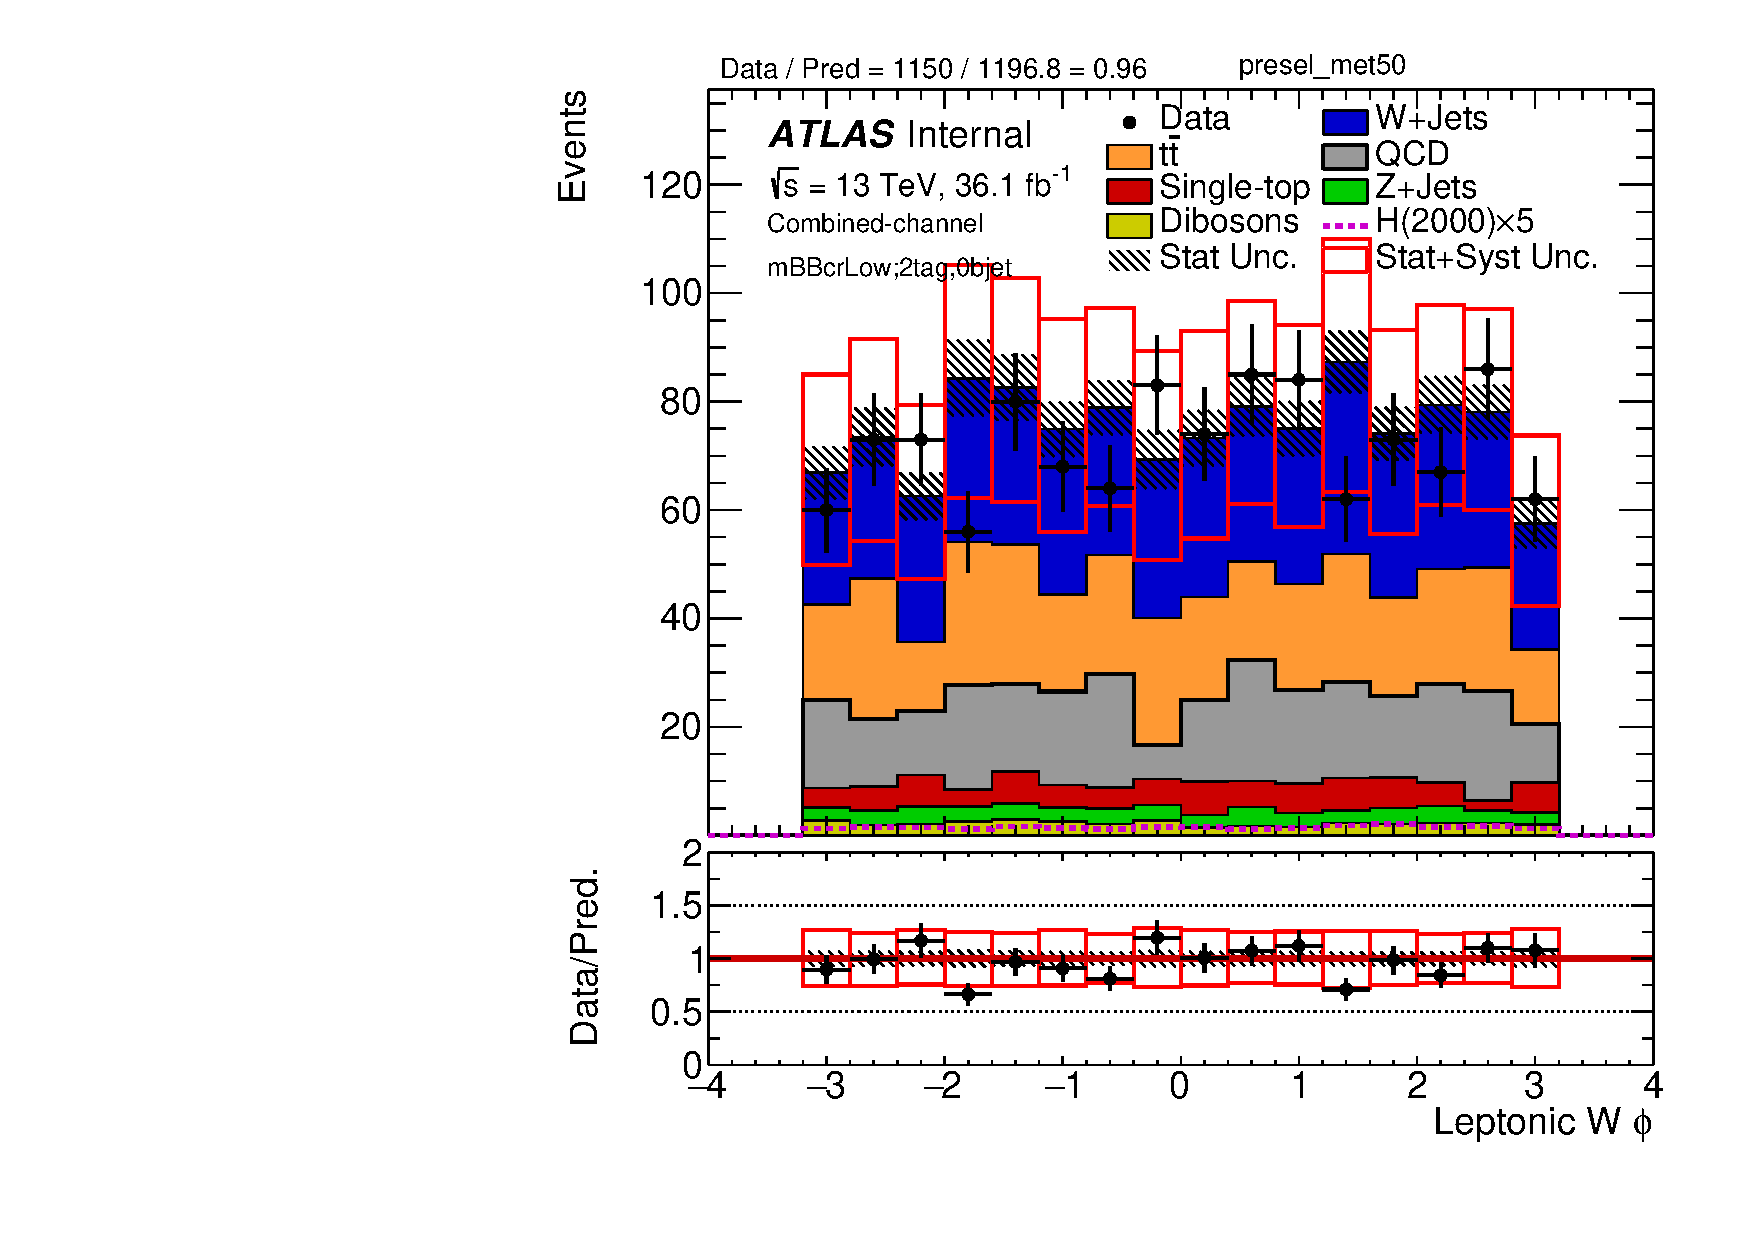
\includegraphics[scale=0.33]{./figures/boosted/PlotByMbbRegions/DataMC_2tag_0bjet_mbbcrLow_lepton_presel_met50_WlepPhi}                                                                             
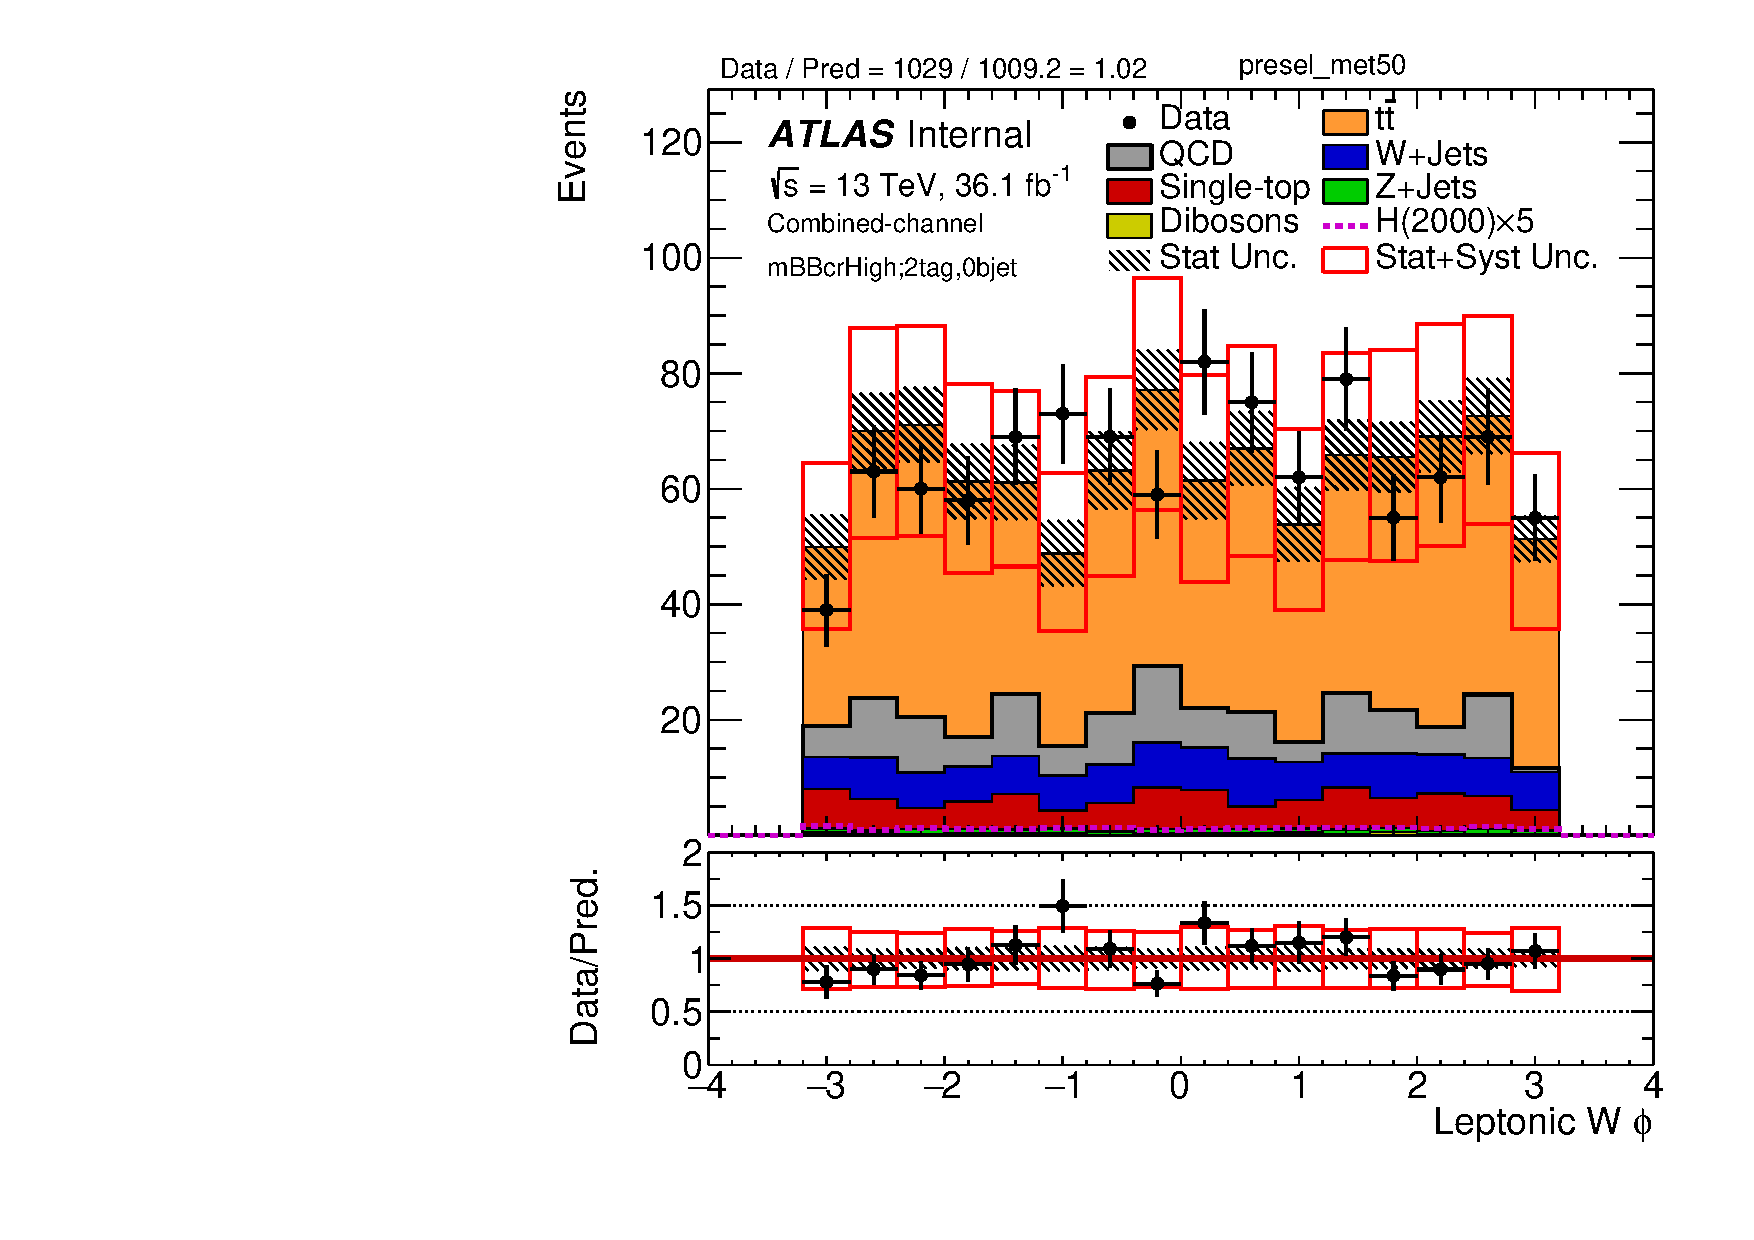
\includegraphics[scale=0.33]{./figures/boosted/PlotByMbbRegions/DataMC_2tag_0bjet_mbbcrHigh_lepton_presel_met50_WlepPhi}                                                                            
\caption{Kinematic distributions of the reconstructed $W \to l\nu$ system in the low (left) and high (right) mBB control region.}
\label{fig:boosted_mbbcrHighLow_wlep}
\end{center}
\end{figure}

\begin{figure}[!h]
\begin{center}
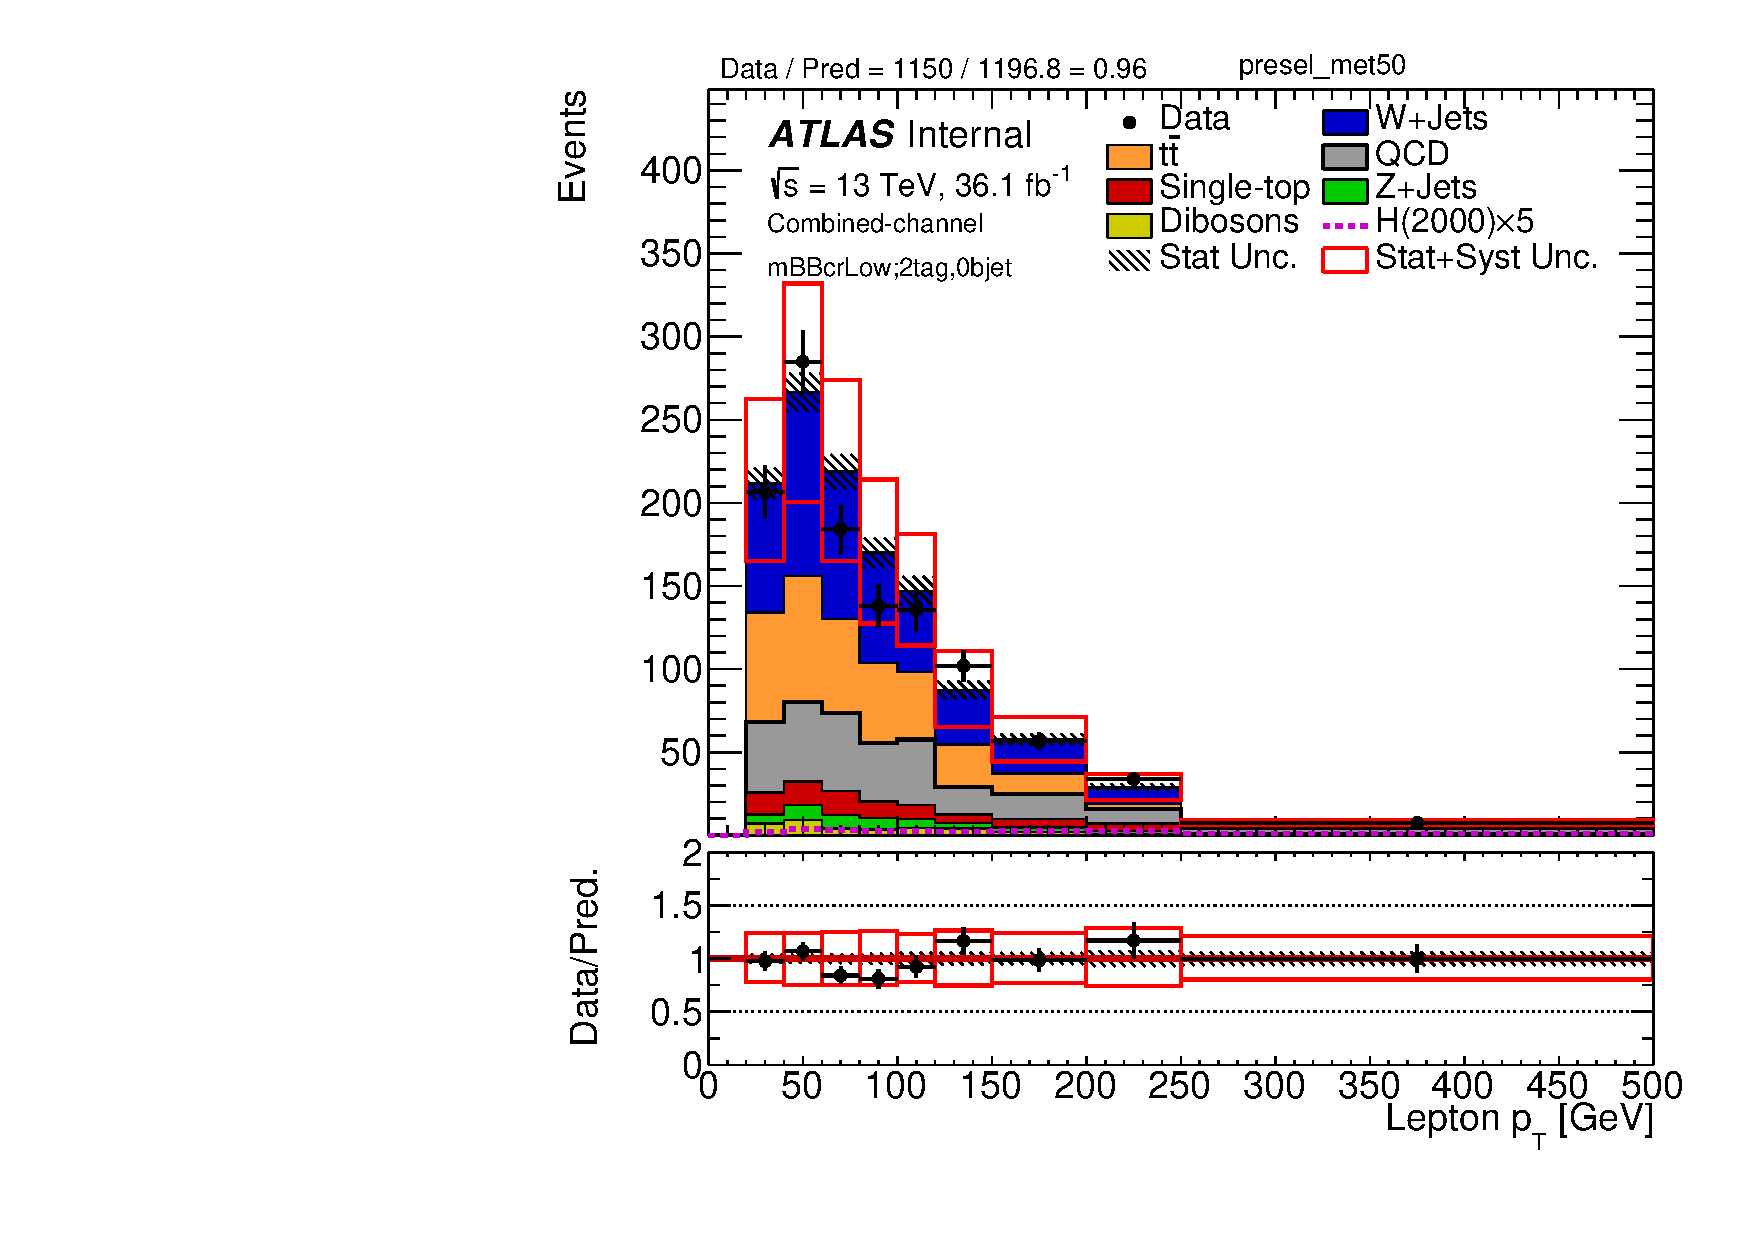
\includegraphics[scale=0.33]{./figures/boosted/PlotByMbbRegions/DataMC_2tag_0bjet_mbbcrLow_lepton_presel_met50_LepPt}                                                                               
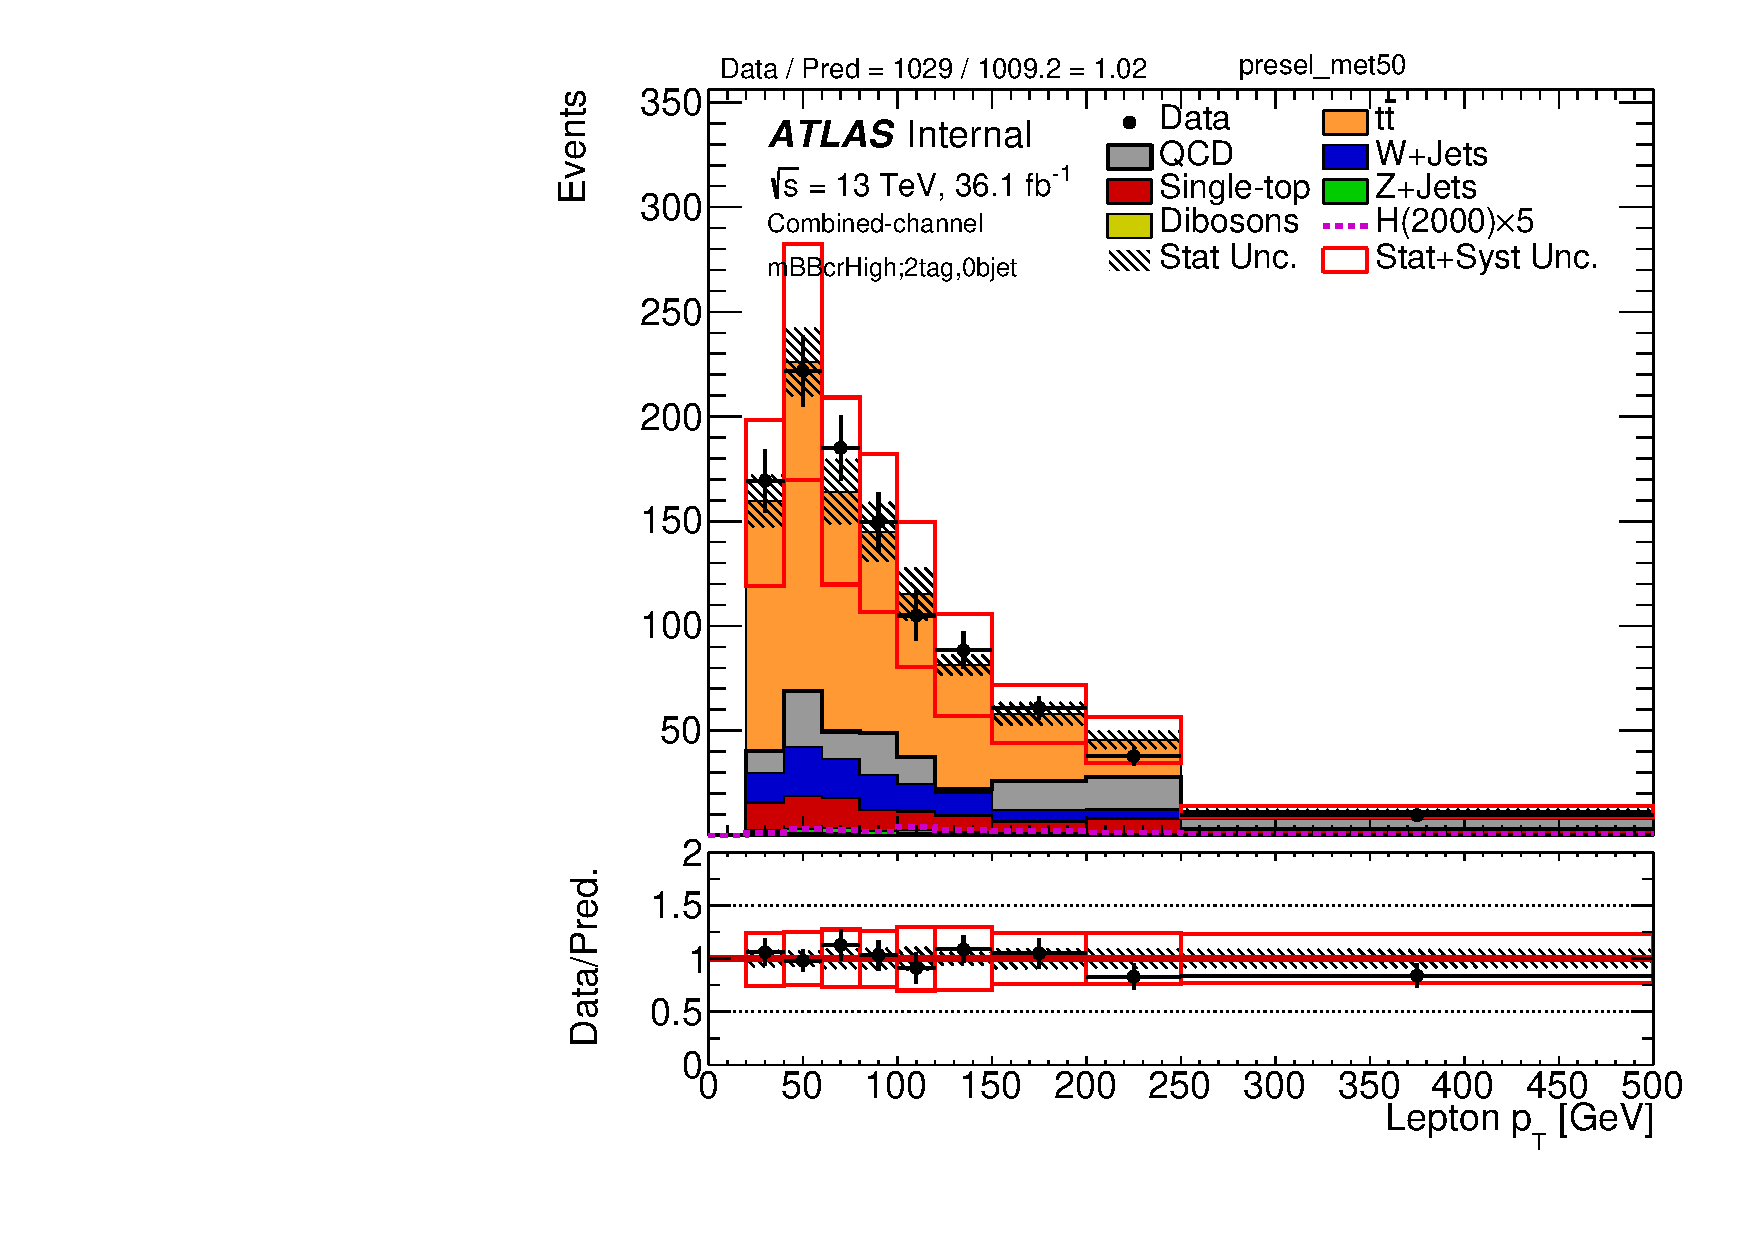
\includegraphics[scale=0.33]{./figures/boosted/PlotByMbbRegions/DataMC_2tag_0bjet_mbbcrHigh_lepton_presel_met50_LepPt}                                                                              
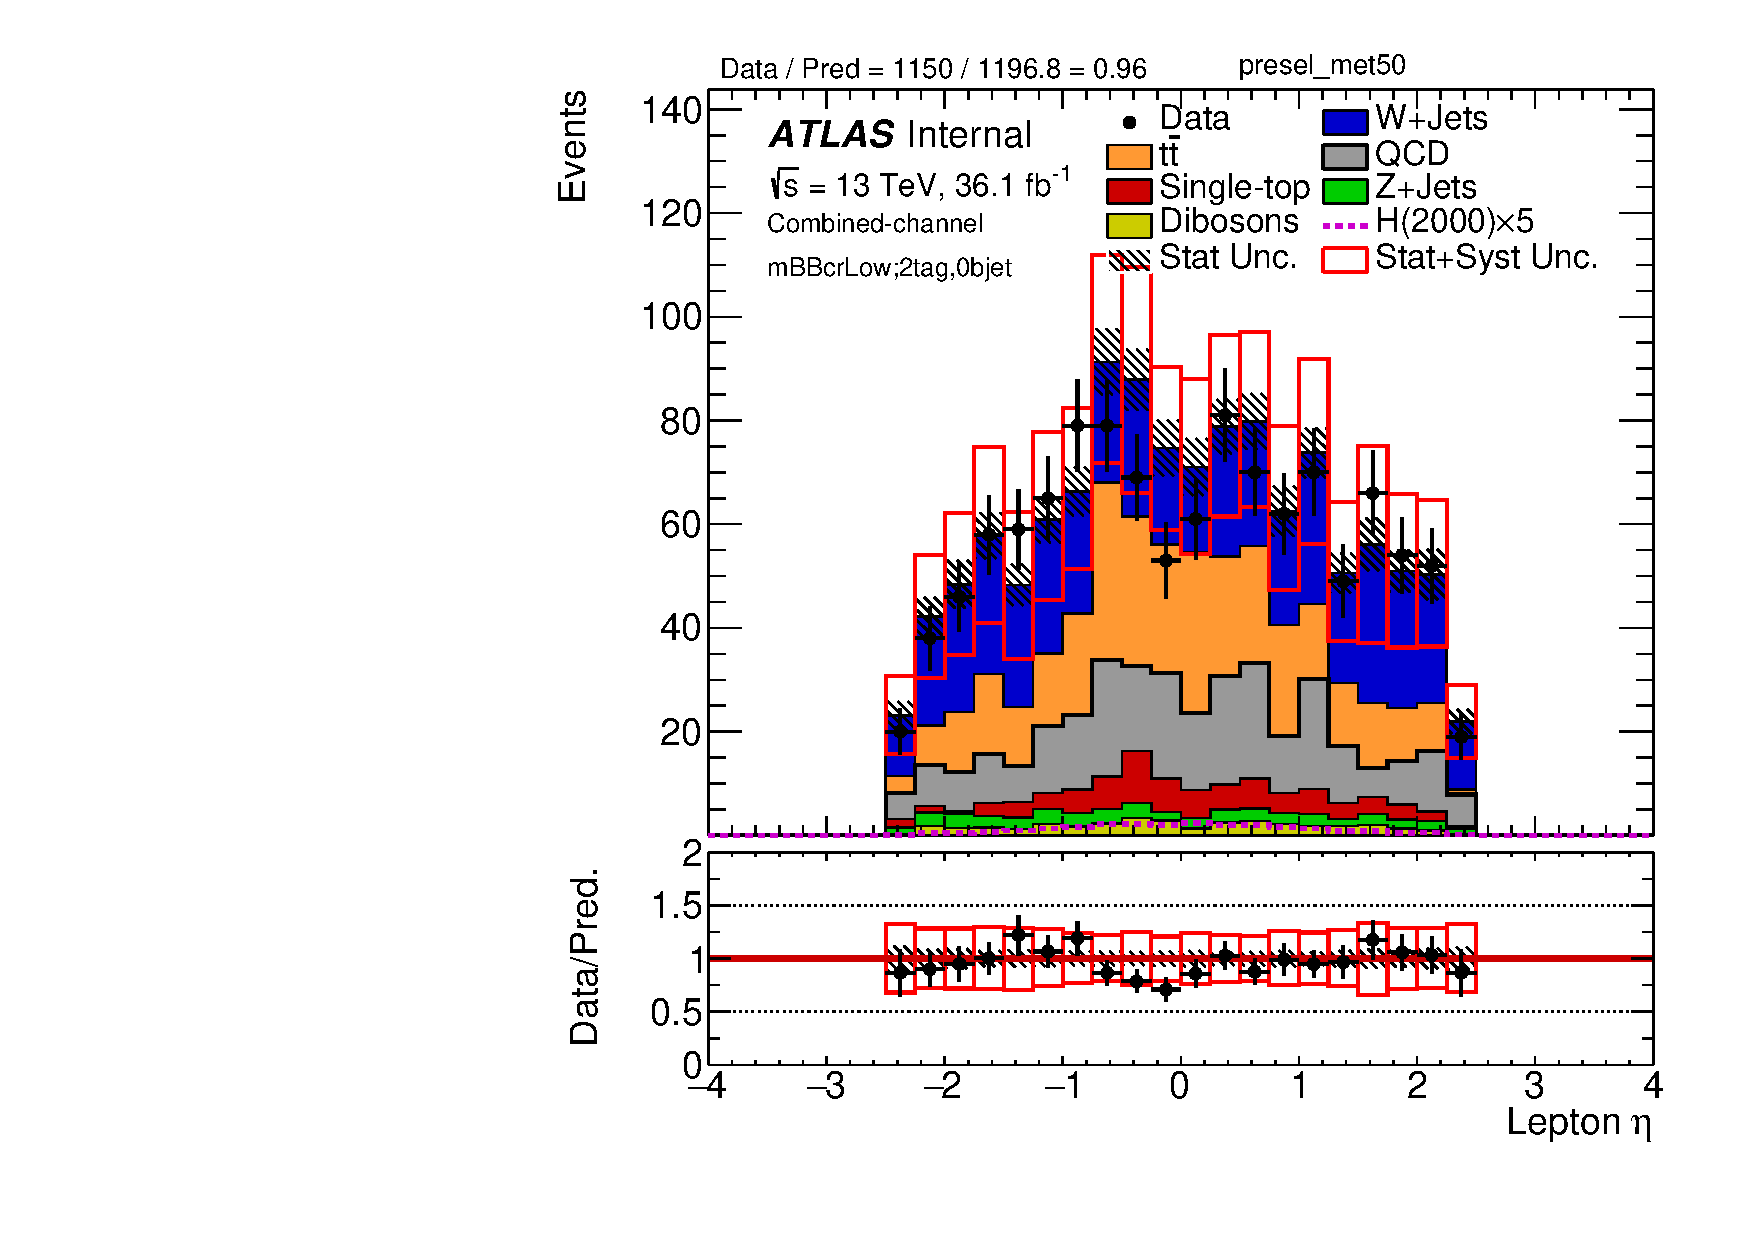
\includegraphics[scale=0.33]{./figures/boosted/PlotByMbbRegions/DataMC_2tag_0bjet_mbbcrLow_lepton_presel_met50_LepEta}                                                                              
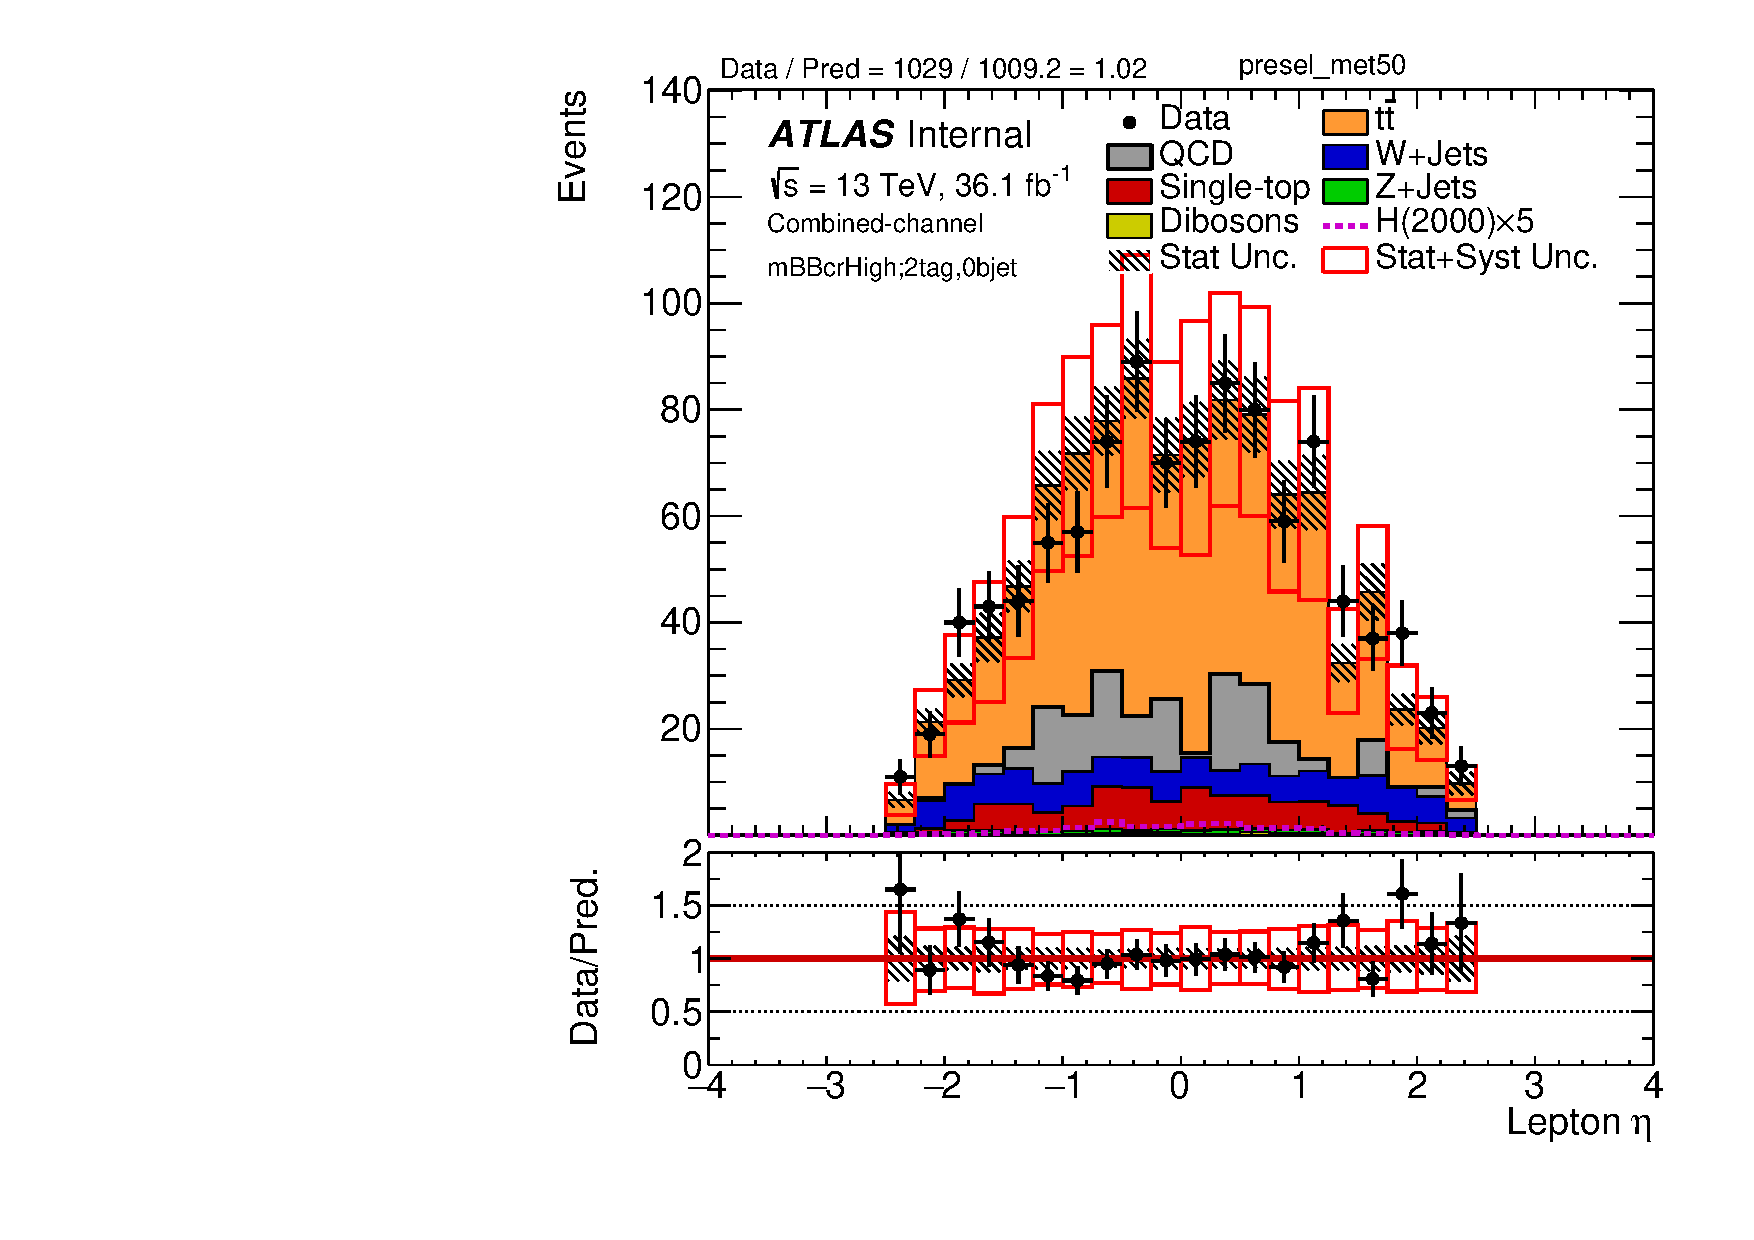
\includegraphics[scale=0.33]{./figures/boosted/PlotByMbbRegions/DataMC_2tag_0bjet_mbbcrHigh_lepton_presel_met50_LepEta}                                                                             
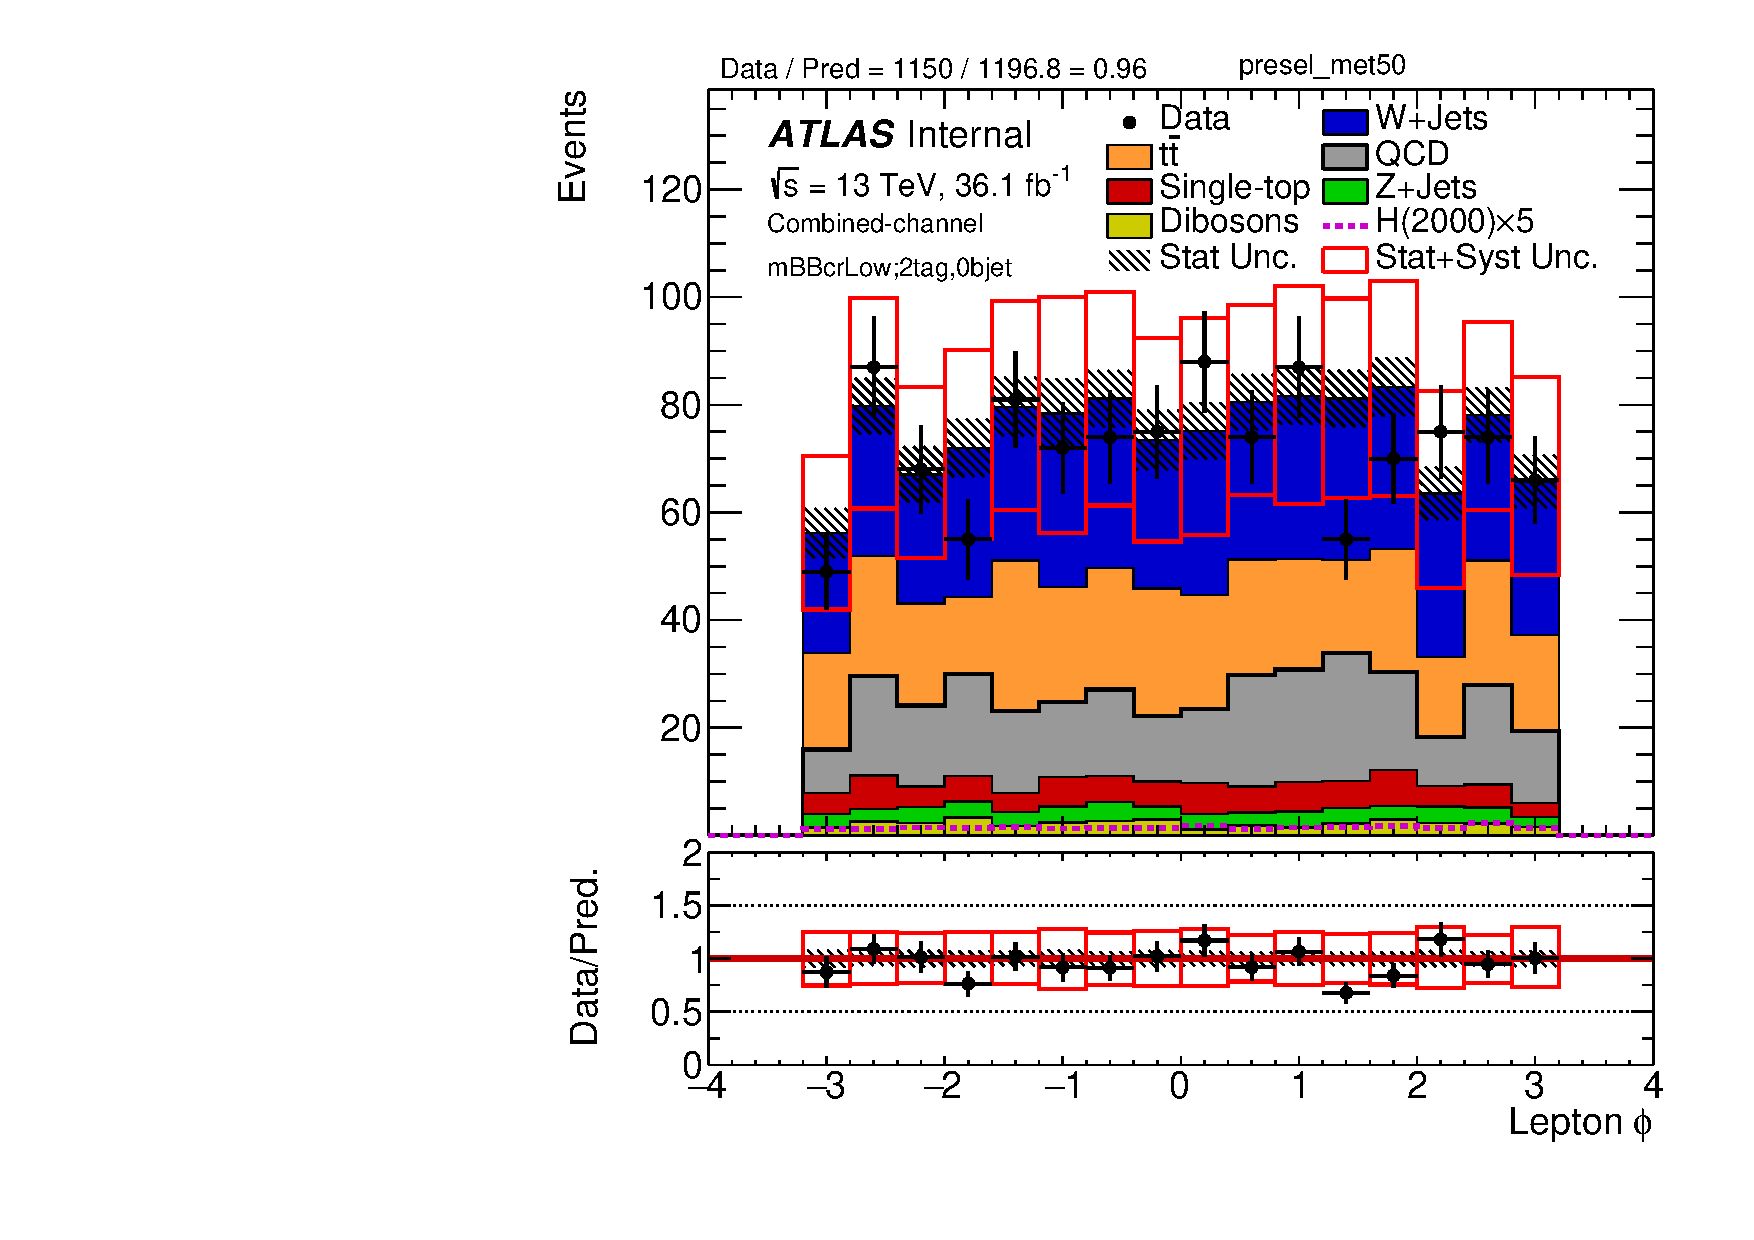
\includegraphics[scale=0.33]{./figures/boosted/PlotByMbbRegions/DataMC_2tag_0bjet_mbbcrLow_lepton_presel_met50_LepPhi}                                                                              
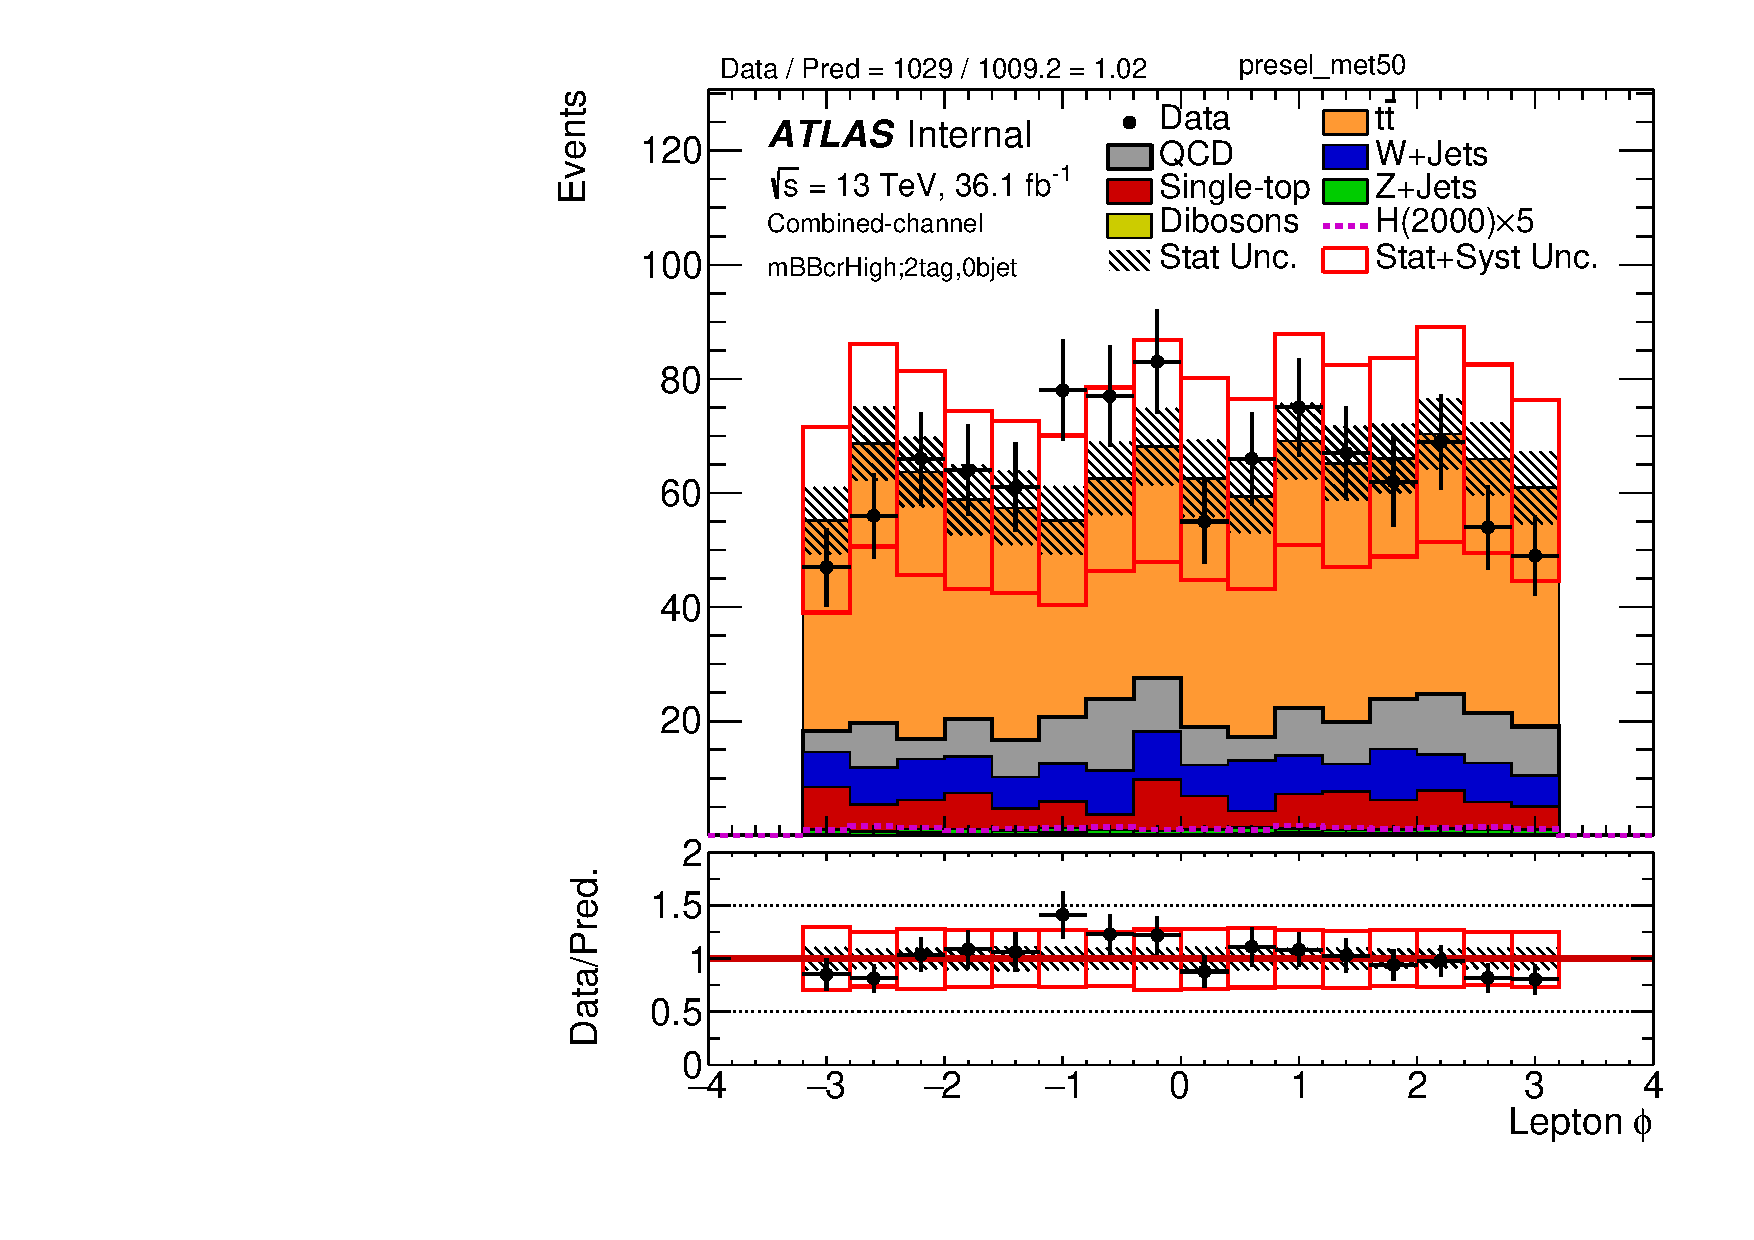
\includegraphics[scale=0.33]{./figures/boosted/PlotByMbbRegions/DataMC_2tag_0bjet_mbbcrHigh_lepton_presel_met50_LepPhi}                                                                             
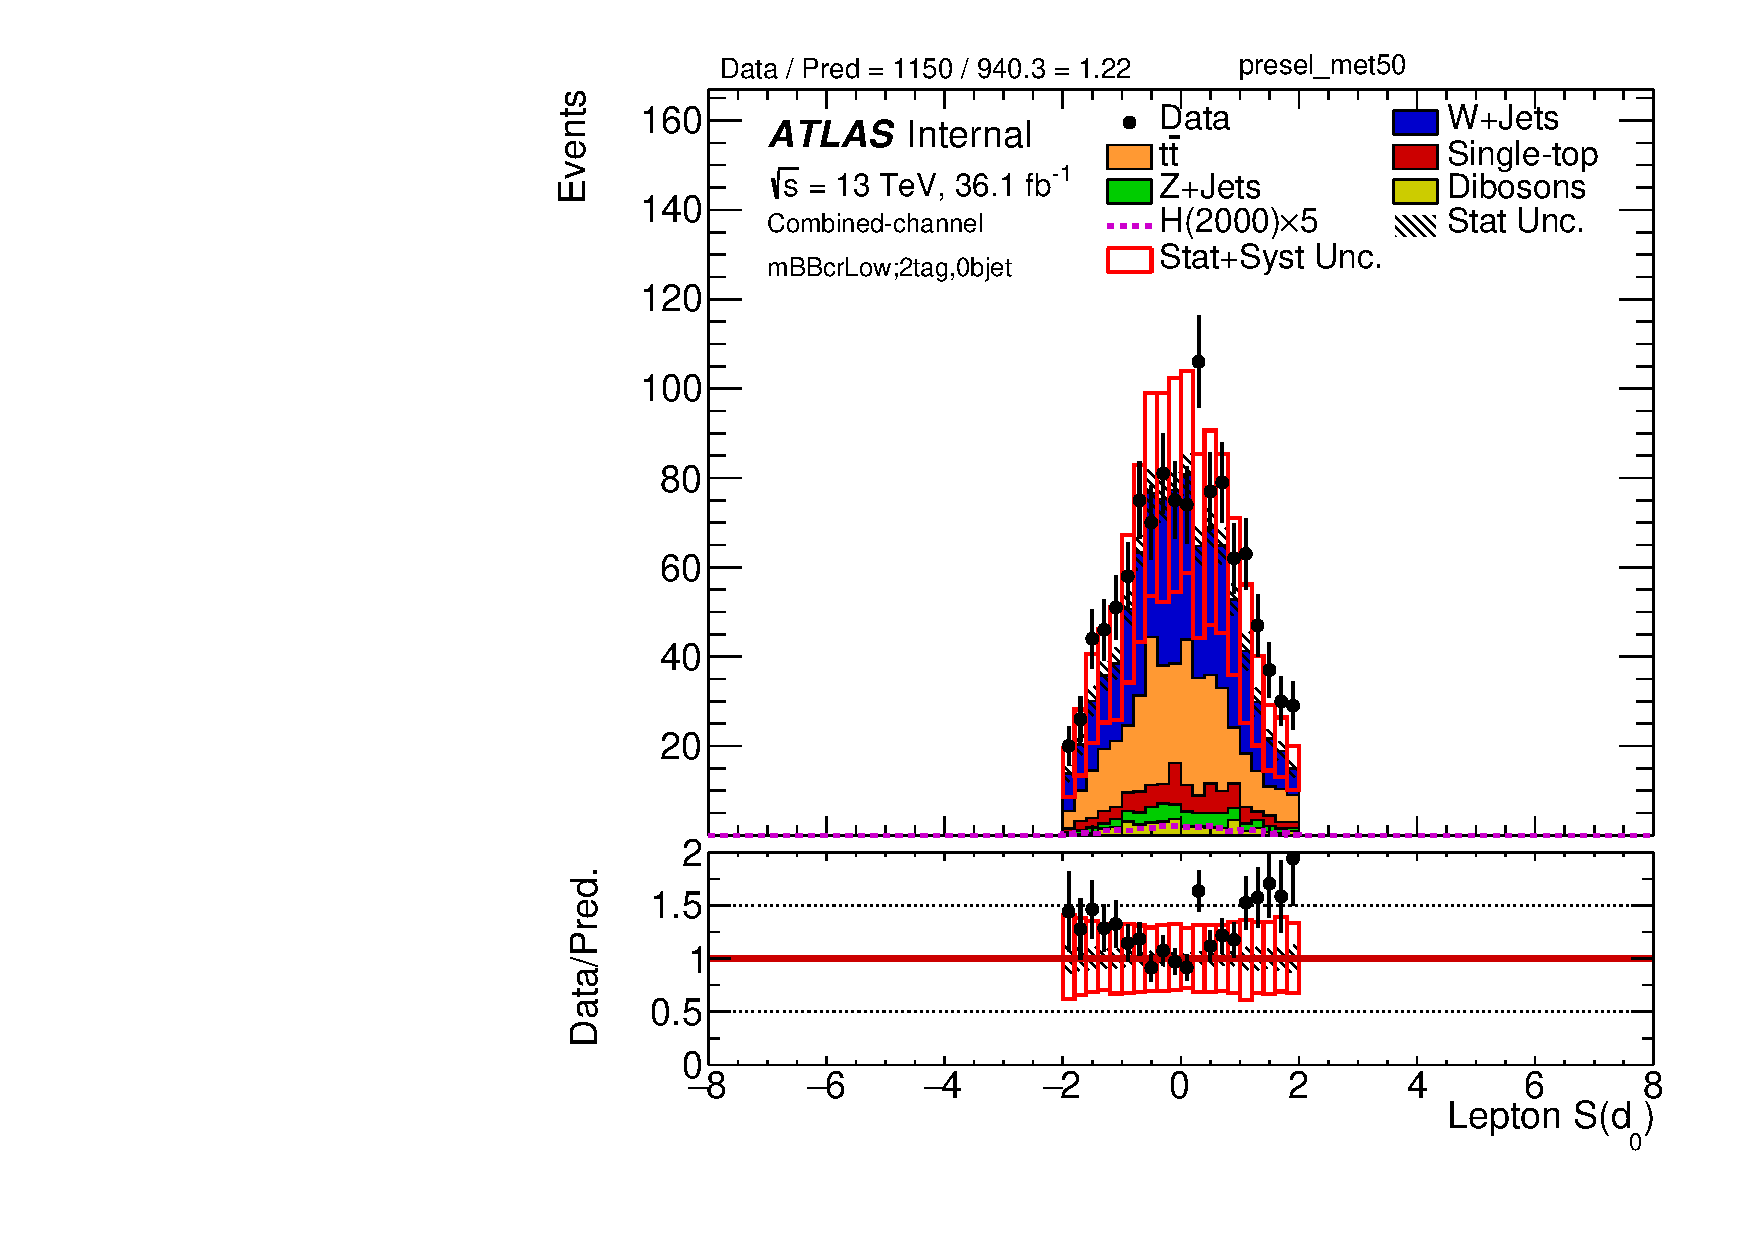
\includegraphics[scale=0.33]{./figures/boosted/PlotByMbbRegions/DataMC_2tag_0bjet_mbbcrLow_lepton_presel_met50_Lep_d0sigL}                                                                          
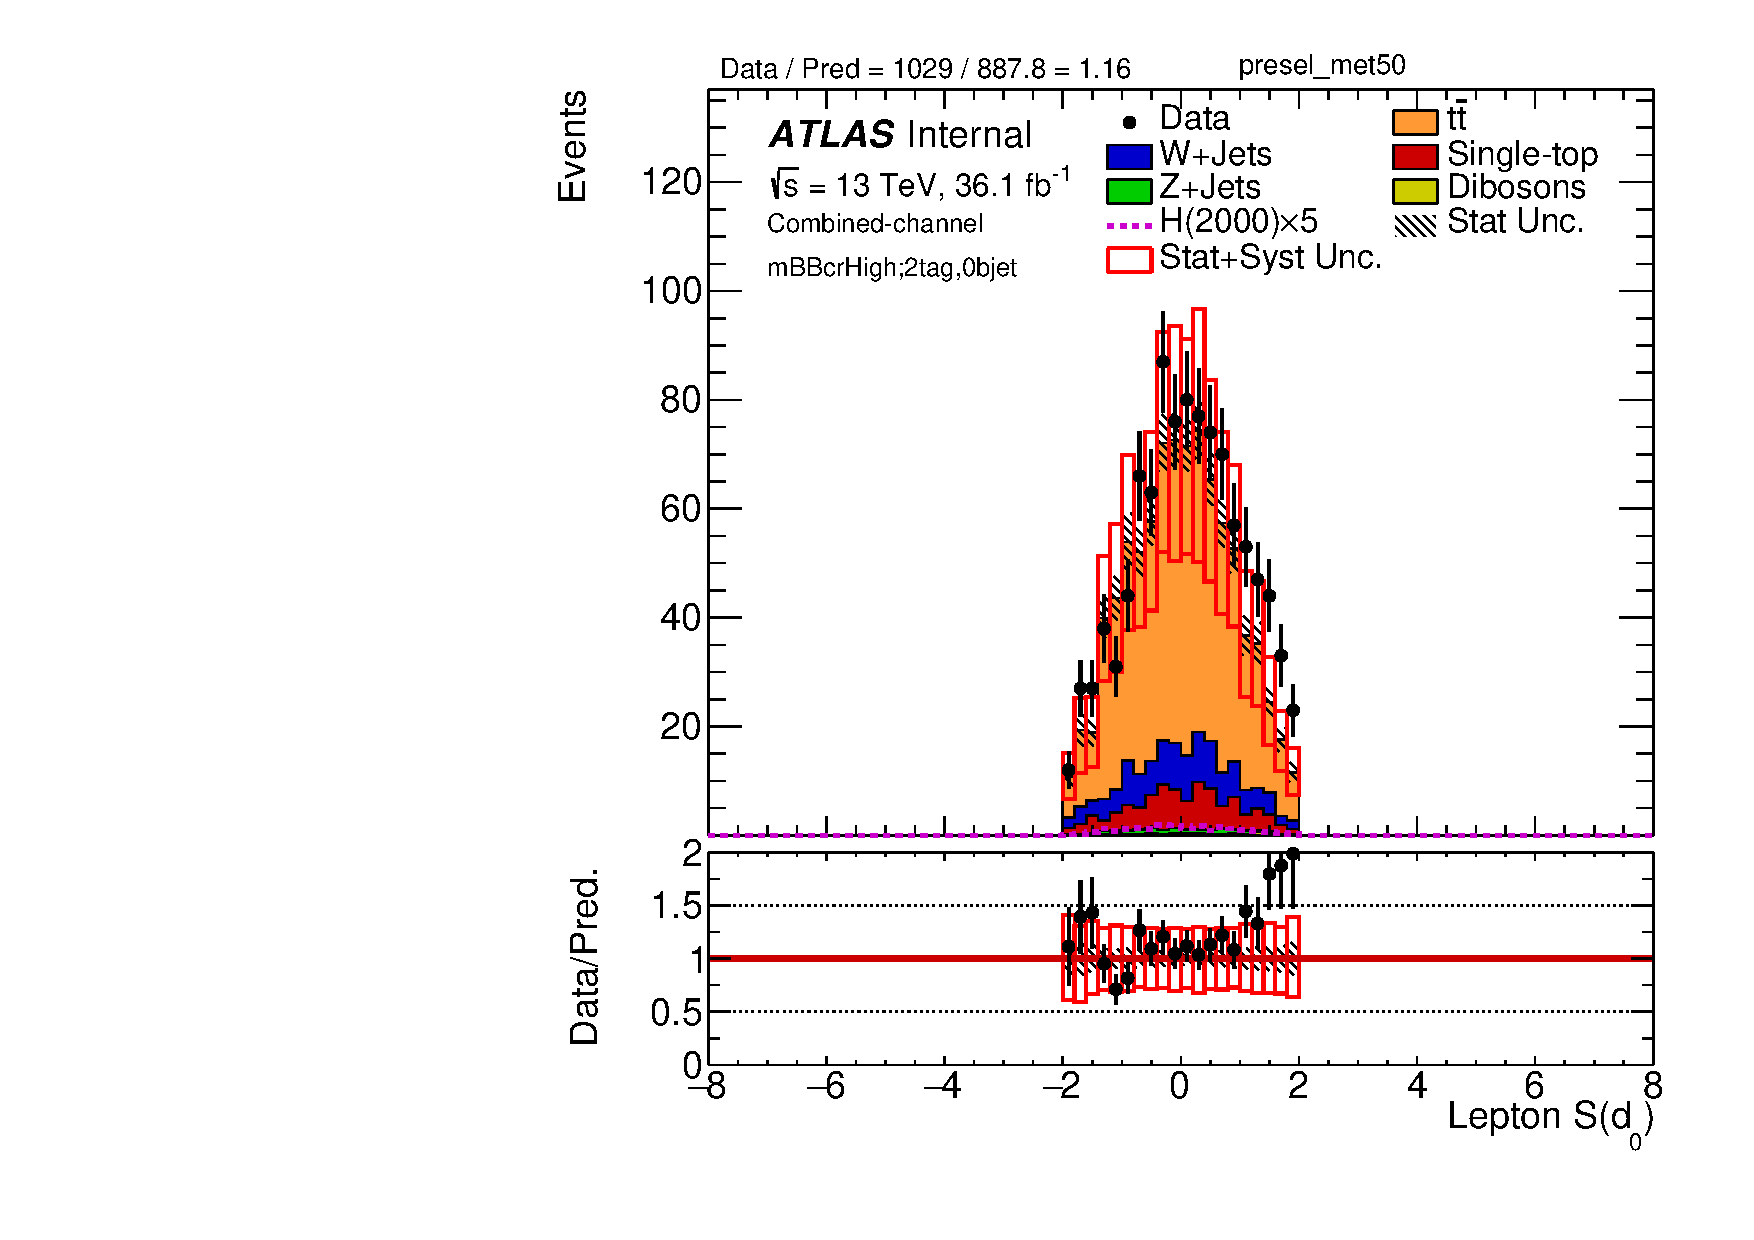
\includegraphics[scale=0.33]{./figures/boosted/PlotByMbbRegions/DataMC_2tag_0bjet_mbbcrHigh_lepton_presel_met50_Lep_d0sigL}                                                                         
\caption{Kinematic distributions of the selected lepton in the low (left) and high (right) mBB control region.}
\label{fig:boosted_mbbcrHighLow_lepton}
\end{center}
\end{figure}

\begin{figure}[!ht]
\begin{center}
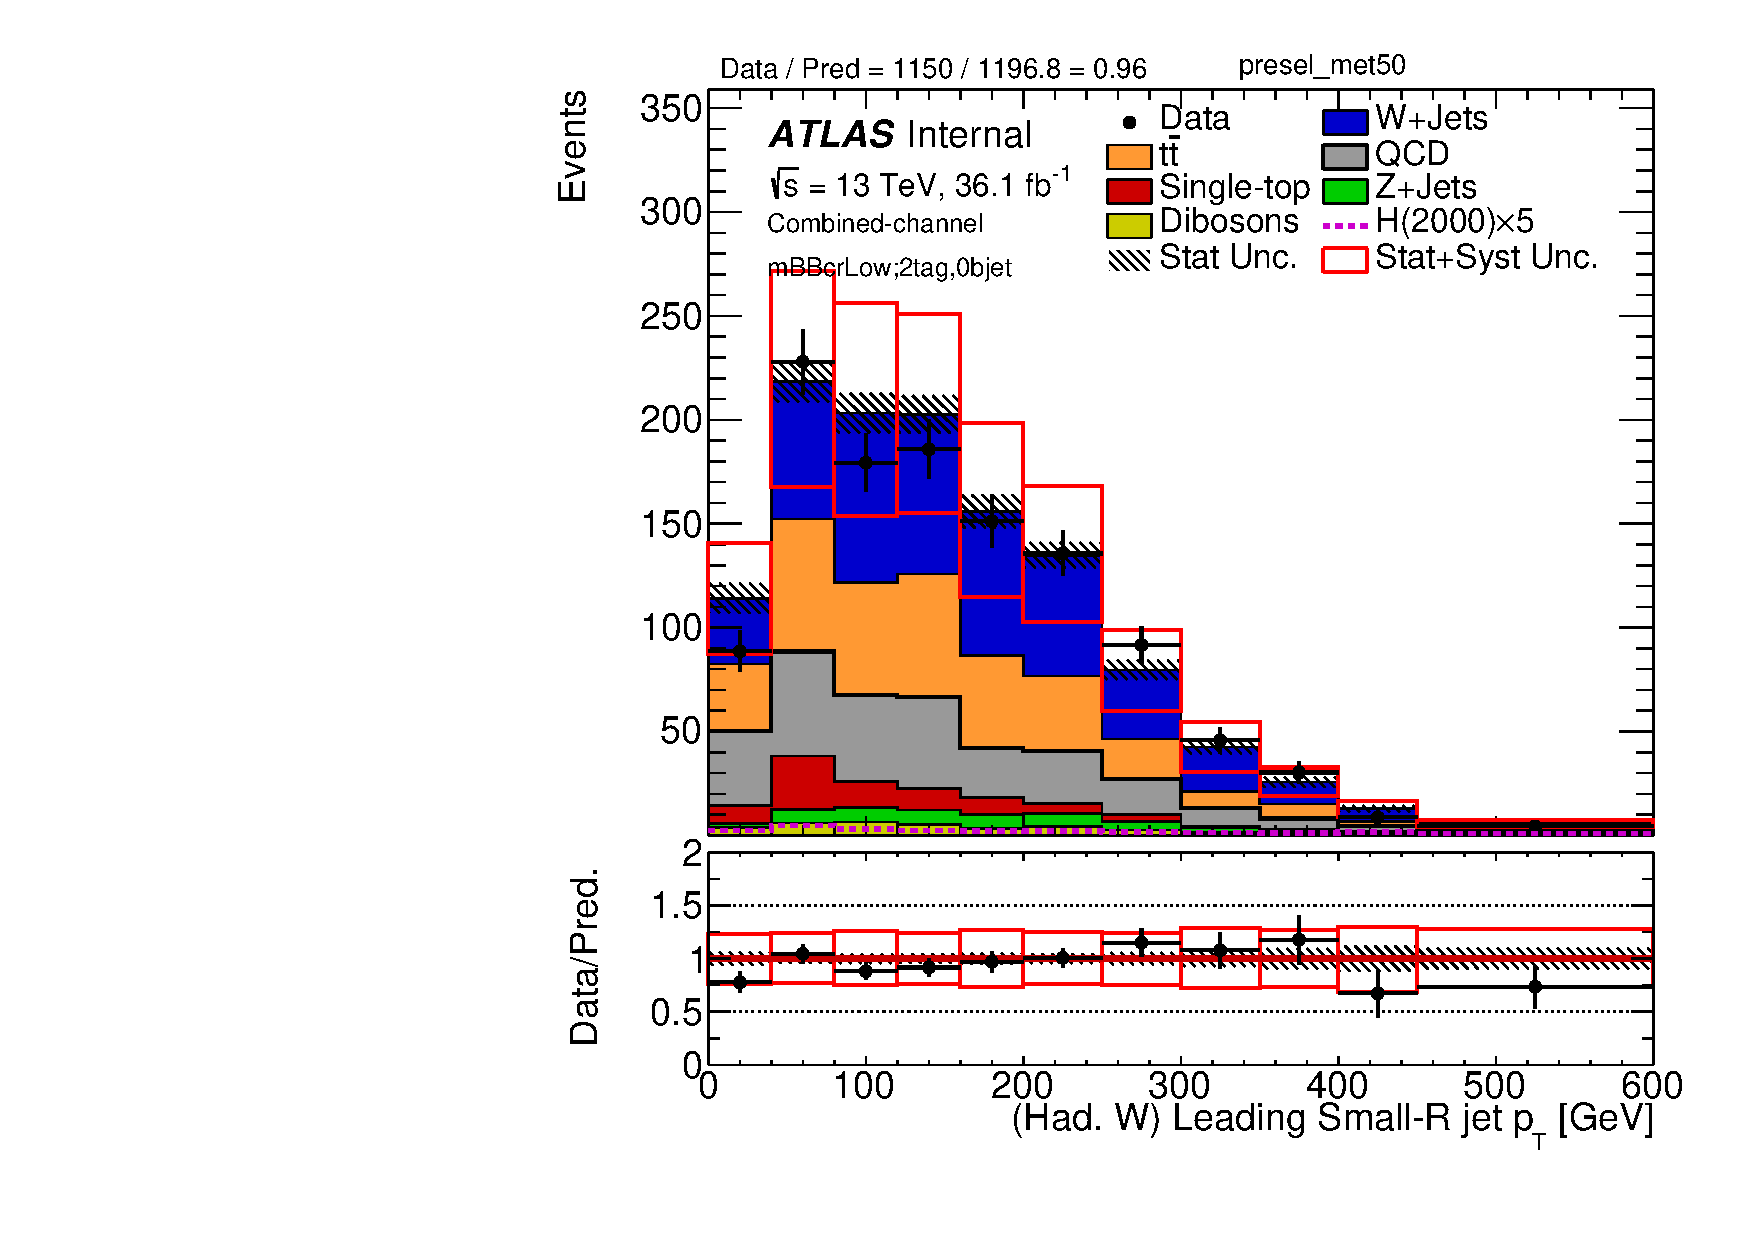
\includegraphics[scale=0.33]{./figures/boosted/PlotByMbbRegions/DataMC_2tag_0bjet_mbbcrLow_lepton_presel_met50_LightJet1Pt}                                                                         
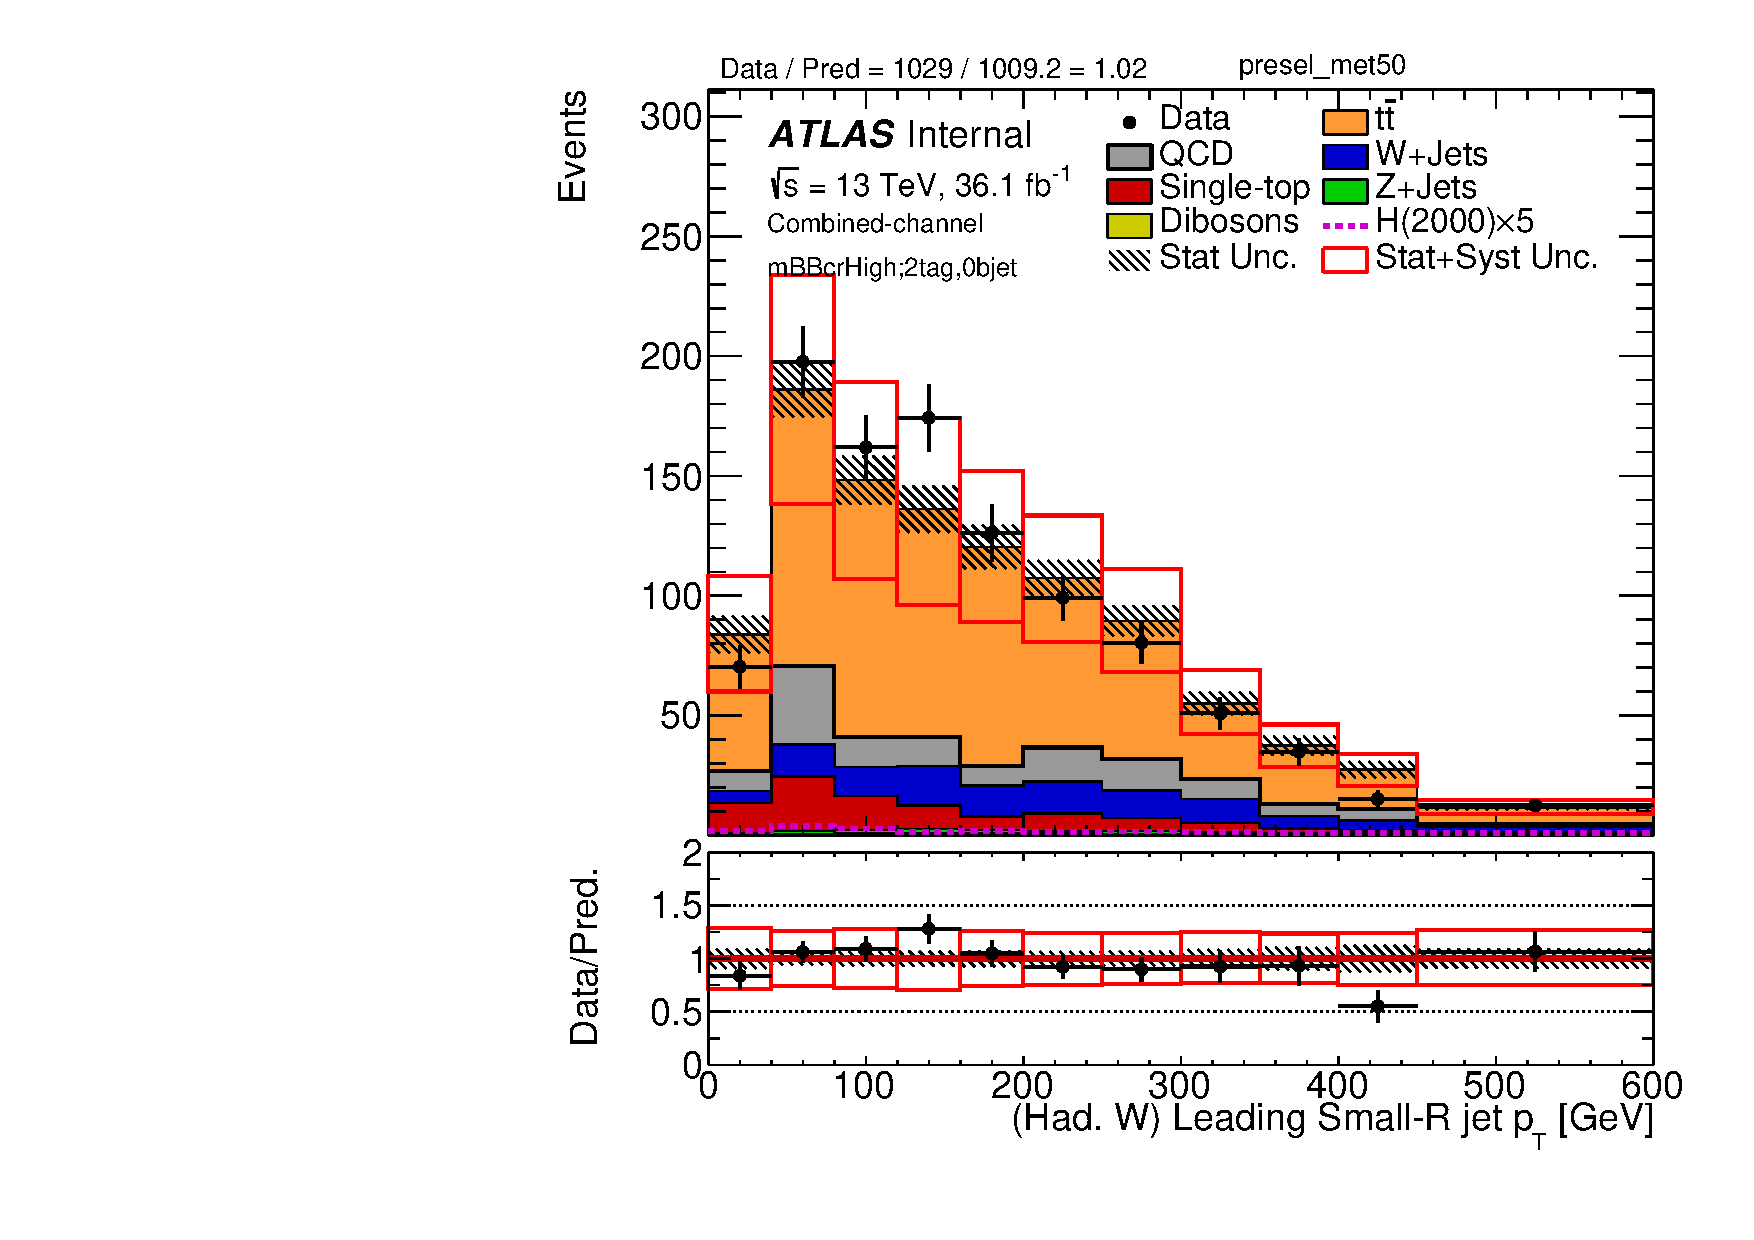
\includegraphics[scale=0.33]{./figures/boosted/PlotByMbbRegions/DataMC_2tag_0bjet_mbbcrHigh_lepton_presel_met50_LightJet1Pt}                                                                        
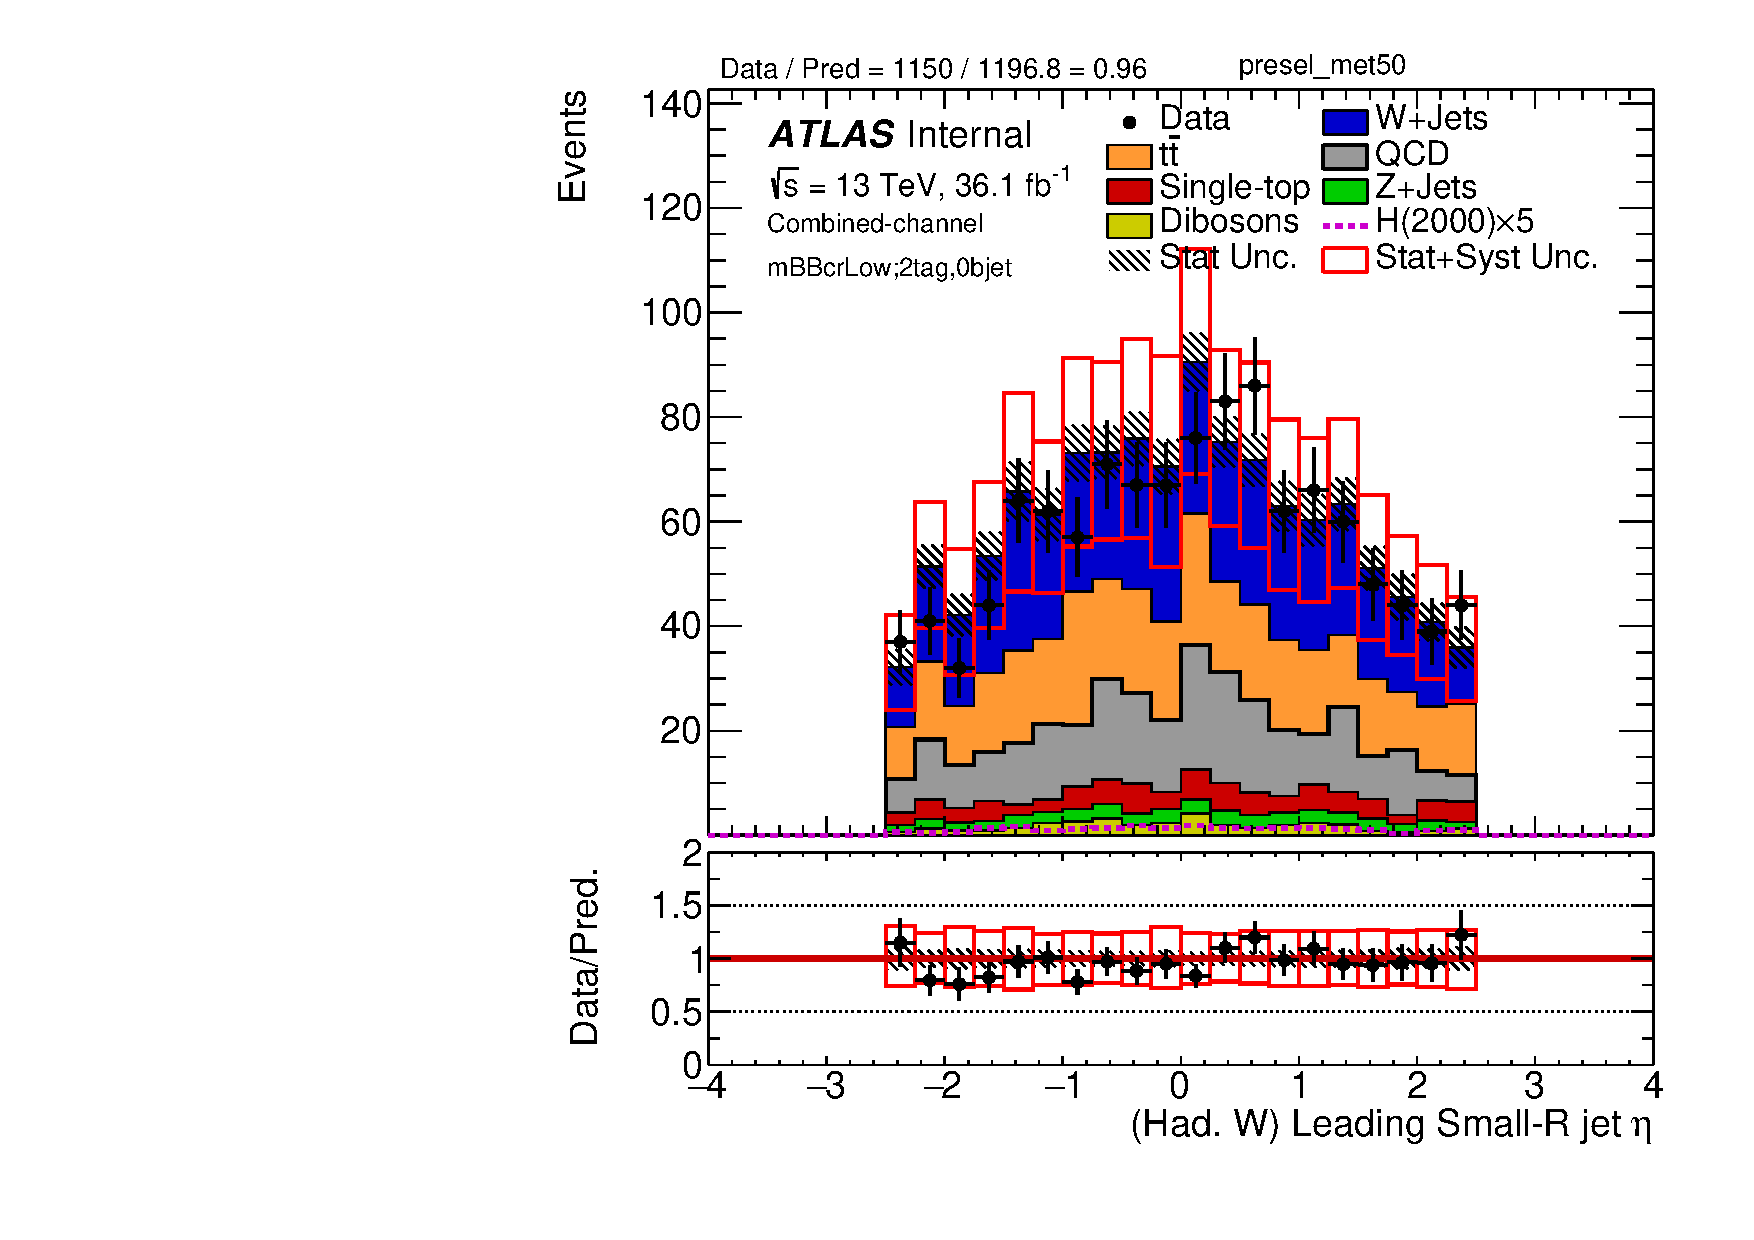
\includegraphics[scale=0.33]{./figures/boosted/PlotByMbbRegions/DataMC_2tag_0bjet_mbbcrLow_lepton_presel_met50_LightJet1Eta}                                                                        
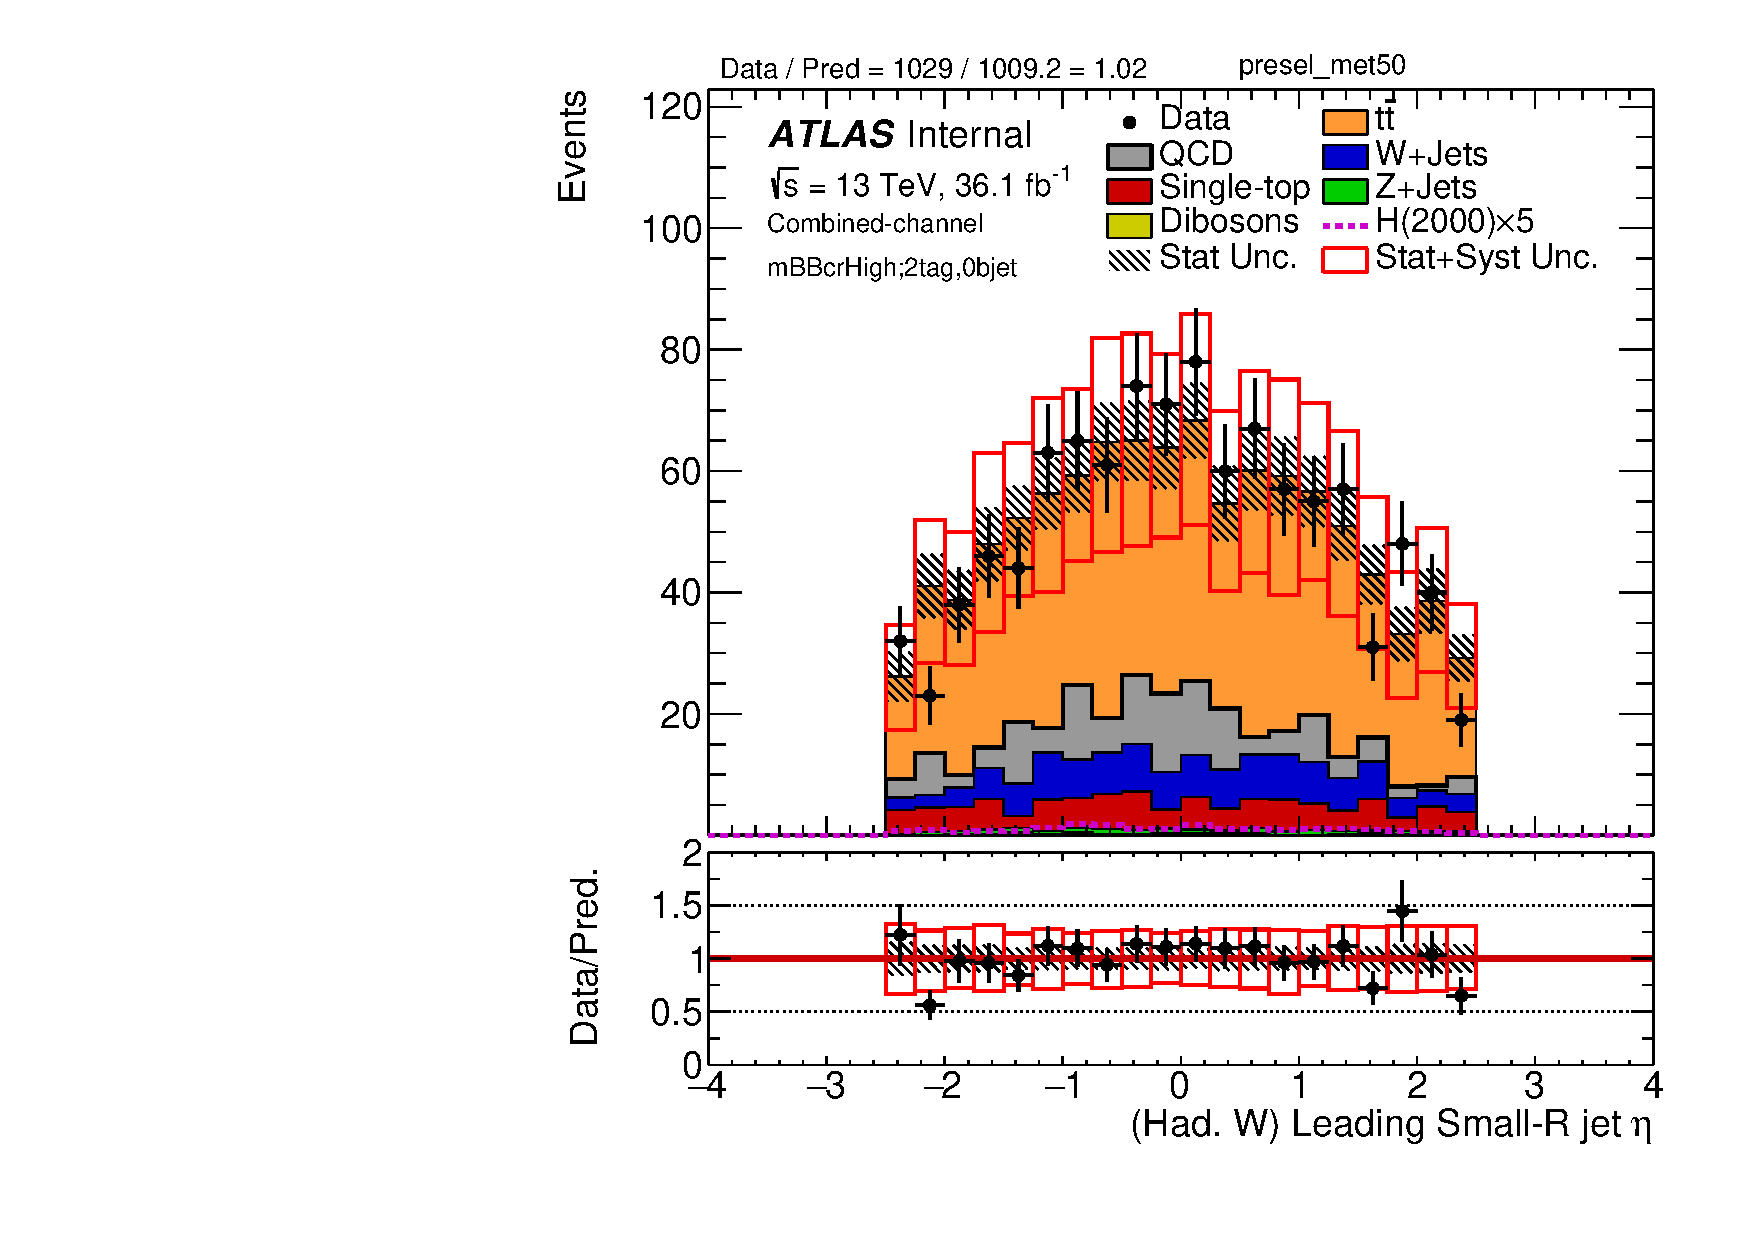
\includegraphics[scale=0.33]{./figures/boosted/PlotByMbbRegions/DataMC_2tag_0bjet_mbbcrHigh_lepton_presel_met50_LightJet1Eta}                                                                       
\includegraphics[scale=0.33]{./figures/boosted/PlotByMbbRegions/DataMC_2tag_0bjet_mbbcrLow_lepton_presel_met50_LightJet1Phi}                                                                        
\includegraphics[scale=0.33]{./figures/boosted/PlotByMbbRegions/DataMC_2tag_0bjet_mbbcrHigh_lepton_presel_met50_LightJet1Phi}                                                                       
\caption{Kinematic distributions of the leading small-$R$ jet (of the reconstructed hadronic W) in the low (left) and high (right) mBB control region.}
\label{fig:boosted_mbbcrHighLow_whad_leadjet}
\end{center}
\end{figure}


\begin{figure}[!ht]
\begin{center}
\includegraphics[scale=0.33]{./figures/boosted/PlotByMbbRegions/DataMC_2tag_0bjet_mbbcrLow_lepton_presel_met50_LightJet2Pt}                                                                         
\includegraphics[scale=0.33]{./figures/boosted/PlotByMbbRegions/DataMC_2tag_0bjet_mbbcrHigh_lepton_presel_met50_LightJet2Pt}                                                                        
\includegraphics[scale=0.33]{./figures/boosted/PlotByMbbRegions/DataMC_2tag_0bjet_mbbcrLow_lepton_presel_met50_LightJet2Eta}                                                                        
\includegraphics[scale=0.33]{./figures/boosted/PlotByMbbRegions/DataMC_2tag_0bjet_mbbcrHigh_lepton_presel_met50_LightJet2Eta}                                                                       
\includegraphics[scale=0.33]{./figures/boosted/PlotByMbbRegions/DataMC_2tag_0bjet_mbbcrLow_lepton_presel_met50_LightJet2Phi}                                                                        
\includegraphics[scale=0.33]{./figures/boosted/PlotByMbbRegions/DataMC_2tag_0bjet_mbbcrHigh_lepton_presel_met50_LightJet2Phi}                                                                       
\caption{Kinematic distributions of the sub-leading small-$R$ jets (of the reconstructed hadronic W) in the low mBB control region low (left) and high (right) mBB control region.}
\label{fig:boosted_mbbcrHighLow_whad_subleadjets}
\end{center}
\end{figure}

\FloatBarrier
%%%%%%%%%%%%%%%%%%%%%%%%%%%%%%%
%
%
%
%
%%%%%%%%%%%%%%%%%%%%%%%%%%%%%%%%
\subsection{mBB control region in electron and muon channels}
\label{app:boosted_mbbcontrolregion_leptonchannels}

Figure~\ref{fig:boosted_mbbcrleptons_mainplots}, \ref{fig:boosted_mbbcrleptons_largerjet}, \ref{fig:boosted_mbbcrleptons_wwsystem},
\ref{fig:boosted_mbbcrleptons_whad}, \ref{fig:boosted_mbbcrleptons_wlep}, \ref{fig:boosted_mbbcrleptons_lepton}, \ref{fig:boosted_mbbcrleptons_whad_leadjet},
\ref{fig:boosted_mbbcrleptons_whad_subleadjets} and \ref{fig:boosted_mbbcrleptons_whad_dr} shows the kinematic distribution of events 
in the electron channel and the muon channel in the mBB control region.

\begin{figure}[!h]
\begin{center}
\includegraphics[scale=0.33]{./figures/boosted/PlotByChannels/DataMC_2tag_0bjet_mbbcr_elec_presel_met50_hhMassRebin1}                                                                               
\includegraphics[scale=0.33]{./figures/boosted/PlotByChannels/DataMC_2tag_0bjet_mbbcr_muon_presel_met50_hhMassRebin1}                                                                               
\includegraphics[scale=0.33]{./figures/boosted/PlotByChannels/DataMC_2tag_0bjet_mbbcr_elec_presel_met50_MET}                                                                                        
\includegraphics[scale=0.33]{./figures/boosted/PlotByChannels/DataMC_2tag_0bjet_mbbcr_muon_presel_met50_MET}                                                                                        
\includegraphics[scale=0.33]{./figures/boosted/PlotByChannels/DataMC_2tag_0bjet_mbbcr_elec_presel_met50_WlepMtATLAS}                                                                                
\includegraphics[scale=0.33]{./figures/boosted/PlotByChannels/DataMC_2tag_0bjet_mbbcr_muon_presel_met50_WlepMtATLAS}                                                                                
\caption{The invariant mass of the reconstructed di-Higgs (hh) system, \met and transverse mass of the $W \to l\nu$ system 
distributions of events in the mBB control region of the electron (left) and muon (right) channel.}
\label{fig:boosted_mbbcrleptons_mainplots}
\end{center}
\end{figure}

\begin{figure}[!h]
\begin{center}
\includegraphics[scale=0.33]{./figures/boosted/PlotByChannels/DataMC_2tag_0bjet_mbbcr_elec_presel_met50_HbbPt}                                                                                      
\includegraphics[scale=0.33]{./figures/boosted/PlotByChannels/DataMC_2tag_0bjet_mbbcr_muon_presel_met50_HbbPt}                                                                                      
\includegraphics[scale=0.33]{./figures/boosted/PlotByChannels/DataMC_2tag_0bjet_mbbcr_elec_presel_met50_HbbMass}                                                                                    
\includegraphics[scale=0.33]{./figures/boosted/PlotByChannels/DataMC_2tag_0bjet_mbbcr_muon_presel_met50_HbbMass}                                                                                    
\includegraphics[scale=0.33]{./figures/boosted/PlotByChannels/DataMC_2tag_0bjet_mbbcr_elec_presel_met50_HbbEta}                                                              
\includegraphics[scale=0.33]{./figures/boosted/PlotByChannels/DataMC_2tag_0bjet_mbbcr_muon_presel_met50_HbbEta}                                                              
\includegraphics[scale=0.33]{./figures/boosted/PlotByChannels/DataMC_2tag_0bjet_mbbcr_elec_presel_met50_HbbPhi}                                                              
\includegraphics[scale=0.33]{./figures/boosted/PlotByChannels/DataMC_2tag_0bjet_mbbcr_muon_presel_met50_HbbPhi}                                                              
\caption{Kinematic distributions of the reconstructed large-$R$ jet in the mBB control region of the electron (left) and muon (right) channel.}
\label{fig:boosted_mbbcrleptons_largerjet}
\end{center}
\end{figure}

\begin{figure}[!h]
\begin{center}
\includegraphics[scale=0.33]{./figures/boosted/PlotByChannels/DataMC_2tag_0bjet_mbbcr_elec_presel_met50_WWPt}                                                                                       
\includegraphics[scale=0.33]{./figures/boosted/PlotByChannels/DataMC_2tag_0bjet_mbbcr_muon_presel_met50_WWPt}                                                                                       
\includegraphics[scale=0.33]{./figures/boosted/PlotByChannels/DataMC_2tag_0bjet_mbbcr_elec_presel_met50_WWMass}                                                                                     
\includegraphics[scale=0.33]{./figures/boosted/PlotByChannels/DataMC_2tag_0bjet_mbbcr_muon_presel_met50_WWMass}                                                                                     
\includegraphics[scale=0.33]{./figures/boosted/PlotByChannels/DataMC_2tag_0bjet_mbbcr_elec_presel_met50_WWEta}                                                                                      
\includegraphics[scale=0.33]{./figures/boosted/PlotByChannels/DataMC_2tag_0bjet_mbbcr_muon_presel_met50_WWEta}                                                                                      
\includegraphics[scale=0.33]{./figures/boosted/PlotByChannels/DataMC_2tag_0bjet_mbbcr_elec_presel_met50_WWPhi}                                                                                      
\includegraphics[scale=0.33]{./figures/boosted/PlotByChannels/DataMC_2tag_0bjet_mbbcr_muon_presel_met50_WWPhi}                                                                                      
\caption{Kinematic distributions of the reconstructed $h \to WW$ system in the mBB control region of the electron (left) and muon (right) channel.}
\label{fig:boosted_mbbcrleptons_wwsystem}
\end{center}
\end{figure}

\begin{figure}[!h]
\begin{center}
\includegraphics[scale=0.33]{./figures/boosted/PlotByChannels/DataMC_2tag_0bjet_mbbcr_elec_presel_met50_WhadPt}  
\includegraphics[scale=0.33]{./figures/boosted/PlotByChannels/DataMC_2tag_0bjet_mbbcr_muon_presel_met50_WhadPt}  
\includegraphics[scale=0.33]{./figures/boosted/PlotByChannels/DataMC_2tag_0bjet_mbbcr_elec_presel_met50_WhadMass}
\includegraphics[scale=0.33]{./figures/boosted/PlotByChannels/DataMC_2tag_0bjet_mbbcr_muon_presel_met50_WhadMass}
\includegraphics[scale=0.33]{./figures/boosted/PlotByChannels/DataMC_2tag_0bjet_mbbcr_elec_presel_met50_WhadEta} 
\includegraphics[scale=0.33]{./figures/boosted/PlotByChannels/DataMC_2tag_0bjet_mbbcr_muon_presel_met50_WhadEta} 
\includegraphics[scale=0.33]{./figures/boosted/PlotByChannels/DataMC_2tag_0bjet_mbbcr_elec_presel_met50_WhadPhi} 
\includegraphics[scale=0.33]{./figures/boosted/PlotByChannels/DataMC_2tag_0bjet_mbbcr_muon_presel_met50_WhadPhi} 
\caption{Kinematic distributions of the reconstructed $W \to q\bar{q}$ system in the mBB control region of the electron (left) and muon (right) channel.}
\label{fig:boosted_mbbcrleptons_whad}
\end{center}
\end{figure}

\begin{figure}[!h]
\begin{center}
\includegraphics[scale=0.33]{./figures/boosted/PlotByChannels/DataMC_2tag_0bjet_mbbcr_elec_presel_met50_WlepPt}  
\includegraphics[scale=0.33]{./figures/boosted/PlotByChannels/DataMC_2tag_0bjet_mbbcr_muon_presel_met50_WlepPt}  
\includegraphics[scale=0.33]{./figures/boosted/PlotByChannels/DataMC_2tag_0bjet_mbbcr_elec_presel_met50_WlepMass}
\includegraphics[scale=0.33]{./figures/boosted/PlotByChannels/DataMC_2tag_0bjet_mbbcr_muon_presel_met50_WlepMass}
\includegraphics[scale=0.33]{./figures/boosted/PlotByChannels/DataMC_2tag_0bjet_mbbcr_elec_presel_met50_WlepEta} 
\includegraphics[scale=0.33]{./figures/boosted/PlotByChannels/DataMC_2tag_0bjet_mbbcr_muon_presel_met50_WlepEta} 
\includegraphics[scale=0.33]{./figures/boosted/PlotByChannels/DataMC_2tag_0bjet_mbbcr_elec_presel_met50_WlepPhi} 
\includegraphics[scale=0.33]{./figures/boosted/PlotByChannels/DataMC_2tag_0bjet_mbbcr_muon_presel_met50_WlepPhi} 
\caption{Kinematic distributions of the reconstructed $W \to l\nu$ system in the mBB control region of the electron (left) and muon (right) channel.}`
\label{fig:boosted_mbbcrleptons_wlep}
\end{center}
\end{figure}

\begin{figure}[!h]
\begin{center}
\includegraphics[scale=0.33]{./figures/boosted/PlotByChannels/DataMC_2tag_0bjet_mbbcr_elec_presel_met50_LepPt} 
\includegraphics[scale=0.33]{./figures/boosted/PlotByChannels/DataMC_2tag_0bjet_mbbcr_muon_presel_met50_LepPt} 
\includegraphics[scale=0.33]{./figures/boosted/PlotByChannels/DataMC_2tag_0bjet_mbbcr_elec_presel_met50_LepEta}                                                                                     
\includegraphics[scale=0.33]{./figures/boosted/PlotByChannels/DataMC_2tag_0bjet_mbbcr_muon_presel_met50_LepEta}                                                                                     
\includegraphics[scale=0.33]{./figures/boosted/PlotByChannels/DataMC_2tag_0bjet_mbbcr_elec_presel_met50_LepPhi}                                                                                     
\includegraphics[scale=0.33]{./figures/boosted/PlotByChannels/DataMC_2tag_0bjet_mbbcr_muon_presel_met50_LepPhi}                                                                                     
\includegraphics[scale=0.33]{./figures/boosted/PlotByChannels/DataMC_2tag_0bjet_mbbcr_elec_presel_met50_Lep_d0sigL}                                                                                 
\includegraphics[scale=0.33]{./figures/boosted/PlotByChannels/DataMC_2tag_0bjet_mbbcr_muon_presel_met50_Lep_d0sigL}                                                                                 
\caption{Kinematic distributions of the selected lepton in the mBB control region of the electron (left) and muon (right) channel.}
\label{fig:boosted_mbbcrleptons_lepton}
\end{center}
\end{figure}

\begin{figure}[!ht]
\begin{center}
\includegraphics[scale=0.33]{./figures/boosted/PlotByChannels/DataMC_2tag_0bjet_mbbcr_elec_presel_met50_LightJet1Pt} 
\includegraphics[scale=0.33]{./figures/boosted/PlotByChannels/DataMC_2tag_0bjet_mbbcr_muon_presel_met50_LightJet1Pt} 
\includegraphics[scale=0.33]{./figures/boosted/PlotByChannels/DataMC_2tag_0bjet_mbbcr_elec_presel_met50_LightJet1Eta}                                                                               
\includegraphics[scale=0.33]{./figures/boosted/PlotByChannels/DataMC_2tag_0bjet_mbbcr_muon_presel_met50_LightJet1Eta}                                                                               
\includegraphics[scale=0.33]{./figures/boosted/PlotByChannels/DataMC_2tag_0bjet_mbbcr_elec_presel_met50_LightJet1Phi}                                                                               
\includegraphics[scale=0.33]{./figures/boosted/PlotByChannels/DataMC_2tag_0bjet_mbbcr_muon_presel_met50_LightJet1Phi}                                                                               
\caption{Kinematic distributions of the leading small-$R$ jet (of the reconstructed hadronic W) in the mBB control region of the electron (left) 
and muon (right) channel.}
\label{fig:boosted_mbbcrleptons_whad_leadjet}
\end{center}
\end{figure}


\begin{figure}[!ht]
\begin{center}
\includegraphics[scale=0.33]{./figures/boosted/PlotByChannels/DataMC_2tag_0bjet_mbbcr_elec_presel_met50_LightJet2Pt}
\includegraphics[scale=0.33]{./figures/boosted/PlotByChannels/DataMC_2tag_0bjet_mbbcr_muon_presel_met50_LightJet2Pt}
\includegraphics[scale=0.33]{./figures/boosted/PlotByChannels/DataMC_2tag_0bjet_mbbcr_elec_presel_met50_LightJet2Eta}                                                                               
\includegraphics[scale=0.33]{./figures/boosted/PlotByChannels/DataMC_2tag_0bjet_mbbcr_muon_presel_met50_LightJet2Eta}                                                                               
\includegraphics[scale=0.33]{./figures/boosted/PlotByChannels/DataMC_2tag_0bjet_mbbcr_elec_presel_met50_LightJet2Phi}                                                                               
\includegraphics[scale=0.33]{./figures/boosted/PlotByChannels/DataMC_2tag_0bjet_mbbcr_muon_presel_met50_LightJet2Phi}                                                                               
\caption{Kinematic distributions of the sub-leading small-$R$ jets (of the reconstructed hadronic W) in the mBB control region of the electron (left) 
and muon (right) channel.}
\label{fig:boosted_mbbcrleptons_whad_subleadjets}
\end{center}
\end{figure}


\begin{figure}[!h]
\begin{center}
\includegraphics[scale=0.33]{./figures/boosted/PlotByChannels/DataMC_2tag_0bjet_mbbcr_elec_presel_met50_drHbbLep}                                                                                   
\includegraphics[scale=0.33]{./figures/boosted/PlotByChannels/DataMC_2tag_0bjet_mbbcr_muon_presel_met50_drHbbLep}                                                                                   
\includegraphics[scale=0.33]{./figures/boosted/PlotByChannels/DataMC_2tag_0bjet_mbbcr_elec_presel_met50_drbtrkjet1btrkjet2}                                                                         
\includegraphics[scale=0.33]{./figures/boosted/PlotByChannels/DataMC_2tag_0bjet_mbbcr_muon_presel_met50_drbtrkjet1btrkjet2}                                                                         
\caption{$\Delta R$ distribution between the selected lepton and the large-$R$ jet and $\Delta R$ distribution between the track-jets inside
the large-$R$ jet in the mBB control region of the electron (left) and muon (right) channel.}
\label{fig:boosted_mbbcrleptons_whad_dr}
\end{center}
\end{figure}


% \begin{figure}[!h]
% \begin{center}
% \SUBFIGURETWOTEST{./figures/boosted/PlotByChannels/DataMC_2tag_0bjet_mbbcr_elec_presel_met50_drHbbLep}          {fig:mbbcr_elec_dr_HbbLep_2}           {$\Delta R$(Large-$R$ jet,lepton)} 
% \SUBFIGURETWOTEST{./figures/boosted/PlotByChannels/DataMC_2tag_0bjet_mbbcr_muon_presel_met50_drHbbLep}          {fig:mbbcr_muon_dr_HbbLep_2}           {$\Delta R$(Large-$R$ jet,lepton)} \\
% \SUBFIGURETWOTEST{./figures/boosted/PlotByChannels/DataMC_2tag_0bjet_mbbcr_elec_presel_met50_drbtrkjet1btrkjet2}                                                                                                 {fig:mbbcr_elec_dr_trkjets_2}                                                                                                 {$\Delta R$(track-jet,track-jet)} 
% \SUBFIGURETWOTEST{./figures/boosted/PlotByChannels/DataMC_2tag_0bjet_mbbcr_muon_presel_met50_drbtrkjet1btrkjet2}                                                                                                 {fig:mbbcr_muon_dr_trkjets_2}                                                                                                 {$\Delta R$(track-jet,track-jet)} 
% \caption{Test}
% \label{fig:boosted_mbbcrleptons_whad_dr_2}
% \end{center}
% \end{figure}

% \begin{figure}[!ht]
% \centering
% \subfigure[][$\Delta R$(Large-$R$ jet,lepton)]{\label{fig:mbbcr_elec_dr_HbbLep_l}\includegraphics[width=0.45\textwidth]{./figures/boosted/PlotByChannels/DataMC_2tag_0bjet_mbbcr_elec_presel_met50_drHbbLep}}         
% \subfigure[][$\Delta R$(Large-$R$ jet,lepton)]{\label{fig:mbbcr_muon_dr_HbbLep_l}\includegraphics[width=0.45\textwidth]{./figures/boosted/PlotByChannels/DataMC_2tag_0bjet_mbbcr_muon_presel_met50_drHbbLep}}\\          
% \subfigure[][$\Delta R$(track-jet,track-jet)] {\label{fig:mbbcr_elec_dr_trkjets_l}\includegraphics[width=0.45\textwidth]{./figures/boosted/PlotByChannels/DataMC_2tag_0bjet_mbbcr_elec_presel_met50_drbtrkjet1btrkjet2}}
% \subfigure[][$\Delta R$(track-jet,track-jet)] {\label{fig:mbbcr_muon_dr_trkjets_l}\includegraphics[width=0.45\textwidth]{./figures/boosted/PlotByChannels/DataMC_2tag_0bjet_mbbcr_muon_presel_met50_drbtrkjet1btrkjet2}}
% \caption{test}
% \label{fig:test}
% \end{figure}




% \subsection{Split by lepton channels}
% \begin{table}
% \begin{center}
% \begin{tabular}                                                                                                 {l|c|c|c} 
% Sample        &    Yield &  Stats Err &   Systs Err \\ 
% \hline 
% $t\bar{t}$    &  521.9   & $\pm$ 15.1    & - \\ 
% W+Jets        &  281.4   & $\pm$ 7.6     & - \\ 
% QCD           &  277.1   & $\pm$ 18.5    & - \\ 
% Single-top    &  81.6    & $\pm$ 5.1     & - \\ 
% Z+Jets        &  27.1    & $\pm$ 1.1     & - \\ 
% Dibosons      &  19.6    & $\pm$ 1.7     & -  \\ 
% \hline 
% Prediction    &  1208.7  & $\pm$ 25.7    & $^{+251.6}_{-250.3}$ \\ 
% Data          &  1151    & & \\ 
% \hline 
% Data/Pred     &  0.95    &  & \\ 
% \hline 
% \end{tabular} 
% \end{center}
% \caption{Predicted and observed yields in the mBB control region of the electron channel. 
% Only the detector modelling uncertainties are considered for the systematic uncertainties.}
% \label{tab:boosted_bkgd_mbbcr_elec_yields}
% \end{table}
% \begin{table}
% \begin{center}
% \begin{tabular}                                                                                                 {l|c|c|c} 
% Sample        &    Yield &  Stats Err &   Systs Err \\ 
% \hline 
% $t\bar{t}$    &  483.6   & $\pm$ 13.9    & - \\ 
% W+Jets        &  284.2   & $\pm$ 7.0     & - \\ 
% QCD           &  100.8   & $\pm$ 6.4     & - \\ 
% Single-top    &  79.7    & $\pm$ 5.1     & - \\ 
% Z+Jets        &  28.8    & $\pm$ 1.2     & - \\ 
% Dibosons      &  20.1    & $\pm$ 2.0     & -  \\ 
% \hline 
% Prediction    &  997.3   & $\pm$ 17.8    & $^{+238.5}_{-229.2}$ \\ 
% Data          &  1028    & & \\ 
% \hline 
% Data/Pred     &  1.03    &  & \\ 
% \hline 
% \end{tabular} 
% \end{center}
% \caption{Predicted and observed yields in the mBB control region of the muon channel. 
% Only the detector modelling uncertainties are considered for the systematic uncertainties.}
% \label{tab:boosted_bkgd_mbbcr_muon_yields}
% \end{table}
